\documentclass[oneside,12pt]{book}
\usepackage{MyStyle}

\title{Adaptive Mode Matching in Advanced LIGO}
\date{Spring 2017}
\author{Thomas Vo}



\begin{document}
	
\doublespacing

	\chapter*{Abstract}
	The era of gravitational waves astronomy was ushered in by the LIGO (Laser Interferometer Gravitational-Wave Observatory) collaboration with the detection of a binary black hole collision \cite{DetectionPaper}.  The event that shook the foundation of space-time allowed mankind to view the cosmos in a way that had never been done previously. Since then, another remarkable event was found by the LIGO and Virgo detectors where two neutron stars collided sending both gravitational and electromagnetic waves to earth \cite{BNS}. LIGO was built with the purpose of detecting the ripples in space-time caused by astrophysical events with the hopes of understanding the complexities hidden within the cosmos.  In 2011, the primary stages of Advanced LIGO were installed and commissioned to start the first observing run (O1).  During the writing of this thesis, the detectors had hardware replaced in order to mitigate noise from scattered light and new optics which reduced the losses from absorption.  The upgrades were in preparation for the third observing run (O3) and the work presented here is primarily focused on experimental techniques for operating at higher power and mode matching Gaussian beams in the dual-recycled Michelson interferometer for the Advanced LIGO era and beyond.  The first two chapters discuss the fundamentals of gravitational waves and the LIGO detector configurations.  The third chapter introduces the reader to fundamentals in mode matching Gaussian laser beams.  The fourth and fifth chapter summarizes the author's work at Syracuse University and LIGO Hanford observatory in mode sensing and high-powered commissioning. 
	
	\maketitle
	
	\addcontentsline{toc}{chapter}{Preface}
	\tableofcontents



\chapter{Introduction}\label{intro}

	Say something profound here.
	
	Structure of this thesis:
	
		Gravitational waves and their detection
	
		The LIGO instrument and Noise + Squeezed States of Light
	
		Introduction to Wavefront Sensing
	
		Experimental Mode Matching at Syracuse
	
		Mode matching at LIGO Hanford
	
		Future Works

	\section{Gravitational Waves}\label{gravitational waves}
	In 1915, Albert Einstein published his theory of general relativity \cite{einstein}, which contains the most complete description of gravity to date. The seminal equation in this theory, called the Einstein Field Equation is
	
	\begin{equation} \label{einstein}
	G_{\mu \nu} = 8 \pi T_{\mu \nu}
	\end{equation}
	
	which is a set of 10 coupled second-order differential equations that are nonlinear and fully describes the interaction between space-time and mass-energy. Equation \ref{einstein} is difficult to solve except in situations where specific approximations allow a user to find exact solutions such as spherical symmetry \cite{carroll_2003} \cite{schutz_2009}. In areas where the curvature is close to flat,  the weak field approximation can be applied and the metric is described as	
	
	\begin{equation} \label{weak}
	g_{\mu \nu}  \approxeq \eta_{\mu \nu} + h_{\mu \nu}
	\end{equation}
	
	where $\eta_{\mu \nu}$ is the metric of flat space time and $|h_{\mu \nu}| \ll 1$ is the perturbation due to a gravitational field.
	
	By plugging in equation \ref{weak} into \ref{einstein} and using empty space we obtain the familiar wave equation
	
	\begin{equation} \label{wave}
	\Big(\nabla^2 - \frac{1}{c^2} \pdv[2]{t} \Big) h_{\mu \nu}  = 0
	\end{equation}

	which has a plane-wave solution of the form $h_{\mu \nu} = A_{\mu \nu} e^{ik_{\nu} x^{\nu}}$. 
	
	Using the gauge constraint $h^{\mu \nu}_{,\nu} = 0$, it follows that $A_{\mu \nu} k^{\mu} = 0$ which means that the gravitational wave amplitude is orthogonal to the propagation vector.
	
	Further imposing transverse-traceless gauge and assuming that the wave is traveling in the $x^3$ direction, it can be shown that the complex amplitude has physical significance expressed in the matrix
	
	\begin{equation} \label{gwamp}
	A_{\mu \nu} = 
	\begin{pmatrix}
			0 &    0   &  0      & 0 
		 \\ 0 & A_{xx} &  A_{yx} & 0
		 \\ 0 & A_{xy} & -A_{xx} & 0
		 \\ 0 &    0   &  0      & 0
	\end{pmatrix}
	\end{equation}

	Oftentimes, the four non-zero components of equation \ref{gwamp} can be categorized into two distinct polarizations called plus and cross such that $h_{+} = A_{xx} = -A_{yy}$ and $h_{\cross} = A_{xy} = A_{yx}$ .
 
	It is natural to attempt to understand the physical interpretation of equation \ref{gwamp} as an affect on the position of a free floating particle. Consider the four-velocity, $U^{\alpha}$, in the transverse traceless gauge where the coordinate itself is attached the particles and incorporates any small wiggles that would shake the coordinates.  Of course, any free particles will follow the geodesic equation
	\begin{equation}\label{geodesic}
	\nabla U^{\alpha} = \frac{\text{d}}{\text{d} \tau} U^{\alpha} + \Gamma^{\alpha}_{\mu \nu} U^{\mu} U^{\nu} = 0
	\end{equation}	
	where $\Gamma^{\alpha}_{\mu \nu} = \frac{1}{2} g^{\gamma \alpha}(g_{\gamma \mu, \nu} + g_{\gamma \nu,\mu} - g_{\mu \nu, \gamma} )$ are the famous Christoffel symbols.
	By evaluating the first term of the acceleration in equation \ref{geodesic},
	\begin{equation}\label{accel}
	\bigg(\frac{\text{d}U^{\alpha}}{\text{d}\tau}\bigg)_0 = -\Gamma^{\alpha}_{00} 
	\\ = \frac{1}{2} \eta_{\mu \nu} (h_{\beta 0, 0} + h_{0 \beta, 0} + h_{0 0, \beta} )
	\end{equation}
	
	\begin{figure}[h]
		\centering
		\includegraphics[width=.5 \textwidth]{../Figures/GW_Particles.png}
		\caption{A ring of free floating particles will be stretched and squeezed if a gravitational wave passes through them.  The polarization will affect the particles in a similar way but rotated 45 degrees.}
		\label{fig:gwparticles}
	\end{figure}
	
	However, comparing equation \ref{gwamp} and equation \ref{accel}, it is clear that if the particle is initially at rest, then a moment later it is still at rest! The term "at rest" is actually used liberally here since the coordinate system varies along with the gravitational wave. 
	
	Alternatively, one can ask if a gravitational wave passed by a pair of particles separated by length $L$, what would be the effect on the distance between two points?  The proper distance is defined as

	\begin{equation}\label{propdist}
	\delta l
	= \int{g_{\mu \nu} dx^{\mu} dx^{\nu}} \\
	= \int_{0}^{L}{g_{xx} {d}x}\\
	\approx |g_{xx}(x=0)|^{1/2}\\
	\approx [ 1 + \frac{1}{2} h_{xx}(x=0)] L
	\end{equation} 
	
	which shows us two very important points about the nature of gravitational waves.  Firstly, the effect is very small since the length variation, $h_{xx}$, is a small perturbation on flat space-time.  Secondly, the effect is proportional to the initial separation between the particles. This means a detector which is large will have a better chance to measure these small effects, an important point that drove the design of the Laser Interferometer Gravitational-Wave Interferometer (LIGO).
	
	\subsection{Measuring Gravitational Waves with Light}\label{measuringGWs}
	Even with the theoretical formulation of gravitational waves resolved by the 1970s \cite{PiraniPhysicalSignificance}, the possibility of detecting gravitational waves by ground-based instruments was still a controversial topic among scientists in the field \cite{CollinsGravity}.  During the famous Chapel Hill Conference in 1957 which included some of the great minds of the era such as Wheeler, Schwinger, and Feynman, the experimental search for gravitational waves began to take hold.  One thought experiment that was proposed by Feynmann \cite{SmootBrief} where he considered a bead sliding on a string with some friction as a gravitational wave passes by.  As the beads slide back and forth due to the wave described by equation \ref{propdist}, there will be some heat dissipated which means the gravitational wave must carry some energy.
	
	There is still the issue of an incredible amount of accuracy required to measure the strain from even the most dense astrophysical objects. The earliest attempts at detecting these small signals were famously done by Joseph Weber using large resonant bars and piezoelectric transducers to extract the energy from gravitational waves at the resonant frequencies of the bars. Picture of bar detectors at LHO.  However, these bars are limited by thermal noise and can only detect GWs in very narrow frequency bands. 
	
	Interferometers are devices that measure small displacements by using a laser that is split by a partially transmitting mirror (or beamsplitter), which allows 50$\%$ of the light to get reflected and 50$\%$ to be transmitted.  Each of the beams travel down the arms and reflect off of mirrors and return to the beamsplitter.  Upon reaching the optic, the two beams recombine and by the principle of superposition  the electromagnetic waves will add linearly at the output port (or antisymmetric port). Figure[].  The laser beams will gather phase as they propagate down each individual arm, and when recombining, the intensity of the light will be proportional to the phase differences between each beam.  This will correspond to a differential length that is described by
	
	\begin{equation}
	L_{-} = l_{x} - l_{y}
	\end{equation}
	
	As shown in equation \ref{propdist}, the effect of gravitational waves on the proper length between two free falling objects is proportional to the initial separation.  From figure[GWparticles], it is intuitively clear that interferometry would be an ideal technique to detect signals from a gravitational wave.  However, one can explicitly derive a ground-based interferometer's response to a GW from an astrophysical object.
	
	Consider a gravitational wave source arbitrarily located in the sky with respect to an interferometer on Earth. By denoting the interferometer's Cartesian coordinates as $\{\hat{x},\hat{y},\hat{z}\}$ with x and y located along the arms respectively such that the z-axis points directly towards the zenith (i.e. a right-handed system.).  Using the well known Euler angles, a relation from the detector frame to the source frame with coordinates $\{\hat{x}',\hat{y}',\hat{z}'\}$ can be seen in Figure[Euler]. 
	
	If a gravitational wave at the source has emitted GWs with plus and cross polarizations as denoted by equation \ref{gwamp}, then the detector time series can be regarded as \cite{S6sensitivity} \cite{Finn:1995}
	\begin{equation}
	h(t) = F_{+}(\theta,\phi,\psi) \, h_{+}(t) + F_{\times}(\theta,\phi,\psi) \, h_{\cross}(t)
	\end{equation}
	where $F_{+}(\theta,\phi,\psi)$ and $F_{\cross}(\theta,\phi,\psi$ are the antenna pattern functions that project the gravitational wave amplitudes onto the detector frame.
	
	\begin{equation}\label{Fplus}
	F_{+}(\theta,\phi,\psi) = -\frac{1}{2}[1+\text{cos}^2(\theta)] \text{cos}(2\phi) \text{cos}(2\psi) - \text{cos}(\theta) \text{sin}(2\phi) \text{sin}(2\psi)
	\end{equation}
	\begin{equation}\label{Fcross}
	F_{\cross}(\theta,\phi,\psi) = + \frac{1}{2}[1+\text{cos}^2(\theta)] \text{sin}(2\phi) \text{cos}(2\psi) - \text{cos}(\theta) \text{sin}(2\phi) \text{sin}(2\psi)
	\end{equation}
	
	If the gravitational wave is located directly above the interferometer such that $\theta = 0$ and setting $\psi=0$, then the magnitude of the antenna pattern is equal to unity.  Furthermore, by rotating about the $\phi$ angle such that the detector arms align with the plus polarization, the null geodesic equation (ie the path of a photon) in the interferometer frame becomes 
	
	\begin{equation}
	ds^2 = g_{\mu\nu}dx^{\mu} dx^{\nu} = -dt^2 + [1+h_{+}]  dx^2 + [1-h_{+}]  dy^2 + dz^2 = 0
	\end{equation}
	
	Now, if the photon is traveling along the x-arm, this means that $dy^2 = dz^2 = 0$ and the metric equation transforms to
	
	\begin{equation}
	\frac{dt}{dx} = \sqrt{ 1+h_{+} } \approx 1+\frac{1}{2} h_{+} 
	\end{equation}
	
	The amount of time required for the photon to reach the x-end mirror (starting at $t=0$) is equal to
	
	\begin{equation}\label{pathlength}
	t_1 = \int_{0}^{L_{x}} [1+\frac{1}{2}  h_{+}(x) ] \text{d}x
	\end{equation}
	
	where $L_x$ is the total length of the x-arm.  Upon returning to the beamsplitter, the photon's total time of flight for the x and y arms are, respectively,
	
	\begin{equation}
	t_2 = 2 L_x + \frac{1}{2} \int_{0}^{L_x} \bigg[  h_{+}(x) +  h_{+}(x + L_x)  \bigg] \text{d}x
	\end{equation}
	\begin{equation}
	t'_{2}= 2 L_y - \frac{1}{2} \int_{0}^{L_y} \bigg[  h_{+}(y) +  h_{+}(y + L_y)  \bigg] \text{d}y
	\end{equation}
	
	If the gravitational wave period is much longer than the time of flight, then $h_{+}$ does not change much during the measurement, which means $h_{+}(\eta_i) \approx h_{+}(\eta_i + L_{\eta_i}) \approx constant$.  By subtracting the flight times of the photons for each arm and setting $L = L_x = L_y$, the difference is proportional to the gravitational wave perturbation multiplied by the sum of arm lengths (with a factor of $c$ to get the units right),
	
	\begin{equation}
	\Delta t = t_2 - t'_{2} = \frac{2L}{c} h_{+}
	\end{equation}
	
	By recasting the expression for time of flight in terms of the phase picked up laser light as it travels through space, the differential phase shift is
	\begin{equation}\label{diffphase}
	\Delta \Phi = \Phi(t_{2}) - \Phi(t'_{2}) = \frac{4 \pi}{\lambda} \, h_{+} \, L
	\end{equation}
	
	The equation above is simple, however, it only works for gravitational wave signals that are not frequency dependent and it assumes that the path length can be arbitrarily long. Both points are actually not true \cite{Saulson} but we can alleviate these discrepancies by considering a gravitational wave signal of the form $h(t) = h_0 \text{exp} (i 2 \pi f_{GW} t)$  and repeating the calculation between equations \ref{pathlength} and \ref{diffphase}:
	
	\begin{equation}\label{gwsinc}
	\Delta \Phi (t) = h(t) \; \tau_{RT} \; \frac{2 \pi c}{\lambda} \; \text{sinc}(f_{GW} \tau_{RT}) e^{i \pi f_{GW} \tau_{RT}}
	\end{equation}
	
	where $\tau_{RT} = 2L/c$.  The response for a detector whose arm lengths are blank km have null points at the around blank Hz which means the instrument cannot be arbitrarily long, however, this point is not concerning because it is too expensive and difficult to make a terrestrial detector of this size.
	
	How to practically measure $\Delta \Phi$ with an interferometer is explained in section \ref{LIGOInstrument}.

	\subsection{Detection of Gravitational Waves}\label{detectgw}
	The purpose of LIGO is to observe gravitational waves emanating from astrophysical objects \cite{NSFproposal}, so it is natural to wonder how well a single detector can probe the universe.  It is worthwhile to explicitly derive the inspiral horizon distance, which is how far a single detector can see a source comprised two equal mass compact objects optimally oriented in the sky relative to the detector.  Signal-to-noise (SNR) is the level of interesting signals compared to the background noise, which can be expressed as
	\begin{equation}\label{SNR}
	\rho = 2 \int_{-\infty}^{\infty} \frac{ \tilde{s}(f) \tilde{s}^*(f) }{S_n(f)}
	\end{equation}
	
	where ${S_n(f)}$ is the one-sided average power spectral density of the detector noise and $\tilde{s}(f)$ is the Fourier transform of the detectors' response to a gravitational-wave signal.
	
	Consider two dense objects with mass $m_1$ and $m_2$ rotating around each other, separated by a distance $R$ such that quadrupole equation still holds (i.e. flat space-time with small perturbations). The detector response, in units of strain, to the gravitational waves emitted by this source is \cite{Finn:1995},
	
	\begin{equation}\label{inspiralsignal}
	s(t) = \frac{\mathcal{M}}{d_L} \Theta(\theta,\phi,\psi,i) [\pi f(t) \mathcal{M}]^{2/3} \cos[\Phi(t) + constant]
	\end{equation}
	where 

	\begin{subequations}
		\begin{equation}\label{chirp}
	\mathcal{M} \&= (1+z) \frac{(m_1 m_2)^{3/5}}{(m_1 + m_2)^{1/5}}
		\end{equation}
		\begin{equation}\label{orient}
	\Theta(\theta,\phi,\psi,i) \&= 2 \sqrt{	[F_{+}(\theta,\phi,\psi) (1+\cos^2(i)) ]^2 + [2 F_{\cross} \cos(i)]^2 }
		\end{equation}
	\end{subequations}

	By convention, $\mathcal{M}$ called the chirp mass and $d_L$ is the luminosity distance. The orientation response, $\Theta(\theta,\phi,\psi,i)$, is a function that depends entirely on the detector orientation relative to the angular momentum vector of the binary [Figure of a binary spiraling and a detector on earth]
	
	
	where $F_{+}$ and $F_{\cross}$ are from equation \ref{Fplus} and \ref{Fcross}.
	
	As the binary loses energy to gravitational waves, the orbit will shrink as a function of time, in turn, the orbital frequency will increase
	
	\begin{equation}
	f(t) = \frac{1}{\pi \mathcal{M}} \bigg[\frac{5}{256} \frac{\mathcal{M}}{T-t}\bigg]^{3/8} 
	\end{equation}
	
	By defining the binary phase as $f(t) = \frac{1}{2\pi} \frac{\partial \mathbf{\Phi} }{\partial t}$, it is easy to recognize that the phase also evolves with time.
	\begin{equation}
	\Phi(t) = 2\pi \int_{T}^{t} f(t) dt = -2 \bigg( \frac{T-t}{5\mathcal{M}}\bigg)^{5/8}
	\end{equation}
	
	What this means is that the gravitational wave signal from the binary will increase in amplitude and frequency as a function of time up until the coalescence time, $T$.


	There is actually a subtle difference between the coalescence time and the moment when adiabatic approximations fail which allows usage of the quadrupole formulation. 

	Plugging equation \ref{inspiralsignal} into \ref{SNR},
	\begin{equation}
	\rho = 8 \Theta(\theta,\phi,\psi,i) \frac{r_0}{d_L} \bigg(\frac{\mathcal{M}}{1.2 \textup{M}_\odot}\bigg)^{5/6} \zeta(f_{max})
	\end{equation}
	
	There are two important functions in the equation above that reflect the detector's performance in sensing gravitational radiation from a binary inspiral, $r_0$ and $\zeta(f_{max})$.
	
	The characteristic distance, $r_0$ is how far the detector can see for a fixed binary's mass distribution,
	
	\begin{equation}\label{char_r0}
	r_0^2 = \frac{5}{192\pi^{4/3}} \bigg(\frac{3\textup{M}_\odot}{20}\bigg)^{5/3}   \int_{0}^{\infty} \frac{1}{S_n(f)} \frac{\text{d} f}{f^{7/3}}
	\end{equation}

	Due to the integrand's dependence on $f^{-7/3}$, lower frequency improvements in the detector's noise spectrum will contribute more to the distance.
	
	\begin{equation}\label{zeta}
	\zeta(f_{max}) = \frac{\int_{0}^{2f_{max}} \frac{1}{S_n(f)} \frac{\text{d} f}{f^{7/3}}}{\int_{0}^{\infty} \frac{1}{S_n(f)} \frac{\text{d} f}{f^{7/3}}}
	\end{equation}
	
	The sensitivity can be different for various mass distributions; $\zeta(f_{max})$ is a normalized function that describes how well the detector's bandwidth overlaps the binary's frequency evolution.  If $f_{max}$ is higher that the minimal sensitivity frequency for the detector, then there is good overlap and  $\zeta(f_{max})\approx 1$.  However, if the masses are sufficiently large, $f_{max}$ will be lower because coalescence occurs before the objects reach a higher frequency regime and this will result in  $\zeta(f_{max})\approx 0$.
	
	The process of two objects coalescing starts at lower frequencies and terminate at some $f_{max}$ that depends on when the objects reach their inner-most stable circular orbit, $f_{ISCO}$.   If $m_1=m_2$, then the maximum frequency is[]
	
	\begin{equation}
	\begin{aligned}
	f_{max}	=&  \frac{f_{ISCO}}{1+z} \\
			=&	\frac{99 \text{Hz}}{1+z} \, \frac{20 \textup{M}_\odot}{M}
	\end{aligned}
	\end{equation}
	where $M=m_1+m_2$.

	By plugging a few mass distributions and an estimate of the sensitivity [GWINC], it is possible to study the range of a single detector.  For example, a 1.4-1.4$\textup{M}_\odot$ binary that has optimal orientation with respect to the detector has horizon distance equal to...
	
	Horizon distance and range, advanced LIGO projected
	
	[Finn, Duncan Thesis]
	\cite{Saulson}
	
	\section{The LIGO Instrument}\label{LIGOInstrument}
	In its simplest form, the LIGO instrument is an incredibly large Michaelson interferometer.  
	If we imagine the output as a measure of differential arm length, it becomes a natural way of detecting gravitational waves. 
	However, to make a practical gravitational-wave observatory, the complexity will have to be extended beyond what Michelson and Morley used.  
	The next sections will explore the various upgrades to the instrument configuration that improve the sensitivity of LIGO.
	
		\subsection{Simple Michaelson}\label{michelson}
		As shown in Figure [michelsonifo], the interferometer begins with a laser which is incident on a partially-reflecting and partially-transmitting beamsplitter that sends half of the laser light down each arm.  The individual beams gather phase as they propagate down the arms and then reflect off of two end mirrors and eventually recombine at the same beamsplitter.  Whether the light constructively or destructively interferes will depend on their relative accumulated phase from propagating down each arm. A photodetector is placed at the output and measures the total power which converts the total amount of light into an electronic signal.
		
		In Section \ref{measuringGWs}, it was shown that the differential time of flight between photons traveling down the individual arms carry gravitational wave information.  
		The difference in flight times, $\Delta t$, can be converted into how much phase, $\Delta \phi$, is accumulated by the photons as they propagate through space.  
		
		But the question remains, how does an interferometer explcitly measure $\Delta \phi$?
		
		If the input electric field of the interferometer is $E_0$, the beamsplitter will transmit $iE_0 /\sqrt{2}$ down the x-arm and reflect $E_0 /\sqrt{2}$ towards the y-arm.  By setting the beamsplitter to be the origin, the two plane waves traveling down their respective arms will have gathered a phase $\phi_i$. Then, upon reflecting off the end mirrors and returning to the beamsplitter where the x-arm reflects and the y-arm transmits to the output port. Each of the electric fields can be described by these equations
			\begin{equation}
			\begin{aligned}
				E_{x} 	&=	\frac{i E_0}{2} e^{2i\phi_{x}}	
			\\	E_{y} 	&=	\frac{i E_0}{2} e^{2i\phi_{y}}
			\end{aligned}
			\end{equation}
		Since the electromagnetic waves are linear, the resultant sum of waves at the antisymmetric port will be $E_{out} = E_x + E_y$. The photodiode at the output (or antisymmetric) port detects the integrated power which is related to the total electric field by
			\begin{equation}
			\begin{aligned}\label{asy_power}
				P_{AS}	&= \int_{\text{Area}} I \;				\text{d}A 
			\\			&= \int_{\text{Area}} \vert E_x + E_y \vert^2 \;	\text{d}A 
			\\			&= P_{in} \; \cos^2(\Delta \phi)
			\end{aligned}
			\end{equation}	
		where $\Delta \phi = \phi_{x} - \phi_{y} = k_x L_x - k_y L_y$ and $P_{in} = \int_{\text{Area}}	 \vert E_0\vert^2 \text{d}A$ is the input power. By using equation \ref{diffphase} and the common (or average) arm length $L_{+} = \frac{L_x + L_y}{2}$, the power due to a differential phase shift is
			\begin{equation}
			P_{AS} \approx P_{in} \; (1-2 \Delta \phi) = P_{in} \; (1-2 k L_{+} h_{+})
			\end{equation}
		There is a large DC term that is dependent on the input power and generally, it is very difficult to measure small changes in a large signal. So the next obvious method would be to shift the arms such that the output port is operating on a dark fringe, normally this is called a null-point operation.  However, there are difficulties associated with this method as well.  
		Consider shifting the phase of equation \ref{asy_power} by $\pi/2$, which would result in
			\begin{equation}\label{null}
			P_{AS} \vert_{null} = P_{in} \; \text{sin}^2 (\Delta \phi) \approx P_{in} \; (k L_{+} h_{+})^2 
			\end{equation}
		This results in a second-order dependence on a gravitational-wave signal that is already approximated to be very small.  
		So a good solution to the issue of how to $read$ out a gravitational wave signal can be solved using radio frequency (RF) detection methods. Consider changing the interferometer input by adding an electro-optical modulator (EOM) to sinusoidally modulate the laser frequency and expanding to first order using the Bessel functions,
			\begin{equation}\label{modE}
			\begin{aligned}
			E_{in} 	&= E_{0} e^{i(wt + \beta \text{cos} (\Omega t))} \\
					&\approx E_0 e^{iwt} [J_0(\beta) + J_1(\beta) e^{i \Omega t} + J_1(\beta) e^{-i \Omega t}] \\
					&= E_{C,in} + E_{SB+,in} + E_{SB-,in}
			\end{aligned}
			\end{equation}
		where $\Omega$ and $\beta$ are the modulation frequency and depth, respectively. The first term is commonly called the carrier field whereas the second and third terms are referred to as the (upper or lower) sidebands.  Because there are multiple electric fields, it is useful to define an optical transfer function which transforms the interferometer's input fields to its output,
		\begin{equation}\label{opt_tf}
		E_{out} = E_{C} + E_{SB+} + E_{SB-} = 
		\begin{pmatrix}
			t_{C} 	&   
		\\ 	t_{SB+} &
		\\ 	t_{SB-} &
		\end{pmatrix}
		\begin{pmatrix}
		E_{C,in} &    E_{SB+,in}    &  E_{SB-,in}     
		\end{pmatrix}
		\end{equation}
		The carrier transfer function, $t_{C}$ has already been calculated by equations \ref{asy_power} - \ref{null} and the sideband transfer functions are not much different.
		\begin{equation}\label{sb_tf}
		t_{SB\pm} = r_{x,\pm}  e^{i\phi_{\pm,x}} - r_{y,\pm}  e^{i\phi_{\pm,y}}
		\end{equation}
		where $\phi_{\pm,i} = (k \pm k_{\Omega}) \, \ell_{i} = (\frac{w+\Omega}{c} ) \ell_{i}$. In the current example, the sidebands and carrier fields reflect off the end mirrors identically, however, this will not be true in general when dealing with resonators that are highly frequency dependent.  Plugging equation \ref{sb_tf} into \ref{opt_tf}, the output electric field becomes 
		\begin{equation}
		E_{out} = i e^{iwt} [ J_0(\beta) 	k \ell_{+}  h_{+}  \; + \; J_1(\beta) \sin( k \Delta \ell + k_{\Omega} \Delta \ell) (e^{i\Omega t}  + e^{-i\Omega t}) ]
		\end{equation}
		The frequency offset of the sidebands allow them to pick up phase differently than the carrier field. Thus, by choosing a static offset between the arm lengths such that the carrier signal is on a dark fringe, $k \Delta \ell = \pi/2$, but the sideband are slightly off the null point (Figure [\ref{fig:MichelsonHetero}]) and hence leak into the anti-symmetric port.  This technique is colloquially known as the Schnupp Asymmetry and the electric field reduces to
		\begin{equation}
		E_{out} = i e^{iwt} [ J_0(\beta) 	k \ell_{+}  h_{+}  \; + \; J_1(\beta) \sin(k_{\Omega} \Delta \ell) ( e^{i\Omega t} + e^{-i\Omega t}) ]
		\end{equation}
		
		\begin{figure}[h]
			\centering
			\includegraphics[width=.65 \textwidth]{../Figures/SimpleMichelsonHetero.png}
			\caption{Michelson with heterodyne detection scheme.}
			\label{fig:MichelsonHetero}
		\end{figure}
		
		
		
		Recall that the intensity is equal to the electric field squared,
		\begin{equation}\label{RFdet}
		\begin{aligned}
			I	= \vert E_{out} \vert^2  =	&\vert E_{C}\vert^2 + \vert E_{SB+}\vert^2 + \vert E_{SB-}\vert^2 \\
										  	& + 2 \mathbf{Re} \{ \; E_{SB+} E^*_{SB-} e^{2i\Omega t} \; \}\\
										  	& + 2 \mathbf{Re} \{ \; (E_{C} E^*_{SB-} +  E_{SB+} E^*_{C} ) e^{i\Omega t} \; \}
		\end{aligned}
		\end{equation}
		The last term is referred to as the $beat$ $note$ between the carrier signal and the sidebands.  It is possible to extract the term at the modulation frequency using a mixer which is an analog device that outputs the product of two inputs. Usually, the same oscillator that was used to modulate the input beam can be one of the mixer inputs, $\cos(\Omega t)$,  so that the demodulated signal is
		\begin{equation}
		\begin{aligned}
		I_{Demod} 	&\propto \big[ 4 \pi  J_0(\beta) J_1(\beta) \frac{\ell}{\lambda}  \sin(k_{\Omega} \Delta \ell)  \; h_{+}\big] \big[ \cos(\Omega t)  \sin(\Omega t + \phi_{Demod}) \big] \\
					&\propto \big[ 4 \pi  J_0(\beta) J_1(\beta) \frac{\ell}{\lambda}  \sin(k_{\Omega} \Delta \ell)  \; h_{+}\big] \big[ \sin(\phi_{Demod}) + \sin(2\Omega t + \phi_{Demod}) \big]
		\end{aligned}
		\end{equation}
		where $\phi_{Demod}$ is the phase that can be set by the user in order to account for extra phase shifts (ie. longer cables). After the mixer, there will be signals at DC, $\Omega$, $2\Omega$ and so on. However, the part that is linear in the gravitational wave amplitude will be at DC so a low-pass filter will allow the final signal to dominate:
		\begin{equation}
		S = 4 \pi  J_0(\beta) J_1(\beta) \frac{\ell}{\lambda}  \sin(k_{\Omega} \Delta \ell) \sin(\phi_{Demod}) \; h_{+}
		\end{equation}
		This shows that a RF detection technique will be linear in GW signal with no large DC offset. Setting the carrier on a null point means $\Delta \ell = \frac{k_{\Omega}}{k} \frac{\pi}{2}$ and allows the designer to optimize the Schnupp asymmetry length to get the best signal for some modulation frequency. This type of readout scheme was used in Enhanced LIGO and is called heterodyne detection, where the sideband fields are produced by an EOM and its efficacy depends on the local oscillator's stability \cite{FritschelReadout}.  
		In contrast, the Advanced LIGO scheme uses a homodyne detection \cite{HildDCReadout} method called "DC-Readout".  Here the oscillator field is produced by slightly offsetting the arms away from the dark fringe and letting a small amount of carrier light through the antisymmetric port.  A gravitational wave will induce sidebands on the carrier and this will allow the same mathematics as above to achieve a linear signal in gravitational wave strain. This method benefits from naturally being co-aligned and mode matched with the signal field.  All techniques follow the same logic of beating the field containing useful information with a reference field to extrapolate a linear signal but the differences come from technical noise such as laser intensity fluctuations and effective quantum noise.
		
		\cite{BlackPDH}	
	
		\subsection{Fabry-Perot Cavities}\label{FP}
		There are two ways to improve the LIGO detectors: one is to increase the response from gravitational waves and the other is to decrease the noise contributions. From equation \ref{diffphase}, the gravitational wave signal is proportional to the optical path length that the photon travels, which means the most straightforward method of increasing the sensitivity is to make the arms as long as possible (up to the null point described by equation \ref{gwsinc}).  There are two methods to achieve this: a Herriott delay line or a Fabry-Perot resonator, the differences between each method is shown in Figure \ref{fig:FPvDL}.  At the time of writing this thesis, all modern gravitational wave detectors use the latter method.
		
		\begin{figure}[h]
		\centering
		\includegraphics[width=.5 \textwidth]{../Figures/FPvDL.png}
		\caption{Delay Line vs Fabry Perot}
		\label{fig:FPvDL}
		\end{figure}
		
	
		A Fabry-Perot cavity is an optical system comprised of two or more partially transmitting mirrors with one laser input.  To create a resonator, the user must design a system so that once the laser has made one round trip within the optical system, the shape and size of the beam is the same as when it started.  This may seem simple conceptually but in practice, controlling and sensing any optical cavity comes with a few challenges.
		
		To start understanding the longitudinal degree of freedom, consider a two mirror system in Figure [FabryPerotFig] which is separated by a length $L$ with reflection and transmission coefficients: $r_1$, $t_1$, $r_2$, $t_2$.	
		Starting with a plane wave at the input mirror with amplitude $E_0$, the beam will enter the cavity and propagate back between the two mirrors.  The reflected, transmitted, and circulating fields \cite{Saulson}, which are a result of the geometric series, can be described as
		\begin{equation}\label{r_FP}
		E_{REFL} = r_{FP} E_0 = \bigg(-r_1 + \frac{t_1^2 r_2  e^{-i2kL}}{1-r_1 r_2 e^{-i2kL}} \bigg) E_0
		\end{equation}
		\begin{equation}\label{t_FP}
		E_{TRAN} = t_{FP} E_{0} = \bigg( \frac{t_1 t_2 e^{ikL}}{1-r_1 r_2 e^{-i2kL}}\bigg) E_0
		\end{equation}
		\begin{equation}\label{c_FP}
		E_{CIRC} = c_{FP} E_0 = \bigg(\frac{t_1}{1- r_1 r_2 e^{-2ikL}} \bigg) E_0
		\end{equation}
		The fields above are all highly dependent on the round trip phase and become resonant when the cavity length is $L = n \lambda / 2$ and the circulating coefficient in the cavity is maximized such that the gain is
		\begin{equation}
		\text{Gain} = c^2_{FP} \vert_{\text{resonating}} = \bigg( \frac{t_1}{1-r_1 r_2}\bigg)^2
		\end{equation}
		Depending on the relative reflection coefficients of the input and output mirrors, the fields on resonance will be slightly different Figure[UnderOverCritCoupled].
		
		\begin{figure}[ht]
			\centering
			\begin{subfigure}[b]{0.45\textwidth}
				\centering
				\includegraphics[width=\textwidth]{../Figures/FP_L_TF.png}
				\caption{Transfer function with respect to L}
				\label{fig:FP_L}
			\end{subfigure}
			\hfill
			\begin{subfigure}[b]{0.45\textwidth}
				\centering
				\includegraphics[width=\textwidth]{../Figures/FP_F_TF.png}
				\caption{Transfer function with respect to F}
				\label{fig:FP_F}
			\end{subfigure}
			\caption{Bode Plots of the Fabry Perot response}
			\label{fig:FP_Bode}
		\end{figure}
		
		Notice that the fields are dependent on the cavity length and laser frequency, $2kL$, so one might naively determine that modulating the two parameters independently cause the same effect.  However, when both are changing by large amounts, they are related by a frequency dependent transfer function 
		\begin{equation}
		C(s) \frac{\Delta w}{w} = -\frac{\Delta L}{L}
		\end{equation}
		where $C(s) = \frac{1-e^{-2sL/c}}{2sL/c}$ in the Laplace domain Figure[FreqRespFP]. Only when the cavity is on or near resonance, then the frequency and length variations are related by $\frac{\Delta w}{w} = -\frac{\Delta L}{L}$.
		
	
			\begin{figure}[ht]
		\centering
		\begin{subfigure}[b]{0.45\textwidth}
			\centering
			\includegraphics[width=\textwidth]{../Figures/Arm_Refl.png}
			\caption{Reflected Power}
			\label{fig:FP_refl}
		\end{subfigure}
		\hfill
		\begin{subfigure}[b]{0.45\textwidth}
			\centering
			\includegraphics[width=\textwidth]{../Figures/Arm_Circ.png}
			\caption{Circulating Power}
			\label{fig:FP_circ}
		\end{subfigure}
		\hfill
		\begin{subfigure}[b]{0.45\textwidth}
			\centering
			\includegraphics[width=\textwidth]{../Figures/Arm_Tran.png}
			\caption{Transmitted Power}
			\label{fig:FP_tran}
		\end{subfigure}
		\caption{The different powers for a single Fabry-Perot cavity that has properties in Table [] to represent one of the LIGO 4km arms which are highly over-coupled cavities so almost all of the light reflects toward the beamsplitter.  The input power is normalized to 1 Watt to show the relative gain of the circulating power.}
		\label{fig:FP_pwrs}
		\end{figure}
		
		While sweeping through either laser frequency or cavity length and measuring the reflected (or transmitted) fields, there are features of the power spectrum which relate directly to the cavity's physical properties:
		
		Finesse, or the line width of the resonant peak, function of $r_1$ and $r_2$:
		\begin{equation}\label{finesse}
		\mathbb{F} = \frac{\pi \sqrt{r_1 r_2}}{1- r_1 r_2}
		\end{equation}
		Storage Time :
		\begin{equation}
		\tau_{s} = \frac{L}{c \pi} \, \mathbb{F}
		\end{equation}
		Cavity Pole:
		\begin{equation}
		f_{pole} = \frac{1}{4\pi \tau_{s}}
		\end{equation}
		Free Spectral Range:
		\begin{equation}
		f_{FSR}  = \frac{c}{2L}
		\end{equation}

		Stability: In order to prove that an optical cavity is stable, it is useful to introduce the matrices that describe a periodic optical system which is explicitly derived in appendix \ref{FPappendix}.  A Fabry Perot cavity that is separated by distance $L$ with spherical mirrors that have radii of curvature $R_1$ and $R_2$ will need to satisfy 
		\begin{equation}\label{gfactor}
		0 \geq \bigg(1+\frac{L}{R_1}\bigg) \bigg(1+\frac{L}{R_2}\bigg) \geq 1
		\end{equation}
		in order to be geometrically stable (see Figure[BeamGeometryFP]).
		
		Power circulating as a function of our defined parameters slightly off resonance by a length of $\delta L$:
		\begin{equation}
		P_{cav} = \vert c_{FP} \vert^2 = \frac{\text{Gain}}{ 1 + \big(\frac{2\mathbb{F}}{\pi} \big)^2 \, \text{sin}^2(k \delta L) }
		\end{equation}
		
		LIGO uses the frequency response of optical cavities for a number of reasons: Firstly, the round trip phase of the gravitational wave is amplified by the finesse (equation \ref{finesse}) of the 4 kilometer arm cavities, therefore increasing the sensitivity.  Secondly, the input and output of the interferometer's Gaussian beam mode can be refined by only allowing the fundamental mode of the laser to resonate (input and output mode cleaners).  Thirdly, Advanced LIGO uses a dual-recycled Michelson interferometer which means the symmetric port has a mirror inserted to resonate the light reflected from the Fabry Perot arms (power recycling) and another mirror shapes the frequency response of the differential cavity pole at the anti-symmetric port (signal recycling).
		\subsubsection{Achieving Resonance in an Optical Cavity}
		Described above are the theoretical constructs of a FP cavity, but the question remains, how does one practically construct a resonant optical cavity?  The answer comes from using a heterodyne sensing scheme similar to the one described in Section \ref{michelson}.  Except the optical system is not a Michelson interferometer but rather a two mirror cavity.  Still, the heterodyne detection method can apply to a number of different geometries such as triangular or bow-tie cavities shown in Figure[DiffResCavs].
		
		Starting with an input laser and EOM (electro-optical modulator) that imparts upper and lower sidebands at a modulation frequency $\Omega$, the user injects three beams into the optical system described in Equation \ref{modE}.  When placing a photodetector on the reflection port, one should see the cavity's effect on each of the three electric fields.
		
		\begin{equation}
		E_{FP,out} = E_{C} + E_{SB+} + E_{SB-} = 
		\begin{pmatrix}
		r_{C} 	&   
		\\ 	r_{SB+} &
		\\ 	r_{SB-} &
		\end{pmatrix}
		\begin{pmatrix}
		E_{C,in} &    E_{SB+,in}    &  E_{SB-,in}     
		\end{pmatrix}
		\end{equation}
		
		where the reflection coefficients follow equation \ref{r_FP}.  Because sidebands are frequency shifted, they will effectively $see$ a different cavity than the carrier and the total phase accumulated between the fields will be different. To make a good reference for the resonant carrier beam, the modulation frequency, $k_{\Omega}$, is chosen such that sidebands are be anti-resonant in the cavity.  
		\begin{equation}
		r_{C} = -r_1 + \frac{t_1^2 r_2  e^{-i2kL}}{1-r_1 r_2 e^{-i2kL}}
		\end{equation}
		and 
		\begin{equation}
		r_{SB\pm} = -r_1 + \frac{t_1^2 r_2  e^{-i2(k+k_{\Omega})L}}{1-r_1 r_2 e^{-i2(k+k_{\Omega})L}}
		\end{equation}
		The formalism to read out the error signal is the shown in Equation \ref{RFdet}. Using a photodetector in reflection (see Figure \ref{fig:FPControl}), the error signal will be linearly proportional to the laser frequency and cavity length \cite{BlackPDH}.
		\begin{equation}
		\text{Error Signal} \propto \frac{L \mathbb{F}}{\lambda} \bigg[\frac{\delta w}{w} + \frac{\delta L}{L}\bigg]
		\end{equation}
		
		\begin{figure}[h]
		\centering
		\includegraphics[width=.75 \textwidth]{../Figures/FP_Control.png}
		\caption{Control scheme for an optical cavity.}
		\label{fig:FPControl}
		\end{figure}
	
		\begin{figure}[h]
		\centering
		\includegraphics[width=.75 \textwidth]{../Figures/PDH_Err.png}
		\caption{Error signal in reflection}
		\label{fig:FP_err}
		\end{figure}
	
		
		\subsection{Fabry-Perot Michelson}\label{FPmich}
		Using an optical cavity to increase the number of bounces along the 4 kilometer arms will amplify the gravitational wave signal but it will also shape the frequency dependence of the sensitivity as well.  This has already been alluded to in section \ref{measuringGWs} where the overall increase in arm length will tune the response function of equation \ref{gwsinc}.  The same formalism can apply to integrate the use of Fabry-Perot arms into a Michelson interferometer and looking at the signal at the antisymmetric port as a function of gravitational wave frequency. Previously in section \ref{michelson}, it was shown that the RF detection technique required beating the sidebands with a carrier field containing the gravitational wave information.  However, this is not exclusively true because the signal sidebands beating with a reference carrier field could also be a valid way of measuring a signal of interest. In fact, Advanced LIGO employs a homodyne detection called DC readout \cite{FritschelReadout}\cite{FritschelAdvancedLIGO}. The idea is that the carrier field will resonant in the arms but will be slightly modulated due to a gravitational wave.  In effect, the carrier will have audio frequency sidebands imparted on the field shown in Figure[gwsb].  
		
		Figure \ref{fig:FPMichelson} shows an input electric field of $E_0$ incident on a 50/50 beamsplitter which then enters two orthogonal arm cavities of length $L_x$ and $L_y$.  Notice that the distance from the beamsplitter to the input couplers for both arms denoted by $l_x$ and $l_y$ are independent variables, this is to account for the DARM offset which is analogous to the Schnupp asymmetry described in section \ref{michelson}.  After partially transmitting and reflecting at the beamsplitter, the fields will resonate in each of the arm cavities and obey the reflectivity relations described by equation \ref{r_FP}.  Upon recombining at the beamsplitter, the antisymmetric port electric field will be related to the arm fields by,
		\begin{equation}
		E_{\text{AS}} = \frac{1}{\sqrt{2}} [E_{x}^{\text{ARM}} + E_{y}^{\text{ARM}} ] 
		\end{equation}
		where $E_{i}^{\text{ARM}} = E(\omega) \pm [E(+ \omega_{\text{\tiny GW}}) + E(- \omega_{\text{\tiny GW}})] \sin{k\delta l } $ is the reflectionfig:FPMichelson coefficient for the x and y arms which contain the carrier(first term) and GW signal sidebands(last two terms).  Intuitively, one can deduce that the antisymmetric port will only be sensitive to the differential motion between the arm cavities, which means the gravitational wave sidebands in the x-arm will be out of phase with the y-arm.  Also it is important to note that inserting a DC microscopic length shift, $\delta l = l_x - l_y$ allows for some carrier leakage field to propagate towards the antisymmetric port which creates a static reference to form a beat note with the signal sidebands.  The same effect can be achieved by introducing a static offset between the x and y arms; colloquially, this is referred to as DARM offset.
				
		\begin{figure}[h]
			\centering
			\includegraphics[width=.3 \textwidth]{../Figures/FP_Mich.png}
			\caption{Michelson with Fabry Perot arms}
			\label{fig:FPMichelson}
		\end{figure}
	
		For the carrier field, the amplitude of reflection is simple because the LIGO arms are a strongly overcoupled cavity operating on resonance therefore 
		\begin{equation}
			E(\omega) = \frac{E_0}{\sqrt{2}}  \bigg(-r_1 + \frac{t_1^2 r_2}{1-r_1 r_2} \bigg) \approx -\frac{E_0}{\sqrt{2}}
		\end{equation}
		
		The sidebands are a different story because the modulation caused by the gravitational wave slightly move the field off resonance.  Imagine the carrier circulating in the arms and then suddenly, a disturbance due to a gravitational wave displaces the end mirror at a frequency $\omega_\text{GW}$ by an amount $\Delta L$.   By using the same formalism as the expansion of a modulated field in equation \ref{modE}, the sideband fields can be described by,
		\begin{equation}
		\begin{aligned}\label{Egw}
			E(\pm \omega_{\text{\tiny GW}}) &= \bigg[ \frac{t_1}{1-r_1 r_2 e^{-2ikL}}\bigg] \frac{E_0}{\sqrt{2}} \bigg[\frac{t_1}{1-r_1 r_2 e^{-2i (kL \pm \omega_{\text{\tiny GW}}  \frac{L}{c})}} \bigg] ik\Delta L\\
			& =  \bigg[ \frac{t_1^2}{1-r_1 r_2}\bigg]  \frac{E_0}{\sqrt{2}} \bigg[\frac{ 1}{1-r_1 r_2 e^{-2i  \omega_{\text{\tiny GW}}  \frac{L}{c}}} \bigg] ik\Delta L
		\end{aligned}
		\end{equation}
		The first bracket is the circulating field of the carrier signal amplified by the Fabry Perot cavity and the second bracket is the circulating field slightly off resonance due to the gravitational wave frequency offset.  Setting the fields to resonate already simplifies the equation but it is also reasonable to approximate the gravitational wave as a weak signal and expand the exponential $e^{- 2i \omega_{\text{\tiny GW}}  \frac{L}{c}} \approx 1 - 2i \omega_{\text{\tiny GW}}  \frac{L}{c}$.  This transforms the signal sideband field into a simple form,
		\begin{equation}
		E(\pm \omega_{\text{\tiny GW}}) \approx \bigg[\frac{t_1}{1-r_1r_2}\bigg]^2 \, \frac{E_0}{\sqrt{2}} \, \bigg[\frac{1}{1 \pm i \frac{\omega_{\text{\tiny GW}}}{\omega_p}}\bigg] ik\Delta L
		\end{equation}
		where $\omega_p = \frac{1-r_1r_2}{r_1r_2}\frac{c}{2L}$ is the differential pole frequency; notice that it matches the single arm cavity pole.
		
		The photodiode signal at the antisymmetric port is proportional to the beat note between the carrier and signal sideband that is demodulated in the audio band with a phase $\phi_{D}$,
		\begin{equation}
		\begin{aligned}
			S &\propto 2 [E(\omega) E^*(+\omega_{\text{\tiny GW}}) +  E(-\omega_{\text{\tiny GW}}) E^*(\omega) ] \sin{(k\delta l)} \sin{(\phi_{D})} \\
			  &\propto E_0^2 \; \frac{8\pi L}{\lambda}  \bigg[\frac{t_1}{1-r_1r_2}\bigg]^2 \bigg[\frac{1}{1 - i \frac{\omega_{\text{\tiny GW}}}{\omega_p}}\bigg] \sin{(k\delta l)} \sin{(\phi_{D})} h_{\text{\tiny GW}}
		\end{aligned}
		\end{equation}
		where the length disturbance $\Delta L$ was transformed to originate from a gravitational wave signal $k \Delta L = \frac{2\pi L}{\lambda} h_{\text{\tiny GW}}$.
		The response in this particular interferometer setup to the presence of differential length motion is linearly proportional to the gravitational wave amplitude as well as the input power $P_0 = E_0^2$, but there is also a frequency dependent component which is the same as a single Fabry-Perot arm that acts like a low pass filter above the corner frequency.

		\subsection{Power-Recycled Fabry-Perot Interferometers}
		
		\begin{figure}[ht]
			\centering
			\begin{subfigure}[b]{0.3\textwidth}
				\centering
				\includegraphics[width=\textwidth]{../Figures/FP_Mich.png}
				\caption{Fabry Perot Michelson}
				\label{fig:FPMich}
			\end{subfigure}
			\hfill
			\begin{subfigure}[b]{0.3\textwidth}
				\centering
				\includegraphics[width=\textwidth]{../Figures/PRFP_Mich.png}
				\caption{Power Recycled Fabry Perot}
				\label{fig:PRFPMich}
			\end{subfigure}
			\hfill
			\begin{subfigure}[b]{0.3\textwidth}
				\centering
				\includegraphics[width=\textwidth]{../Figures/DRFP_Mich.png}
				\caption{Dual Recycled Fabry-Perot}
				\label{fig:DRFPMich}
			\end{subfigure}
			\caption{Interferometer configurations}
			\label{fig:three graphs}
		\end{figure}

		If the interferometer is operating such that the intensity at the antisymmetric port is close to null, conservation of energy requires that the power from the arms will reflect back towards the input laser.  Fritschel et al [\cite{Fritschel_Readout} \cite{FritschelLightRecycling}] shows the effect of adding a partially reflecting mirror to increase the optical gain of the Michaelson for the sidebands and carrier fields.
		
		Section \ref{FPmich} showed that the Michelson interferometer with Fabry Perot arms can be represented by a single cavity response.  Therefore it is useful to model a power recycled interferometer by using a coupled cavity approach shown in Figure[PowerFPsimple] where the end mirror is replaced with the reflected field of the Michelson on a bright fringe.  Here the reflectivity and transitivity of the power recycling mirror (PRM) is denoted by $r_p$ and $t_p$, respectively.  
		
		In this configuration, the effective length of the cavity is
		the average path between the power recycling mirror and the high reflectivity surfaces of the input test masses,
		\begin{equation}
		l_{\text{PRC}} = l_\text{p} + \frac{l_x + l_y}{2}
		\end{equation}
		The circulating power in the cavity is given by equation \ref{c_FP} but uses the reflectivity of arm cavities,
		\begin{equation}
		E_{\text{PRC}} = \frac{t_p}{1- r_p r_{\text{FPM}}   e^{-2ik l_{\text{PRC}}}}E_{\text{in}}
		\end{equation}
		where $r_{\text{FPM}}\approx 1 - \frac{\mathbb{F}}{\pi} L_{\text{rt}} $ for high finesse cavities, which is a valid approximation for the advanced LIGO arm cavities since their values for finesse can be around 250 or higher depending on the losses.  This means the circulating power in the recycling cavity while on resonance can be expressed by
		\begin{equation}
		P_{\text{PRC}} = \frac{1-r_p^2}{\bigg[ 1 - r_p  (1 - \frac{\mathbb{F}}{\pi} L_{\text{rt}})   \bigg]^2}P_{\text{in}}
		\end{equation} 
		By taking the derivative with respect to the reflectivity of PRM and setting to zero, the optimal power recycling tuning is linearly proportional to the round trip loss,
		\begin{equation}
		r_{\text{opt}}  = 1 - \frac{\mathbb{F}}{\pi} L_{\text{rt}}
		\end{equation}
		so it important to keep the arm cavity losses as low as possible and this also limits the ability to increase the finesse.
		
		Adding a power recycling mirror will be equivalent to introducing higher power into the arm cavities but it will not shape the gravitational wave sideband frequency dependence in any other way.  This can be reasoned qualitatively by imagining the signal sidebands that get created in the arm cavities and propagate to the beam splitter where they will combine, however, the stretching and squeezing from the gravitational wave pattern will make the x-arm amplitude negative relative to the y-arm.  This makes the anti-symmetric port transmissive to the signal sidebands but the carrier field which mostly gets reflected to the symmetric port will see the power recycling amplification.  This means the beat note between the static carrier field and gravitational wave signal for a power recycled Fabry-Perot interferometer is
		\begin{equation}
		S_{\text{PRFP}} \propto E_0^2 \; \frac{8\pi L}{\lambda} \sqrt{g_{\text{PRC}}} \bigg[\frac{t_1}{1-r_1r_2}\bigg]^2 \bigg[\frac{1}{1 - i \frac{\omega_{\text{\tiny GW}}}{\omega_p}}\bigg] \sin{(k\delta l)} \sin{(\phi_{D})} h_{\text{\tiny GW}}
		\end{equation}
		where $g_{\text{PRC}} = P_{\text{PRC}}/P_{\text{in}}$ is the power recycling gain.
		
		\subsection{Dual-Recycled Fabry-Perot Interferometers}\label{DRMI}
		
		One of the biggest changes made between initial and advanced LIGO was the addition of a signal recycling mirror at the antisymmetric port (Figure [DRFPMI]). In the previous section, it was shown that the gravitational wave sensitivity was improved by adding a power recycling cavity to increase the effective input power into the Fabry-Perot cavities.  Adding another partially reflecting optic called the signal recycling mirror (SRM) at the antisymmetric port to create a resonant cavity will shape the interferometer's response to gravitational waves.  This allows for some flexibility in optimizing the instrument for specific sources such as binary neutron stars, but it also creates a more broadband response at higher frequencies while allowing the arm cavity finesse and/or power recycling to impart more power.
		
		\begin{figure}[h]
			\centering
			\includegraphics[width=1.0 \textwidth]{../Figures/QM_Limited_Sense.png}
			\caption{Quantum limited sensitivity by combining shot noise and radiation pressure}
			\label{fig:DRMICH_sense}
		\end{figure}
		
		A nice way to model the effect of signal recycling on the gravitational wave sidebands is to combine the SRM and  arm cavity input test mass to create a combined  mirror that is dependent on the round trip phase, $\phi_s$ of the signal recycling cavity.  The SRM will have a reflectivity and transmissivity equal to $r_s$ and $t_s$, respectively, so the combined mirror will have a reflectivity and transmissivity equal to
		\begin{equation}
		r_{1+s} = \frac{r_1 - r_s e^{-2i\phi_s}}{1- r_1 r_s e^{-2i\phi_s}}
		\end{equation}
		\begin{equation}
		t_{1+s} = \frac{t_1 t_s e^{i\phi_s}}{1- r_1 r_s e^{-2i\phi_s}}
		\end{equation}
		where $\phi_s = k \big( l_\text{s} + \frac{l_x + l_y}{2} \big)	$ is the average signal recycling length.
		Plugging this into equation \ref{Egw} in place of the input test mass reflectivity shows that the cavity pole is directly affected by the signal recycling properties, namely, the SRM reflectivity and the microscopic detuning of the length. The field propagating to the true antisymmetric port is in transmission of the signal recycling cavity which is accounted for with the last bracketed term. 
		\begin{equation}
		\begin{aligned}
		E_{\text{AS}}(\pm \omega_{\text{\tiny GW}}) & =  \bigg[ \frac{t_1^2}{1-r_1 r_2}\bigg]  \frac{E_0}{\sqrt{2}} \bigg[\frac{ 1}{1 \pm r_{1+s} r_2 e^{-2i  \omega_{\text{\tiny GW}}  \frac{L}{c}}} \bigg] \bigg[\frac{t_1 t_s e^{i\phi_s}}{1- r_1 r_s e^{-2i\phi_s}}\bigg] ik\Delta L\\
		& \propto \bigg[ \frac{ \text{Constant}}{1 \pm 2 i \frac{r_{1+s} r_2}{1- r_{1+s} r_2}  \omega_{\text{\tiny GW}}  \frac{L}{c}}  \bigg]\\
		& \propto \bigg[\frac{\text{Constant}}{1 \pm i \omega_{\text{\tiny GW}}/\omega_{\text{DR}}}\bigg]
		\end{aligned}
		\end{equation}
		Here, the frequency dependence of the differential cavity pole with dual recycling is denoted by
		\begin{equation}
		\begin{aligned}
			\omega_{\text{DR}} 	&=	\frac{1-r_{1+s}r_2}{r_{1+s}r_2}\frac{c}{2L}\\
								&=	\frac{1- r_1r_s e^{-2i\phi_s} }{ (r_1 - r_s e^{-2i\phi_s})r_2} - 1
		\end{aligned}
		\end{equation}
		
		Figure[ifoconfigs]
		The carrier field will also see a gain from the signal recycling cavity equal to
		\begin{equation}
		\sqrt{g_{\text{SRC}}} = \frac{t_s}{1+ r_s r_{\text{FPM}}   e^{-2i\phi_s}}
		\end{equation}
		It is clear from the equations above that the gravitational wave sideband and carrier fields will see the signal recycling cavity effects differently and the responses are highly sensitive to the length detuning of $\phi_s$.
		Putting all the pieces together to get the dual recycled Fabry-Perot interferometer response to gravitational waves,
		\begin{equation}
		S_{\text{DRFP}} \propto E_0^2 \; \frac{8\pi L}{\lambda} \sqrt{g_{\text{PRC}}}\;\sqrt{g_{\text{SRC}}}\; g_{\text{ARM}} \bigg[\frac{1}{1 - i \frac{\omega_{\text{\tiny GW}}}{\omega_{\text{DR}}}}\bigg] \sin{(k\delta l)} \sin{(\phi_{D})} h_{\text{\tiny GW}}
		\end{equation}

		

		The previous sections only considered the effect of Fabry-Perot cavities and recycling mirrors at the antisymmetric port due to a differential length change at the 4 kilometer arms but the Advanced LIGO interferometer has a few different degrees of a freedom which are actively controlled.  This means the signals sampling various ports will have contributions from one or more degrees of freedom.  A good reference for what is expected at the important ports such  as REFL, AS, and POP can be found in \cite{kiwamu_freq1} \cite{kiwamu_freq2} \cite{kiwamu_freq3}
		\subsection{Fundamental Noise Sources}\label{funnoise}
		The proceeding sections describe ways to increase the response of LIGO to gravitational waves; equally as important is the science of characterizing and reducing the noise contributions from everything else.
		
		Noise budget:
		
		\subsubsection{Quantum Noise}

		One fundamental noise source that is limiting LIGO's sensitivity comes from the fluctuations of quantum vacuum entering the anti-symmetric port and coupling to the input laser. A quantum mechanical description of an interferometer was constructed by Caves \cite{CavesQMNoise}\cite{Caves2photon} \cite{CavesOscillator}, where he used electric field operators to show that vacuum fluctuations are the cause of radiation pressure and shot noise in an interferometer.
		
		\textbf{Quantum states}:
		It is well known in physics \cite{Shankar} \cite{Griffiths} that a solution to the quantum harmonic oscillator in the energy eigenbasis employs the annihilation and creation  operators, $\hat{a}^{\dagger}$ and $\hat{a}$, to factorize the Hamiltonian
		\begin{equation}
		\hat{H} = \hbar w (\hat{N} + 1/2)
		\end{equation} 
		where $\hat{N} = \hat{a}^{\dagger}  \hat{a}$ is the number operator.  When using this formalism to create a coherent electromagnetic field, it is useful to define a unitary operator that displaces the vacuum state \cite{GerryKnight}:
		\begin{equation}
		\hat{D} \equiv \hat{D}(\alpha) \equiv \text{exp}(\alpha \hat{a}^{\dagger} - \alpha^{*} \hat{a} ) = e^{-\frac{\vert{\alpha}\vert^2}{2}} e^{\alpha \hat{a}^{\dagger} } e^{\alpha^{*} \hat{a} }
		\end{equation}
		$\hat{D}(\alpha) = \hat{D}^{-1}(\alpha) = \hat{D}(-\alpha)$
		\begin{equation}
		\begin{aligned}
		\hat{D}^\dagger&\, \hat{a} 		\,\hat{D}			= \hat{a} + \alpha \\ 
		\hat{D}^\dagger&\, \hat{a}^\dagger \,\hat{D} 		= \hat{a}^\dagger + \alpha^*
		\end{aligned}
		\end{equation}
		\begin{equation}
		\ket{\alpha} = \hat{D} \ket{0} =  e^{-\frac{\vert{\alpha}\vert^2}{2}} e^{\alpha \hat{a}^{\dagger} } \ket{0}
		\end{equation}
		
		
		\textbf{Radiation Pressure}
		
		One might naively think that power fluctuations in the laser cause radiation pressure effects on the test masses which will result in noise.  However, if the 50/50 beamsplitter is perfect, then the momentum transfer to each test mass will be a common length change and will not vary the intensity at the antisymmetric port (or the symmetric port for that matter).
		
		The concept of quantum radiation pressure arises from considering plane wave waves entering the interferometer from both the symmetric and anti-symmetric ports.  This method is similar to the input-output methods of section \ref{michelson}, however, the difference being that the beamsplitter will couple the electric fields from the input laser and quantum vacuum.
		
		To start, consider the electric fields combining at the beamsplitter from both ports to strike the mirrors, respectively,
		\begin{subequations}\label{exey}
		\begin{equation}
		E_x = \frac{1}{\sqrt{2}} \bigg[ iE_0 +   E_{AS,in} \bigg]
		\end{equation}
		\begin{equation}
		E_y = \frac{1}{\sqrt{2}} \bigg[  E_0 + i E_{AS,in} \bigg]
		\end{equation}
		\end{subequations}
		The intensities hitting each test mass will be
		\begin{subequations}
		\begin{equation}
		\vert E_x \vert^2 = \frac{1}{2} \bigg[ \vert E_0 \vert^2 + \vert E_{AS,in} \vert^2  + i(E_0 E^*_{AS,in} - E_0^*E_{AS,in} )\bigg]
		\end{equation}
		\begin{equation}
		\vert E_y \vert^2 = \frac{1}{2} \bigg[ \vert E_0 \vert^2 + \vert E_{AS,in} \vert^2  - i(E_0 E^*_{AS,in} - E_0^*E_{AS,in} )\bigg]`
		\end{equation}
		\end{subequations}
		
		The differential momentum transfer between the two masses will be equal to the differences in intensities:
		\begin{equation}\label{momentumtranfer}
		\begin{aligned}
		 \mathbf{P} 	&= \frac{2 \hbar \omega}{c} \bigg( \vert E_x \vert^2 - \vert E_y \vert^2 \bigg) \\
						&= \frac{2 \hbar \omega}{c} \bigg( E_0 E^*_{AS,in} - E_0^*E_{AS,in} \bigg)\\
		\Rightarrow	\mathbf{\hat{P}}&= \frac{2 \hbar \omega}{c} \bigg( \hat{a}_1^{\dagger} \hat{a}_2 - \hat{a}_2^{\dagger} \hat{a}_1 \bigg)
		\end{aligned}
		\end{equation}
		The last part of equation \ref{momentumtranfer} replaces the classical electric fields with creation and annihilation operators for the symmetric input mode ($\hat{a}_1^{\dagger}$, $\hat{a}_1$) and antisymmetric input mode ($\hat{a}_2^{\dagger}$, $\hat{a}_2$) modes. Recall that there is a well established convention denoting the wave function of the two dimensional modes of the quantum harmonic oscillator \cite{GerryKnight}, $\ket{\alpha,\beta}$, where $\alpha$ denotes the input symmetric mode and $\beta$ refers to the input antisymmetric mode.
		\begin{equation}
		\ket{\alpha,0} = \hat{D}_1(\alpha) \ket{0,0}
		\end{equation}
		The interesting results arising from this formulation is the expectation value
		\begin{equation}
		\langle \mathbf{\hat{P}} \rangle = \bra{\alpha,0} \mathbf{\hat{P}}\ket{\alpha,0} = 0
		\end{equation}
		And the variance 
		\begin{equation} 
		\begin{aligned}
		\Delta \mathbf{P}^2 &= \langle \mathbf{\hat{P}}^2 \rangle  - \langle \mathbf{\hat{P}} \rangle^2 \\
							&= \bigg(\frac{2 \hbar \omega}{c}\bigg)^2 \bra{\alpha,0}  \hat{a}_1^{\dagger}  \hat{a}_2  \hat{a}_1  \hat{a}_2^{\dagger} + \hat{a}_2^{\dagger}  \hat{a}_1  \hat{a}_2  \hat{a}_1^{\dagger}
							- \hat{a}_2^{\dagger}  \hat{a}_1  \hat{a}_1  \hat{a}_2^{\dagger} - \hat{a}_1^{\dagger}  \hat{a}_2  \hat{a}_2  \hat{a}_1^{\dagger} \ket{\alpha,0}\\
							&= \bigg(\frac{2 \hbar \omega}{c}\bigg)^2 \vert \alpha \vert^2
		\end{aligned}
		\end{equation}
		For some time interval, input laser power consisting of $\langle N \rangle =\vert\alpha \vert^2$ photons for a time interval $\Delta T$ is,
		\begin{equation}
		P_{in} = \frac{\hbar \omega}{\Delta T} \vert \alpha \vert^2
		\end{equation}
		To solve for the amplitude spectral density of the displacement, Newton's second law can be applied in the frequency domain
		\begin{equation}
		M (2\pi f)^2 \tilde{x}(f) = \tilde{F}(f) = \frac{\Delta \mathbf{P}}{\Delta T}
		\end{equation}
		The force spectrum is white because the impacting photons arrive randomly.
		
		Solving for the displacement,
		\begin{equation}
		\tilde{x}_{RP}(f) = \sqrt{\frac{\hbar \omega}{\Delta T} P_{in}} \frac{1}{2Mc (\pi f)^2}
		\end{equation}
	
		The noise spectral density for $M=40kg$, $P_{in}=125$W, and $\lambda=1064$nm
		\begin{equation}
		\tilde{h}_{RP}(f) = 2.04\times 10^{-20} \frac{1}{f^2} \; \bigg[ \frac{\text{Strain}}{\sqrt{\text{Hz}}}\bigg]
		\end{equation}
		\textbf{Shot Noise}
		Another way that quantum fluctuations can vary the antisymmetric port output is by adding phase noise.  Imagine holding the test masses rigidly such that the only effects on the output light is due to a phase change in the laser light in the arms. By using the same formulation for radiation pressure but propagating the fields back to the beam splitter, equations \ref{exey} will have extra phase,
		
		\begin{subequations}\label{exeyout}
		\begin{equation}
		E_{x,out} = \frac{1}{\sqrt{2}} \bigg[ iE_0 +   E_{AS,in} \bigg] e^{-i2kL_x}
		\end{equation}
		\begin{equation}
		E_{y,out} = \frac{1}{\sqrt{2}} \bigg[  E_0 + i E_{AS,in} \bigg] e^{-i2kL_y}
		\end{equation}
		\end{subequations}
		
		Antisymmetric port output electric field is
		\begin{equation}
		\begin{aligned}
		E_{AS,out} 	&= \frac{1}{\sqrt{2}} (E_{x,out} + iE_{y,out})\\
					&= i e^{-ikL_x-ikL_y} \big[\cos(\Delta \phi) E_0 - \sin(\Delta \phi) E_{AS,in}\big]
		\end{aligned}
		\end{equation}
		where $\Delta \phi = k(L_x-Ly)$
		Output intensity,
		\begin{equation}
		\begin{aligned}
		\mathbf{I}_{AS,out} 		&= \vert E_{AS,out}\vert^2 \\
									&= \bigg[ \cos^2(\Delta \phi)\vert E_0\vert^2 + \sin^2(\Delta\phi)\vert E_{AS,in}\vert^2 - \sin(\Delta\phi)\cos(\Delta\phi) \big[E_0 E^*_{AS,in} + E_0^* E_{AS,in}\big] \bigg]\\
		\Rightarrow	
		\hat{\mathbf{I}}_{AS,out} 	&= \bigg[ \cos^2(\Delta \phi)a_1^{\dagger}a_1 + \sin^2(\Delta\phi)a_2^{\dagger}a_2 - \sin(\Delta\phi)\cos(\Delta \phi) \big[a_1^{\dagger}a_2 + a_2^{\dagger}a_1 \big] \bigg]\\	
		\end{aligned}
		\end{equation}
		
		The expectation value for the intensity using an input coherent laser with $\alpha$ and quantum vacuum input at the antisymmetric port is
		
		\begin{equation}
		\begin{aligned}
		\langle \hat{\mathbf{I}} \rangle 	&= \bra{\alpha,0} \hat{\mathbf{I}}_{AS,out} \ket{\alpha,0}\\
							&= \cos^2(\Delta \phi) \vert \alpha \vert^2
		\end{aligned}
		\end{equation}
		
		which matches the classical description of a Michelson output.
		
		Following the same methods to calculate the radiation pressure, photon number variance is 
		\begin{equation} 
		\begin{aligned}
		\Delta \mathbf{I} 	&= \sqrt{\langle \mathbf{\hat{I}}^2 \rangle  - \langle \mathbf{\hat{I}} \rangle^2)} \\
							&= \vert \alpha \vert \big[ \cos^2(\Delta \phi)\ \big] 
		\end{aligned}
		\end{equation}
		
		\begin{equation}
		I = N \cos^2(\Delta \phi)
		\end{equation}
		
		\begin{equation}
		\frac{\partial I}{\partial \phi} = - 2 \vert \alpha \vert^2\cos(\Delta \phi) \sin(\Delta \phi)
		\end{equation}
		
		\begin{equation}
		\delta \phi = \sqrt{\frac{\hbar \omega}{ P_{in}}} \cot(\Delta \phi)
		\end{equation}
		Here $\delta \phi$ is the microscopic change in phase due to shot noise, whereas $\Delta\phi$ is the DC offset in the arm lengths to begin with. So in general, the shot noise contribution is dependent on the amount of light present at the anti-symmetric port and this will vary depending on what type of read out that is implemented.
		
		\begin{equation}
		\tilde{h}_{SN}(f) = 8.2\times 10^{-22} \; \bigg[ \frac{\text{Strain}}{\sqrt{\text{Hz}}}\bigg]
		\end{equation}
		Unsurprisingly, the variance is proportional to the amount of photons present and the phase difference between the interferometer arms.
		Interestingly, there are a few subtleties associated with measuring the noise, it is assumed here that the interferometer readout is a simple photodetector located at the antisymmetric port.  However,it is possible to measure the light at two different phases (90 degrees apart) and subtract the results.   Also, in section \ref{michelson}, there is a freedom to choose the readout scheme of the interferometer (heterodyne or homodyne) which will also affect the overall quantum noise.
		
		\subsubsection{Seismic Noise}
		Reference:[Kissel Thesis]
		Seismic noise will be the low frequency barrier for all terrestrial gravitational-wave detectors.  The main contributions to seismic noise are primarily caused by either natural occurrences  (tectonic plates, wind driven microcosms, oceanic storms etc) or man-made disturbances (heavy automotive traffic, industrial machinery, etc) which contribute to the background hum of motion.       By using seismic isolation platforms and quadruple suspensions, the noise contribution can be attenuated for frequencies larger than ~1Hz; this is a tremendous upgrade from the mostly passive isolation methods used in initial LIGO.
		
		Compare low and high noise microseisms
		\cite{BlairBook}
		The Advanced LIGO's solution to the low frequency wall is comprised of seismic isolation platforms and multi-level suspensions.
		
		\cite{driggers_global}
		
		\cite{fabrice_sei1}
		
		\cite{fabrice_sei2}
		
		\cite{fabrice_strat}
		
		\cite{sei_isol}
		
		\cite{Hang_LF}
		
		\cite{Fritschel_alignment}
		
		\subsubsection{Thermal Noise}
		Brownian motion \cite{brownian_einstein} is the random movement of particles suspended in a fluid.  The LIGO test masses, which make up the 4 kilometer long Fabry Perot cavities, are a large macroscopic object but their constituent atoms are excited by the ambient temperature and have associated random motion. Those atoms are interconnected and allow for the propagation of an infinite number of elastic wave modes that contain random relative phases and the linear superposition of the modes create distortions that result in thermal noise.	
		
		There are two important points that the Fluctuation-Dissipation theorem is based off:
		
		1) When in thermal equilibrium, a system's response to random fluctuations will be the same as when a small force applied.
		2) When a system dissipates energy, there exists a reverse process that allows energy to flow back into the system.
		
		A good way to start analyzing thermal noise is to consider a simple harmonic oscillator with mass $m$, that is in a thermal bath with a damping force, $F=-b\dot{x}(t)$.
		\begin{equation}
		\ddot{x}(t) + \gamma \dot{x}(t) + \omega_{0}^2 x(t) = F/m
 		\end{equation}
		Here, $\gamma = b/m$ and the force, $F$, can be described by white noise.  In this case, the force represents work being done on the system by the external world whereas the damping factor is the release of the system's energy to the outside world.  By taking the Fourier transform, the equation of motion becomes
		\begin{equation}\label{harmonic}
		\tilde{x}(f) = \frac{\tilde{F}(f)}{m} \; \frac{1}{\omega^2 +i \gamma \omega + \omega_{0}^2} 
		\end{equation}
		This implies that the spectral density for viscous damping is
		\begin{equation}\label{svis}
		S_{Vis} = \frac{S_F}{m^2} \; \frac{1}{(\omega^2 -\omega_{0}^2)^2 + (\gamma\omega)^2}
		\end{equation}
		Because the noise is due to a thermal bath, the integrated power over all frequencies must satisfy this equation
		\begin{equation}
		\frac{1}{2} \int_{-\infty}^{\infty} S_{Vis} (\omega) \frac{\text{d}\omega}{2\pi} = \frac{k_B T}{m\omega_{0}^2}
		\end{equation}
		where $k_B$ is the familiar Boltzmann's constant and $T$ is the ambient temperature.  Solving the integral and plugging the result for $S_F$ back into the equation \ref{svis} gives the power spectrum for viscous damping,
		\begin{equation}\label{vis}
		S_{Vis} = \frac{4k_B T \gamma}{m} \frac{1}{(\omega^2 - \omega_{0}^2)^2 + (\gamma\omega)^2}
		\end{equation}
		This equation shows that for three different frequency regimes, the response can vary wildly.
		\begin{subequations}
			\begin{equation}
			\omega<< \omega_{0} \rightarrow S_{vis} = \frac{4k_B T}{m Q \omega_{0}^3}
			\end{equation}
			\begin{equation}
			\omega \approx \omega_{0} \rightarrow S_{vis} = \frac{4k_B T}{m \omega_{0}^3} Q
			\end{equation}
			\begin{equation}
			\omega >> \omega_{0} \rightarrow S_{vis} = \frac{4k_B T}{m Q} \frac{\omega_0}{\omega^4} 
			\end{equation}
		\end{subequations}
		where $Q=\omega_{0}/\gamma$ is commonly known as the quality factor of a resonator.  Qualitatively, this is directly proportional to the resonance height and its thinness.  Figure [visthermalnoise] shows the resultant frequency dependent power spectrum for a few different quality factors, for higher $Q$ systems the amount of noise contribution from thermal noise is reduced at frequencies above the resonance.  Another commonly used definition of the quality factor is the amount of energy loss per cycle, if the $Q$ of a system is high, then the amount of energy loss per oscillation is very small and will take a longer time returning to equilibrium.  A good description of the quality factor and its application to gravitational wave detectors can be found in section 7.5 of \cite{Saulson}.
		
		As system's mode number increases, the previous analysis becomes very difficult to solve analytically. However, the connection between a damped harmonic oscillator's energy loss and power spectrum can be described generically using the Fluctuation Dissipation Theorem,
		\begin{equation}\label{FD}
		S_x(f) = \frac{k_B T}{\pi^2 f^2} \vert \operatorname{\mathbb{R}e} (Y(f)) \vert
		\end{equation}
		where $Y(f)$ is the complex mechanical admittance (inverse of the impedance) of a system. The physical interpretation of equation \ref{FD} can be viewed as a tunnel of energy between a system of interest and the outside world.  If there is an ability to couple energy from one system to another via some process, then the reverse must be true as well. This subtle but powerful statement can be applied generally.  For example, a resistor which is able to dissipate thermal energy when current is flowing through it will convert random external temperature fluctuations into stray currents that results in $Johnson$ $Noise$.
		
		The mechanical admittance of a system is defined as $Y(f) = \dot{x}(f)/F(f)$, which can be written down directly for a damped harmonic oscillator using equation \ref{harmonic},
		\begin{equation}
			\begin{aligned}
			\frac{\dot{x}(f)}{F} &= \frac{i \omega}{m} \frac{1}{\omega_{0}^2 - \omega^2 +i\gamma \omega}\\
								 &= \frac{i\omega}{m} \frac{(\omega_{0}^2 - \omega^2 - i \gamma \omega)}{(\omega_0^2 - \omega^2)^2 + (\gamma \omega)^2}
			\end{aligned}
		\end{equation}
		and by plugging this into the fluctuation dissipation theorem, the power spectral density matches equation \ref{vis} for the viscous damping.  To extend the usage further, consider the thermal noise from a solid which has some thermoelastic dissipation from an internal mode given by $F_{diss} = -k(1+\phi_L) x(t) $ where the phase term comes from the lag between applied force and the system's response to said force.  By solving Newton's second law with this new damping term, the displacement spectrum becomes 
		\begin{equation}
		\tilde{x}(f) =  \frac{\tilde{F}}{m} \; \frac{1}{(1 + i\phi_L ) \omega_{0}^2 - \omega^2 }
		\end{equation}
		Unlike the previous example of viscous damping, the integral for thermoelastic dissipation only holds for some frequency regime but implementing the fluctuation dissipation theorem leads directly to the noise power spectrum,
		\begin{equation}
			S_{TD}(f) =  \frac{4k_B T \omega_{0}^2 \phi_L}{m \omega} \frac{1}{(\omega^2 - \omega_{0}^2)^2 + (\omega_{0}\phi_L)^2}
		\end{equation}
		The frequency response will also be different compared to viscoelastic dissipation,
		\begin{subequations}
			\begin{equation}
			\omega<< \omega_{0} \rightarrow S_{vis} = \frac{4k_B T}{m Q \omega \omega_{0}^2}
			\end{equation}
			\begin{equation}
			\omega \approx \omega_{0} \rightarrow S_{vis} = \frac{4k_B T}{m \omega_{0}^3} Q
			\end{equation}
			\begin{equation}
			\omega >> \omega_{0} \rightarrow S_{vis} = \frac{4k_B T}{m Q} \frac{\omega_0^2}{\omega^5} 
			\end{equation}
		\end{subequations}
		The structural damping formalism can also be applied to the suspension fibers which hold the 40 kilogram test masses[\cite{SaulsonThermalSus}, \cite{Saulson}] which yield a noise spectral density that contains resonances at a variety of frequencies.  The lower two modes consist of the pendulum and rocking modes, while starting at 500 hertz the violin modes will be seen.  In fact, the violin modes and their harmonics could get rung up from earthquakes and saturate the output mode cleaner's DC photodiodes so the must be actively damped in order to proceed towards nominal low noise.
		
		The largest contribution to the thermal noise for current interferometers do not stem from viscous damping, thermoelastic damping of the substrate, or internal friction of the suspension fibers, but rather from the thermal noise contributed by the dielectric coatings [\cite{HarryThermalCoat}] which cause phase noise at the high reflectivity surface of the mirrors.
		
		
		Thermal Noise [\cite{SaulsonThermalNoise}]
		
		Suspension Thermal Noise \cite{SaulsonThermalSus}
		
		Substrate Thermal Noise [\cite{Saulson}]
		
		Coating Thermal Noise [\cite{HarryThermalCoat}]
		
		Thermal-Optical Noise[\cite{EvansBallmerThermalOptic}]
		
		Residual Viscous damping[\cite{Saulson}]
		
		\subsubsection{Newtonian Noise}
		Although there are some noise sources that can be reduced using increasingly complicated techniques such as various levels of seismic isolation or quantum nondemolition devices as shown above. [\cite{SaulsonNewtonian} and \cite{ThorneNewtonian}].  Newtonian noise caused by fluctuating gravitational fields from the wave motion of the ground is one that cannot easily be reduced but possibly be measured and fed-forward or subtracted off-line.[\cite{DriggersNewtonian}]
		
	
	\section{Squeezed States of Light}

	Virtually all undergraduate quantum mechanics textbooks include a section on the harmonic oscillator [\cite{Shankar}].  An interesting result when solving the Schrodinger equation using creation ($\hat{a^{\dagger}}$) and annihilation $\hat{a}$ operators is the existence of a non-zero energy ground state. 
	
	This effect leads to Quantum Noise, which is a fundamental source that can be improved by modifying the quantum vacuum using correlated photons and injecting the states of light into the antisymmetric port of the interferometer.  Within the LIGO community, this procedure of modifying quantum vacuum is called squeezing. Caves analytically derived the effects of quantum noise on the interferometer as well as the improvement due to	
	
	Losses!?!?!?!?!?!?
	References: [Caves, Dwyer, Kwee, Miao]
		
	\chapter{The LIGO Instrument}\label{LIGOInstrument}
	The previous chapter dealt with gravitational waves and briefly touched on how a laser interferometer is well suited for detecting GWs and in its simplest form, the LIGO instrument is an incredibly large Michaelson interferometer. However, to make a practical gravitational-wave observatory, the complexity will have to be extended far beyond what Michelson and Morley used.  The next sections will explore the various upgrades to the instrument configuration that improve the sensitivity of LIGO.
	
		\subsection{Simple Michaelson}\label{sec:michelson}
		As shown in Figure \ref{fig:simple_michelson}, the interferometer begins with a laser which is incident on a partially-reflecting and partially-transmitting beamsplitter that sends half of the laser light down each arm.  The individual beams gather phase as they propagate down the arms and then reflect off of two end mirrors and eventually recombine at the same beamsplitter.  Whether the light constructively or destructively interferes will depend on their relative accumulated phase from propagating down each arm. A photodetector is placed at the output and measures the total power which converts the total amount of light into an electronic signal.  In Section \ref{measuringGWs}, it was shown that the differential time of flight between photons traveling down the individual arms carry gravitational wave information.  
		The difference in flight times, $\Delta t$, can be converted into how much phase, $\Delta \phi$, is accumulated by the photons as they propagate through space.  
		
		But the question remains, how does an interferometer explicitly measure $\Delta \phi$?
		
		If the input electric field of the interferometer is $E_0$, the beamsplitter will transmit $iE_0 /\sqrt{2}$ down the x-arm and reflect $E_0 /\sqrt{2}$ towards the y-arm.  By setting the beamsplitter to be the origin, the two plane waves traveling down their respective arms will have gathered a phase $\phi_i$, where the individual arms are denoted by the subscripts. Then, upon reflecting off the end mirrors and returning to the beamsplitter the resultant fields are transmitted to the antisymmetric port. Each of the electric fields from the arms can be described by these equations
			\begin{equation}
			\begin{aligned}
				E_{x} 	&=	\frac{i E_0}{2} e^{2i\phi_{x}}	
			\\	E_{y} 	&=	\frac{i E_0}{2} e^{2i\phi_{y}}
			\end{aligned}
			\end{equation}
		Since the electromagnetic waves are linear, the resultant sum of waves at the antisymmetric port will be $E_{out} = E_x + E_y$. The photodiode at the output (or antisymmetric) port detects the integrated power which is related to the total electric field by
			\begin{equation}
			\begin{aligned}\label{asy_power}
				P_{AS}	&= \int_{\text{Area}} I \;				\text{d}A 
			\\			&= \int_{\text{Area}} \vert E_x + E_y \vert^2 \;	\text{d}A 
			\\			&= P_{in} \; \cos^2(\Delta \phi)
			\end{aligned}
			\end{equation}	
		where $\Delta \phi = \phi_{x} - \phi_{y} = k_x l_x - k_y l_y$ and $P_{in} = \int_{\text{Area}}	 \vert E_0\vert^2 \text{d}A$ is the input power. By using equation \ref{diffphase} and the common (or average) arm length $l_{+} = \frac{l_x + l_y}{2}$, the power due to a differential phase shift is
			\begin{equation}
			P_{AS}\vert_{\text{Bright}} \approx P_{in} \; (1-2 \Delta \phi) = P_{in} \; (1-2 k l_{+} h_{+})
			\end{equation}
		There is a large DC term that is dependent on the input power and generally, it is very difficult to measure small changes in a large signal.  This is configuration can be referred to as being on a bright fringe. So the next obvious method is to shift the arm lengths such that the output port is operating on a dark fringe, normally this is called a null-point operation.  However, there are difficulties associated with this method as well. Consider shifting the phase of equation \ref{asy_power} by $\pi/2$, which would result in
			\begin{equation}\label{null}
			P_{AS} \vert_{\text{Dark}} = P_{in} \; \text{sin}^2 (\Delta \phi) \approx P_{in} \; (k l_{+} h_{+})^2 
			\end{equation}
		This results in a second-order dependence on a gravitational-wave signal that is already approximated to be very small.  So a good solution to the issue of how to $read$ out a gravitational wave signal can be remedied using radio frequency (RF) detection methods. By changing the interferometer input from a single laser to adding an electro-optical modulator (EOM) that sinusoidally modulates the laser frequency and expanding to first order using the Bessel functions,
			\begin{equation}\label{modE}
			\begin{aligned}
			E_{in} 	&= E_{0} e^{i(wt + \beta \text{cos} (\Omega t))} \\
					&\approx E_0 e^{iwt} [J_0(\beta) + J_1(\beta) e^{i \Omega t} + J_1(\beta) e^{-i \Omega t}] \\
					&= E_{C,in} + E_{SB+,in} + E_{SB-,in}
			\end{aligned}
			\end{equation}
		where $\Omega$ and $\beta$ are the modulation frequency and depths, respectively. The first term is commonly called the carrier field whereas the second and third terms are referred to as the (upper or lower) sidebands.  Because there are multiple electric fields, it is useful to define an optical transfer function which maps the interferometer's input fields to its output,
		\begin{equation}\label{opt_tf}
		E_{out} = E_{C} + E_{SB+} + E_{SB-} = 
		\begin{pmatrix}
			t_{C} 	&   
		\\ 	t_{SB+} &
		\\ 	t_{SB-} &
		\end{pmatrix}
		\begin{pmatrix}
		E_{C,in} &    E_{SB+,in}    &  E_{SB-,in}     
		\end{pmatrix}
		\end{equation}
		The carrier transfer function, $t_{C}$ has already been calculated by equations \ref{asy_power} - \ref{null} and the sideband transfer functions are not much different.
		\begin{equation}\label{sb_tf}
		t_{SB\pm} = r_{x,\pm}  e^{i\phi_{\pm,x}} - r_{y,\pm}  e^{i\phi_{\pm,y}}
		\end{equation}
		where $\phi_{\pm,i} = (k \pm k_{\Omega}) \, \ell_{i} = (\frac{w+\Omega}{c} ) \ell_{i}$. In the current example, the sidebands and carrier fields reflect off the end mirrors identically, however, this will not be true in general when dealing with resonators that are highly frequency dependent.  Plugging equation \ref{sb_tf} into \ref{opt_tf}, the output electric field becomes 
		\begin{equation}
		E_{out} = i e^{iwt} [ J_0(\beta) 	k \ell_{+}  h_{+}  \; + \; J_1(\beta) \sin( k \Delta \ell + k_{\Omega} \Delta \ell) (e^{i\Omega t}  + e^{-i\Omega t}) ]
		\end{equation}
		where $\Delta \ell = \frac{l_x-l_y}{2}$ is the average differential arm length. The frequency offset of the sidebands allow them to accumulate phase differently than the carrier field. Thus, by choosing a static offset between the arm lengths such that the carrier signal is on a dark fringe, $k \Delta \ell = \pi/2$, but the sideband are slightly off the null point (Figure [\ref{fig:MichelsonHetero}]) and hence leak into the anti-symmetric port.  This technique is colloquially known as the $\textit{Schnupp}$ $\textit{Asymmetry}$ and the electric field reduces to
		\begin{equation}
		E_{out} = i e^{iwt} [ J_0(\beta) 	k \ell_{+}  h_{+}  \; + \; J_1(\beta) \sin(k_{\Omega} \Delta \ell) ( e^{i\Omega t} + e^{-i\Omega t}) ]
		\end{equation}
		
		\begin{figure}[h]
			\centering
			\includegraphics[width=.6 \textwidth]{../Figures/SimpleMichelsonHetero.png}
			\caption[A heterodyne detection scheme for interferometers.]  
			{\textbf{A heterodyne detection scheme for interferometers.} The laser enters an electro-optical modulator which creates three fields described by equation \ref{modE} and read out by a photodetector.  The error signal at the output is then filtered and described by equation \ref{eq:SM_hetero}.}
			\label{fig:MichelsonHetero}
		\end{figure}
		
		The	intensity, which is equal to the electric field squared can be described by
		\begin{equation}\label{RFdet}
		\begin{aligned}
			I	= \vert E_{out} \vert^2  =	&\vert E_{C}\vert^2 + \vert E_{SB+}\vert^2 + \vert E_{SB-}\vert^2 \\
										  	& + 2 \mathbf{Re} \{ \; E_{SB+} E^*_{SB-} e^{2i\Omega t} \; \}\\
										  	& + 2 \mathbf{Re} \{ \; (E_{C} E^*_{SB-} +  E_{SB+} E^*_{C} ) e^{i\Omega t} \; \}
		\end{aligned}
		\end{equation}
		The last term is referred to as the $beat$ $note$ between the carrier signal and the sidebands.  It is possible to extract the term at the modulation frequency using a mixer which is an analog device that outputs the product of two inputs. Usually, the same oscillator that was used to modulate the input beam can be one of the mixer inputs, $\cos(\Omega t)$,  so that the demodulated signal is
		\begin{equation}
		\begin{aligned}
		I_{\text{Demod}} 	&\propto \big[ 4 \pi  J_0(\beta) J_1(\beta) \frac{\ell_+}{\lambda}  \sin(k_{\Omega} \Delta \ell)  \; h_{+}\big] \big[ \cos(\Omega t)  \sin(\Omega t + \phi_{Demod}) \big] \\
					&\propto \big[ 4 \pi  J_0(\beta) J_1(\beta) \frac{\ell_+}{\lambda}  \sin(k_{\Omega} \Delta \ell)  \; h_{+}\big] \big[ \sin(\phi_{Demod}) + \sin(2\Omega t + \phi_{Demod}) \big]
		\end{aligned}
		\end{equation}
		where $\phi_{\text{Demod}}$ is the phase that can be set by the user in order to account for extra phase shifts (ie. longer cables). After the mixer, there will be signals at DC, $\Omega$, $2\Omega$ and so on. However, the part that is linear in the gravitational wave amplitude will be at DC so a low-pass filter will allow the final signal to dominate \cite{BlackPDH}:
		\begin{equation}\label{eq:SM_hetero}
		S = 4 \pi  J_0(\beta) J_1(\beta) \frac{\ell_+}{\lambda}  \sin(k_{\Omega} \Delta \ell) \sin(\phi_{Demod}) \; h_{+}
		\end{equation}
		This shows that a RF detection technique will be linear in GW signal with no large DC offset. Setting the carrier on a null point means $\Delta \ell = \frac{k_{\Omega}}{k} \frac{\pi}{2}$ and allows the designer to optimize the Schnupp asymmetry length to get the best signal for some modulation frequency. This type of readout scheme was used in Enhanced LIGO and is called heterodyne detection, where the sideband fields are produced by an EOM and its efficacy depends on the local oscillator's stability \cite{FritschelReadout}.  
		In contrast, the Advanced LIGO scheme uses a homodyne detection \cite{HildDCReadout} method called "DC-Readout".  Here the oscillator field is produced by slightly offsetting the arms away from the dark fringe and letting a small amount of carrier light through the antisymmetric port.  A gravitational wave will induce sidebands on the carrier and this will allow the same mathematics as above to achieve a linear signal in gravitational wave strain. This method benefits from naturally being co-aligned and mode matched with the signal field.  All techniques follow the same logic of beating the field containing useful information with a reference field to extrapolate a linear signal but the differences come from technical noise such as laser intensity fluctuations and effective quantum noise.
	
		\subsection{Fabry-Perot Cavities}\label{FP}
		There are two ways to improve the LIGO detectors: one is to increase the response from gravitational waves and the other is to decrease the noise contributions. From equation \ref{diffphase}, the gravitational wave signal is proportional to the optical path length that the photon travels, which means the most straightforward method of increasing the sensitivity is to make the arms as long as possible (up to the null point described by equation \ref{gwsinc}).  There are two methods to achieve this: a Herriott delay line or a Fabry-Perot resonator, the differences between each method is shown in Figure \ref{fig:FPvDL}.  At the time of writing this thesis, all modern gravitational wave detectors use the latter method.
		
		\begin{figure}[h]
		\centering
		\includegraphics[width=.5 \textwidth]{../Figures/FPvDL.png}
		\caption{Delay Line (top) vs Fabry Perot (bottom)}
		\label{fig:FPvDL}
		\end{figure}
	
		A Fabry-Perot cavity is an optical system comprised of two or more partially transmitting mirrors with one laser input.  To create such a resonator, the user must design a system so that once the electric field has made one round trip within the optical system, the phase of the beam is the same as when it started such that it constructively interferes.  This is done by changing the cavity length, which may seem simple conceptually but in practice, controlling and sensing any optical cavity comes with a few challenges.
		
		To start understanding the longitudinal degree of freedom, consider a two mirror system in Figure \ref{fig:FPvDL} which is separated by a length $L$ with reflection and transmission coefficients: $r_1$, $t_1$, $r_2$, $t_2$.  Starting with a plane wave at the input mirror with amplitude $E_0$, the beam will enter the cavity and propagate back between the two mirrors.  The reflected, transmitted, and circulating fields \cite{Saulson}, which are a result of the geometric series, can be described as
		\begin{equation}\label{r_FP}
		E_{\text{REFL}} = r_{FP} E_0 = \bigg(-r_1 + \frac{t_1^2 r_2  e^{-i2kL}}{1-r_1 r_2 e^{-i2kL}} \bigg) E_0
		\end{equation}
		\begin{equation}\label{t_FP}
		E_{\text{TRAN}} = t_{FP} E_{0} = \bigg( \frac{t_1 t_2 e^{ikL}}{1-r_1 r_2 e^{-i2kL}}\bigg) E_0
		\end{equation}
		\begin{equation}\label{c_FP}
		E_{\text{CIRC}} = c_{FP} E_0 = \bigg(\frac{t_1}{1- r_1 r_2 e^{-2ikL}} \bigg) E_0
		\end{equation}
		The above fields are all highly dependent on the round trip phase accumulated within the cavity which becomes resonant when the length is $L = n \lambda / 2$. While on resonance, the circulating coefficient in the cavity is maximized such that the gain is
		\begin{equation}
		\text{Gain} = c^2_{FP} \vert_{\text{resonating}} = \bigg( \frac{t_1}{1-r_1 r_2}\bigg)^2
		\end{equation}
				\begin{figure}[ht]
			\centering
			\begin{subfigure}[b]{0.45\textwidth}
				\centering
				\includegraphics[width=\textwidth]{../Figures/Arm_Refl.png}
				\caption{Reflected Power}
				\label{fig:FP_refl}
			\end{subfigure}
			\hfill
			\begin{subfigure}[b]{0.45\textwidth}
				\centering
				\includegraphics[width=\textwidth]{../Figures/Arm_Circ.png}
				\caption{Circulating Power}
				\label{fig:FP_circ}
			\end{subfigure}
			\hfill
			\begin{subfigure}[b]{0.45\textwidth}
				\centering
				\includegraphics[width=\textwidth]{../Figures/Arm_Tran.png}
				\caption{Transmitted Power}
				\label{fig:FP_tran}
			\end{subfigure}
			\caption[The reflected, circulating, and transmitted powers for a single Fabry-Perot cavity.]
			{The  has properties in Table [] to represent one of the LIGO 4km arms which are highly over-coupled cavities so almost all of the light reflects toward the beamsplitter.  The input power is normalized to 1 Watt to show the relative gain of the circulating power.}
			\label{fig:FP_pwrs}
		\end{figure}
		Notice that the fields are dependent on the cavity length and laser frequency, $2kL$, so one might naively determine that modulating the two parameters independently cause the same effect.  However, when both are changing by large amounts, they are related by a frequency dependent transfer function \cite{dynamicFP}
		\begin{equation}
		C(\omega) \frac{\Delta \omega}{\omega} = -\frac{\Delta L}{L}
		\end{equation}
		where $C(\omega) = \frac{1-e^{-2i\omega L/c}}{2i\omega L/c}$. It is only when the cavity is on resonance that the frequency and length variations are related by $\frac{\Delta w}{w} = -\frac{\Delta L}{L}$.
		Depending on the relative reflection coefficients of the input and output mirrors, the fields on resonance will be different in amplitude.  For example, in the LIGO 4 km arms, the end test masses are highly reflective with a transmission of about 4 parts per million while the input test masses have a transmission of about 0.015.  This means that the arm cavities are very much over-coupled and almost all of the light reflects back towards the beamsplitter.
		\begin{figure}[ht]
			\centering
			\begin{subfigure}[b]{0.45\textwidth}
				\centering
				\includegraphics[width=\textwidth]{../Figures/FP_L_TF.png}
				\caption{Transfer function with respect to L}
				\label{fig:FP_L}
			\end{subfigure}
			\hfill
			\begin{subfigure}[b]{0.45\textwidth}
				\centering
				\includegraphics[width=\textwidth]{../Figures/FP_F_TF.png}
				\caption{Transfer function with respect to F}
				\label{fig:FP_F}
			\end{subfigure}
			\caption{Bode Plots of a linear Fabry-Perot response in reflection.}
			\label{fig:FP_Bode}
		\end{figure}
		It is important to understand the Fabry-Perot response while sweeping through either the laser frequency or cavity length and measuring the reflected (or transmitted) fields, there are features of the power spectrum which relate directly to the cavity's physical properties.
		
		The finesse describes the line width of the resonant peak and is function of $r_1$ and $r_2$.  A higher finesse will mean the line width is smaller and taller:
		\begin{equation}\label{finesse}
		\mathbb{F} = \frac{\pi \sqrt{r_1 r_2}}{1- r_1 r_2}
		\end{equation}
		The cavity storage time, $\tau_s$, describes how long it takes the power circulating in the cavity to decay by a factor of $1/e$ if the laser suddenly turns off,
		\begin{equation}
		\tau_{s} = \frac{L}{c \pi} \, \mathbb{F}
		\end{equation}
		The pole frequency, $f_{\text{pole}}$, is when the magnitude of the cavity's transfer function (see Figure \ref{fig:FP_Bode} ) reaches 3db below the DC level:
		\begin{equation}
		f_{\text{pole}} = \frac{1}{4\pi \tau_{s}}
		\end{equation}
		The free spectral range,$f_{\text{FSR}}$, is the frequency span from one resonant peak to the next.
		\begin{equation}
		f_{\text{FSR}}  = \frac{c}{2L}
		\end{equation}
		It is useful to understand the power circulating as a function of our defined parameters slightly off resonance by a length of $\Delta L$
		\begin{equation}
		P_{cav} = \vert c_{FP} \vert^2 = \frac{\text{Gain}}{ 1 + \big(\frac{2\mathbb{F}}{\pi} \big)^2 \, \text{sin}^2(k \Delta L) }
		\end{equation}
		In order to prove that an optical cavity is stable, it is useful to introduce the matrices that describe a periodic optical system which is explicitly derived in appendix \ref{FPappendix}.  A Fabry Perot cavity that is separated by distance $L$ with spherical mirrors that have radii of curvature $R_1$ and $R_2$ will need to satisfy 
		\begin{equation}\label{gfactor}
		0 \leq \bigg(1-\frac{L}{R_1}\bigg) \bigg(1-\frac{L}{R_2}\bigg) \leq 1
		\end{equation}
		in order to be geometrically stable.
		
		LIGO uses the frequency response of optical cavities for a number of reasons: Firstly, the round trip phase of the gravitational wave is amplified by the finesse (equation \ref{finesse}) of the 4 kilometer arm cavities, therefore increasing the sensitivity.  Secondly, the input and output of the interferometer's Gaussian beam mode can be refined by only allowing the fundamental mode of the laser to resonate (input and output mode cleaners).  Thirdly, Advanced LIGO uses a dual-recycled Michelson interferometer which means the symmetric port has a mirror inserted to resonate the light reflected from the Fabry Perot arms (power recycling) and another mirror shapes the frequency response of the differential cavity pole at the anti-symmetric port (signal recycling).
		
		\subsubsection{Achieving Resonance in an Optical Cavity}
		Described above are the theoretical constructs for a Fabry-Perot cavity, but the question remains, how does one practically construct a resonant optical cavity?  The answer comes from using a heterodyne sensing scheme similar to the one described in Section \ref{sec:michelson}.  Except the optical system is not a Michelson interferometer but rather a two mirror cavity and can apply to a number of different geometries such as triangular or bow-tie cavities.
		
		Starting with an input laser and EOM (electro-optical modulator) that imparts upper and lower sidebands at a modulation frequency $\Omega$, the user injects three beams into the optical system described in Equation \ref{modE}.  When placing a photodetector on the reflection port, one should see the cavity's effect on each of the three electric fields.
		
		\begin{equation}
		E_{FP,out} = E_{C} + E_{SB+} + E_{SB-} = 
		\begin{pmatrix}
		r_{C} 	&   
		\\ 	r_{SB+} &
		\\ 	r_{SB-} &
		\end{pmatrix}
		\begin{pmatrix}
		E_{C,in} &    E_{SB+,in}    &  E_{SB-,in}     
		\end{pmatrix}
		\end{equation}
		
		where the reflection coefficients follow equation \ref{r_FP}.  Because sidebands are frequency shifted, they will effectively $see$ a different cavity than the carrier and the total phase accumulated by the two fields will be different. To make a good reference for the resonant carrier beam, the modulation frequency $k_{\Omega}$, is chosen such that sidebands are be anti-resonant which effectively means they are rejected from entering the cavity.
		\begin{equation}
		r_{C} = -r_1 + \frac{t_1^2 r_2  e^{-i2kL}}{1-r_1 r_2 e^{-i2kL}}
		\end{equation}
		and 
		\begin{equation}
		r_{SB\pm} = -r_1 + \frac{t_1^2 r_2  e^{-i2(k+k_{\Omega})L}}{1-r_1 r_2 e^{-i2(k+k_{\Omega})L}}
		\end{equation}
		The formalism to read out the error signal is the shown in Equation \ref{RFdet} where a photodetector in reflection (see Figure \ref{fig:FPControl}) reads out the sum of fields squared and demodulates to get the error signal which will be linearly proportional to the laser frequency and cavity length \cite{BlackPDH}.
		\begin{equation}
		\text{Error Signal} \propto \frac{L \mathbb{F}}{\lambda} \bigg[\frac{\delta w}{w} + \frac{\delta L}{L}\bigg]
		\end{equation}
		
		\begin{figure}[h]
		\centering
		\includegraphics[width=.75 \textwidth]{../Figures/FP_Control.png}
		\caption[Control scheme for an optical cavity.]{\textbf{Control scheme for an optical cavity.} The electric fields in reflection provide the error signal when mixed with the local oscillator and then gets low-passed for a DC signal to drive the end mirror which will control the length of the cavity, see Figure \ref{fig:FP_err}.}
		\label{fig:FPControl}
		\end{figure}
	
		\begin{figure}[h]
		\centering
		\includegraphics[width=.75 \textwidth]{../Figures/PDH_Err.png}
		\caption[Error signal in reflection]{\textbf{Pound-Drever-Hall (PDH) error signal in reflection of a Fabry Perot cavity.}  By modulating the frequency (or length) close to the zero offset point, the error signal is linear.  However, if the actuation is too far away from the lock point, the signal becomes highly non-linear.  Which means the drive output must wait until the error signal comes close enough to zero before triggering on. }
		\label{fig:FP_err}
		\end{figure}
	
		
		\subsection{Fabry-Perot Michelson}\label{FPmich}
		Using an optical cavity to increase the number of bounces along the 4 kilometer arms will amplify the gravitational wave signal but it will also shape the frequency dependence of the sensitivity as well.  This has already been alluded to in section \ref{measuringGWs} where the overall increase in arm length will tune the response function of equation \ref{gwsinc}.  The same idea can apply to integrate the use of Fabry-Perot arms into a Michelson interferometer and looking at the signal at the antisymmetric port as a function of gravitational wave frequency. Previously in section \ref{sec:michelson}, it was shown that the heterodyne RF detection technique required beating the sidebands with a carrier field containing the gravitational wave information.  However, this is not the only way because the signal sidebands beating with a reference carrier field could also be a valid way of measuring a signal of interest. In fact, Advanced LIGO employs a specific type of homodyne detection called DC readout \cite{FritschelReadout}\cite{FritschelAdvancedLIGO}. The idea is that the carrier field will resonant in the arms but will be slightly modulated due to a gravitational wave which will create audio frequency sidebands imparted on the field.  
		
		Figure \ref{fig:FPMichelson} shows an input electric field of $E_0$ incident on a 50/50 beamsplitter which then enters two orthogonal arm cavities of length $L_x$ and $L_y$.  Notice that the distance from the beamsplitter to the input couplers for both arms denoted by $l_x$ and $l_y$ are independent variables, this is to account for the DARM offset which is analogous to the Schnupp asymmetry described in section \ref{sec:michelson}.  After partially transmitting and reflecting at the beamsplitter, the fields will resonate in each of the arm cavities and obey the reflectivity relations described by equation \ref{r_FP}.  Upon recombining at the beamsplitter, the antisymmetric port electric field will be related to the arm fields by,
		\begin{equation}
		E_{\text{AS}} = \frac{1}{\sqrt{2}} [E_{x}^{\text{ARM}} + E_{y}^{\text{ARM}} ] 
		\end{equation}
		where $E_{i}^{\text{ARM}} = E(\omega) \pm [E(+ \omega_{\text{\tiny GW}}) + E(- \omega_{\text{\tiny GW}})] \sin{k\delta l } $ is the reflected fields for the x and y arms which contain the carrier(first term) and GW signal sidebands(last two terms).  In this case, the gravitational wave sidebands are a single frequency for simplicity but this analysis will work for all frequencies spanning the LIGO sensitivity band.  Intuitively, one can deduce that the antisymmetric port will only be sensitive to the differential motion between the arm cavities, which means the gravitational wave sidebands in the x-arm will be out of phase with the y-arm.  Also it is important to note that inserting a DC microscopic length shift of a few picometers represented by $\delta l = l_x - l_y$ allows for some carrier leakage field to propagate towards the antisymmetric port which creates the static reference to form a beat note with the signal sidebands.  The same effect can be achieved by introducing a static offset between the x and y arms; colloquially, this is referred to as DARM offset.
				
		\begin{figure}[ht]
			\centering
			\includegraphics[width=.5 \textwidth]{../Figures/FP_Mich.png}
			\caption{Michelson with Fabry Perot arms}
			\label{fig:FPMichelson}
		\end{figure}
	
		For the carrier field, the amplitude of reflection is simple because the LIGO arms are a strongly over-coupled cavity operating on resonance therefore 
		\begin{equation}
			E(\omega) = \frac{E_0}{\sqrt{2}}  \bigg(-r_1 + \frac{t_1^2 r_2}{1-r_1 r_2} \bigg) \approx -\frac{E_0}{\sqrt{2}}
		\end{equation}
		
		The sidebands are a different story because the modulation caused by the gravitational wave slightly move the field off resonance.  Imagine the carrier circulating in the arms and then suddenly, a disturbance due to a gravitational wave displaces the end mirror at a frequency $\omega_\text{GW}$ by an amount $\Delta L$.   By using the same formalism as the expansion of a modulated field in equation \ref{modE}, the sideband fields can be described by,
		\begin{equation}
		\begin{aligned}\label{Egw}
			E(\pm \omega_{\text{\tiny GW}}) &= \bigg[ \frac{t_1}{1-r_1 r_2 e^{-2ikL}}\bigg] \frac{E_0}{\sqrt{2}} \bigg[\frac{t_1}{1-r_1 r_2 e^{-2i (kL \pm \omega_{\text{\tiny GW}}  \frac{L}{c})}} \bigg] ik\Delta L\\
			& =  \bigg[ \frac{t_1^2}{1-r_1 r_2}\bigg]  \frac{E_0}{\sqrt{2}} \bigg[\frac{ 1}{1-r_1 r_2 e^{-2i  \omega_{\text{\tiny GW}}  \frac{L}{c}}} \bigg] ik\Delta L
		\end{aligned}
		\end{equation}
		The first bracket is the circulating field of the carrier signal amplified by the Fabry Perot cavity and the second bracket is the circulating field slightly off resonance due to the gravitational wave frequency offset.  Setting the fields to resonate already simplifies the equation but it is also reasonable to approximate the gravitational wave as a weak signal and expand the exponential $e^{- 2i \omega_{\text{\tiny GW}}  \frac{L}{c}} \approx 1 - 2i \omega_{\text{\tiny GW}}  \frac{L}{c}$.  This transforms the signal sideband field into a simple form,
		\begin{equation}\label{eq:e_gw}
		E(\pm \omega_{\text{\tiny GW}}) \approx \bigg[\frac{t_1}{1-r_1r_2}\bigg]^2 \, \frac{E_0}{\sqrt{2}} \, \bigg[\frac{1}{1 \pm i \frac{\omega_{\text{\tiny GW}}}{\omega_p}}\bigg] ik\Delta L
		\end{equation}
		where $\omega_p = \frac{1-r_1r_2}{r_1r_2}\frac{c}{2L}$ is the differential pole frequency; notice that it matches the single arm cavity pole.
		
		The photodiode signal at the antisymmetric port is proportional to the beat note between the carrier and signal sideband after demodulation in the audio band with a phase $\phi_{D}$,
		\begin{equation}
		\begin{aligned}
			S &\propto 2 [E(\omega) E^*(+\omega_{\text{\tiny GW}}) +  E(-\omega_{\text{\tiny GW}}) E^*(\omega) ] \sin{(k\delta l)} \sin{(\phi_{D})} \\
			  &\propto E_0^2 \; \frac{8\pi L}{\lambda}  \bigg[\frac{t_1}{1-r_1r_2}\bigg]^2 \bigg[\frac{1}{1 - i \frac{\omega_{\text{\tiny GW}}}{\omega_p}}\bigg] \sin{(k\delta l)} \sin{(\phi_{D})} h_{\text{\tiny GW}}
		\end{aligned}
		\end{equation}
		where the length disturbance $\Delta L$ was transformed to originate from a gravitational wave signal $k \Delta L = \frac{2\pi L}{\lambda} h_{\text{\tiny GW}}$.
		The response of this particular interferometer to differential arm length motion is linearly proportional to the gravitational wave amplitude as well as the input power $P_0 \propto E_0^2$, but there is also a frequency dependent component which is the same as a single Fabry-Perot cavity. This acts like a low pass filter above the corner frequency colloqiually called the darm cavity pole.

		\subsection{Power-Recycled Fabry-Perot Interferometers}
		
		\begin{figure}[ht]
			\centering
			\includegraphics[width=0.5 \textwidth]{../Figures/PRFP_Mich.png}
			\caption[A power recycled Fabry-Perot interferometer.]{\textbf{A power recycled Fabry-Perot interferometer.} Adding a mirror at the symmetric port forms another resonator called the power recycling cavity (PRC) where the distance between from the power recycling mirror (PRM) to the beamsplitter is denoted by $l_p$.  The power recycling cavity can actually be viewed as two linear cavities with the PRM making a cavity with each ITM. }
			\label{fig:PRFPMich}
		\end{figure}

		If the interferometer is operating such that the intensity at the antisymmetric port is close to null, conservation of energy requires that the arm powers will reflect back towards the input laser.  Fritschel et al \cite{Fritschel_Readout} \cite{FritschelLightRecycling} showed the effects of adding a partially reflecting mirror to increase the Michaelson optical gain for both the sideband and carrier fields.
		
		Section \ref{FPmich} showed that the Michelson interferometer with Fabry Perot arms can be represented by a single cavity response.  Therefore it is useful to model a power recycled interferometer by using a coupled cavity approach where the input mirror is replaced with the reflected field of the Michelson on a bright fringe.  Here the reflectivity and transitivity of the power recycling mirror (PRM) is denoted by $r_p$ and $t_p$, respectively.  
		
		In this configuration, the effective length of the cavity is the average path between the power recycling mirror and the high reflectivity surfaces of the input test masses,
		\begin{equation}
		l_{\text{PRC}} = l_\text{p} + \frac{l_x + l_y}{2}
		\end{equation}
		The circulating power in the cavity is given by equation \ref{c_FP} but uses the reflectivity of arm cavities,
		\begin{equation}
		E_{\text{PRC}} = \frac{t_p}{1- r_p r_{\text{FPM}}   e^{-2ik l_{\text{PRC}}}}E_{\text{in}}
		\end{equation}
		where $r_{\text{FPM}}\approx 1 - \frac{\mathbb{F}}{\pi} \mathcal{L}_{\text{ARM}}$ for high finesse cavities and the round trip arm cavity losses are denoted by $\mathcal{L}_{\text{ARM}}$. This is a valid approximation for the advanced LIGO arm cavities since their values for finesse can be around 250 or higher depending on the losses.  This means the circulating power in the recycling cavity while on resonance can be expressed by
		\begin{equation}
		P_{\text{PRC}} = \frac{1-r_p^2}{\bigg[ 1 - r_p  (1 - \frac{\mathbb{F}}{\pi} \mathcal{L}_{\text{ARM}})   \bigg]^2}P_{\text{in}}
		\end{equation} 
		By taking the derivative with respect to $r_p$ and setting to zero, the optimal power recycling tuning is linearly proportional to the round trip loss,
		\begin{equation}
		r_{\text{opt}}  = 1 - \frac{\mathbb{F}}{\pi}\mathcal{L}_{\text{ARM}}
		\end{equation}
		so it important to keep the arm cavity losses as low as possible and this also limits the ability to increase the finesse.
		
		Adding a power recycling mirror will be equivalent to introducing higher power into the arm cavities but it will not shape the gravitational wave sideband frequency dependence in any other way.  This can be reasoned qualitatively by imagining the signal sidebands that get created in the arm cavities and propagate to the beam splitter where they will combine, however, the stretching and squeezing from the gravitational wave pattern will make the x-arm shorter while lengthening the y-arm and vice versa.  This makes the anti-symmetric port transmissive to the signal sidebands but the carrier field which mostly gets reflected to the symmetric port will see the power recycling amplification.  This means the beat note between the static carrier field and gravitational wave signal for a power recycled Fabry-Perot interferometer is
		\begin{equation}
		S_{\text{PRFP}} \propto E_0^2 \; \frac{8\pi L}{\lambda} \sqrt{g_{\text{PRC}}} \bigg[\frac{t_1}{1-r_1r_2}\bigg]^2 \bigg[\frac{1}{1 - i \frac{\omega_{\text{\tiny GW}}}{\omega_p}}\bigg] \sin{(k\delta l)} \sin{(\phi_{D})} h_{\text{\tiny GW}}
		\end{equation}
		where $g_{\text{PRC}} = P_{\text{PRC}}/P_{\text{in}}$ is the power recycling gain.
		
		\subsection{Dual-Recycled Fabry-Perot Interferometers}\label{sec:DRMI}
		
				\begin{figure}[ht]
			\centering
			\includegraphics[width=0.5 \textwidth]{../Figures/DRFP_Mich.png}
			\caption[A dual recycled Fabry-Perot interferometer.]{\textbf{A dual recycled Fabry-Perot interferometer.} Adding a signal recycling mirror (SRM) at the anti-symmetric port will change how the gravitational wave signal is read.  Similar to the power recycling cavity, adding a mirror at the output port will create a resonator with the input test masses.}
			\label{fig:DRFPMich}
		\end{figure}
		
		One of the biggest changes made between initial and advanced LIGO was the addition of a signal recycling mirror at the antisymmetric port (Figure \ref{fig:DRFPMich} ). In the previous section, it was shown that the gravitational wave sensitivity was improved by adding a power recycling cavity to increase the effective input power into the Fabry-Perot cavities.  Adding another partially reflecting optic called the signal recycling mirror (SRM) at the antisymmetric port to create a resonant cavity will shape the interferometer's response to gravitational waves.  This allows for some flexibility in optimizing the instrument for specific sources such as binary neutron stars, but it also creates a more broadband response at higher frequencies while allowing the arm cavity finesse and/or power recycling to impart more power.
		
		\begin{figure}[ht]
			\centering
			\includegraphics[width=1.0 \textwidth]{../Figures/SN_Lim_Sense.png}
			\caption{Shot noise limited sensitivity}
			\label{fig:SN_sense}
		\end{figure}
		
		\begin{figure}[ht]
			\centering
			\includegraphics[width=1.0 \textwidth]{../Figures/QM_Limited_Sense.png}
			\caption{Quantum limited sensitivity by combining shot noise and radiation pressure}
			\label{fig:DRMICH_sense}
		\end{figure}
		
		A nice way to model the effect of signal recycling on the gravitational wave sidebands is to combine the SRM and  arm cavity input test mass to create a combined  mirror that is dependent on the round trip phase, $\phi_s$ of the signal recycling cavity.  The SRM will have a reflectivity and transmissivity equal to $r_s$ and $t_s$, respectively, so the combined mirror will have a reflectivity and transmissivity equal to
		\begin{equation}
		r_{1+s} = \frac{r_1 - r_s e^{-2i\phi_s}}{1- r_1 r_s e^{-2i\phi_s}}
		\end{equation}
		\begin{equation}
		t_{1+s} = \frac{t_1 t_s e^{i\phi_s}}{1- r_1 r_s e^{-2i\phi_s}}
		\end{equation}
		where $\phi_s = k \big( l_\text{s} + \frac{l_x + l_y}{2} \big)	$ is the average signal recycling length.
		Plugging this into equation \ref{Egw} in place of the input test mass reflectivity shows that the cavity pole is directly affected by the signal recycling properties, namely, the SRM reflectivity and the microscopic detuning of the length. The field propagating to the true antisymmetric port is in transmission of the signal recycling cavity which is accounted for with the last bracketed term. 
		\begin{equation}
		\begin{aligned}
		E_{\text{AS}}(\pm \omega_{\text{\tiny GW}}) & =  \bigg[ \frac{t_1^2}{1-r_1 r_2}\bigg]  \frac{E_0}{\sqrt{2}} \bigg[\frac{ 1}{1 \pm r_{1+s} r_2 e^{-2i  \omega_{\text{\tiny GW}}  \frac{L}{c}}} \bigg] \bigg[\frac{t_1 t_s e^{i\phi_s}}{1- r_1 r_s e^{-2i\phi_s}}\bigg] ik\Delta L\\
		& \propto \bigg[ \frac{ \text{Constant}}{1 \pm 2 i \frac{r_{1+s} r_2}{1- r_{1+s} r_2}  \omega_{\text{\tiny GW}}  \frac{L}{c}}  \bigg]\\
		& \propto \bigg[\frac{\text{Constant}}{1 \pm i \omega_{\text{\tiny GW}}/\omega_{\text{DR}}}\bigg]
		\end{aligned}
		\end{equation}
		Here, the frequency dependence of the differential cavity pole with dual recycling is denoted by
		\begin{equation}
		\begin{aligned}\label{eq:darm_cav_pole}
			\omega_{\text{DR}} 	&=	\frac{1-r_{1+s}r_2}{r_{1+s}r_2}\frac{c}{2L}\\
								&=	\frac{1- r_1r_s e^{-2i\phi_s} }{ (r_1 - r_s e^{-2i\phi_s})r_2} - 1
		\end{aligned}
		\end{equation}
		
		Figure[ifoconfigs]
		The carrier field will also see a gain from the signal recycling cavity equal to
		\begin{equation}
		\sqrt{g_{\text{SRC}}} = \frac{t_s}{1+ r_s r_{\text{FPM}}   e^{-2i\phi_s}}
		\end{equation}
		It is clear from the equations above that the gravitational wave sideband and carrier fields will see the signal recycling cavity effects differently and the responses are highly sensitive to the length detuning of $\phi_s$.
		Putting all the pieces together to get the dual recycled Fabry-Perot interferometer response to gravitational waves,
		\begin{equation}
		S_{\text{DRFP}} \propto E_0^2 \; \frac{8\pi L}{\lambda} \sqrt{g_{\text{PRC}}}\;\sqrt{g_{\text{SRC}}}\; g_{\text{ARM}} \bigg[\frac{1}{1 - i \frac{\omega_{\text{\tiny GW}}}{\omega_{\text{DR}}}}\bigg] \sin{(k\delta l)} \sin{(\phi_{D})} h_{\text{\tiny GW}}
		\end{equation}

		The previous sections only considered the effect of Fabry-Perot cavities and recycling mirrors at the antisymmetric port (AS) due to the differential length change (DARM) of the 4 kilometer arms but the Advanced LIGO interferometer has a few lengths which are actively controlled. The other degrees of freedom include the common arm length (CARM), the power recycling length (PRCL), and signal recycling length(SRCL).  These signals are sensitive at ports other than AS, such as in reflection of PRM (REFL) and a pick off port in the power recycling cavity (POP).  A good reference for what signals are expected at these important readout points can be found in \cite{kiwamu_freq1} \cite{kiwamu_freq2} \cite{kiwamu_freq3}
		
		\subsection{Fundamental Noise Sources}\label{funnoise}
		The proceeding sections describe ways to increase the response of LIGO to gravitational waves; equally as important is the science of characterizing and reducing the noise contributions from everything that is not gravitational waves to optimize the sensitivity.
		
		\subsubsection{Quantum Noise}\label{Sec:QuantumNoise}
		Virtually all undergraduate quantum mechanics textbooks include a section on the harmonic oscillator [\cite{Shankar}].  A particularly interesting result when solving the Schrödinger equation using creation ($\hat{a^{\dagger}}$) and annihilation $\hat{a}$ operators is the existence of a non-zero energy ground state which has variances in momentum and position related by the Heisenberg uncertainty principle.  When it comes to electromagnetic fields, the pair associated with the uncertainty principle is the amplitude and phase of the laser beam.
		
		As a result, one of the main noise sources that is limiting LIGO's sensitivity comes from the fluctuations of quantum vacuum entering the anti-symmetric port and coupling to the input laser. A quantum mechanical description of an interferometer was constructed by Caves \cite{CavesQMNoise}\cite{Caves2photon} \cite{CavesOscillator}, where he used electric field operators to show that vacuum fluctuations are the cause of radiation pressure and shot noise in a simple interferometer (no resonant cavities).  The following analysis below will also be simplified in this way but is reasonably close in estimating the amount radiation pressure and shot noise.  For studies that take into account more complicated interferometer configurations with resonant cavities refer to Buonanno and Chen \cite{BuonannoChenQMNoise} \cite{ChenQND}.  In general, there has been an explosion of research efforts associated with lowering the noise contributions from vacuum fluctuations \cite{KimbleConversion}.
		
		\textbf{Quantum states}:
		It is well known in physics \cite{Shankar} \cite{Griffiths} that a solution to the quantum harmonic oscillator in the energy eigenbasis employs the annihilation and creation  operators, $\hat{a}^{\dagger}$ and $\hat{a}$, to factorize the Hamiltonian
		\begin{equation}
		\hat{H} = \hbar w (\hat{N} + 1/2)
		\end{equation} 
		where $\hat{N} = \hat{a}^{\dagger}  \hat{a}$ is the number operator.  When using this formalism to create a coherent electromagnetic field, it is useful to define a unitary operator that displaces the vacuum state \cite{GerryKnight}:
		\begin{equation}
		\hat{D} \equiv \hat{D}(\alpha) \equiv \text{exp}(\alpha \hat{a}^{\dagger} - \alpha^{*} \hat{a} ) = e^{-\frac{\vert{\alpha}\vert^2}{2}} e^{\alpha \hat{a}^{\dagger} } e^{\alpha^{*} \hat{a} }
		\end{equation}
		and has the properties,
		\begin{equation}
		\begin{aligned}
		\hat{D}(\alpha) = \hat{D}^{-1}&(\alpha) = \hat{D}(-\alpha)\\
		\hat{D}^\dagger&\, \hat{a} 		\,\hat{D}			= \hat{a} + \alpha \\ 
		\hat{D}^\dagger&\, \hat{a}^\dagger \,\hat{D} 		= \hat{a}^\dagger + \alpha^*
		\end{aligned}
		\end{equation}
		
		When applying the displacement operation on the vacuum state, the resultant vector has an amplitude $\alpha$ and follows the same uncertainty distribution as an unperturbed vacuum vector as shown in Figure[StickandBall],
		\begin{equation}
		\ket{\alpha} = \hat{D} \ket{0} =  e^{-\frac{\vert{\alpha}\vert^2}{2}} e^{\alpha \hat{a}^{\dagger} } \ket{0}
		\end{equation}
		
		\textbf{Radiation Pressure}
		
		One might naively think that power fluctuations in the main laser causes radiation pressure effects on the test masses which will result in noise.  However, if the 50/50 beamsplitter is perfect, then the momentum transfer to each test mass will result in a common length change and will not vary the intensity at the antisymmetric port (or the symmetric port for that matter).  However, the baseline laser power will be important when considering a full quantum mechanical picture of radiation pressure.
		
		Consider plane wave waves entering the interferometer from both the symmetric and anti-symmetric ports.  This method is similar to the input-output methods of section \ref{sec:michelson}, however, the difference being that the beamsplitter will couple the electric fields from the input laser and quantum vacuum.
		
		The electric fields combine at the beamsplitter from both ports and add linearly,
		\begin{subequations}\label{exey}
		\begin{equation}
		E_x = \frac{1}{\sqrt{2}} \bigg[ iE_0 +   E_{AS,in} \bigg]
		\end{equation}
		\begin{equation}
		E_y = \frac{1}{\sqrt{2}} \bigg[  E_0 + i E_{AS,in} \bigg]
		\end{equation}
		\end{subequations}
		where $E_0$ is the input field from the laser and $E_{AS,in}$ is the field from the anti-symmetric port.  The electric fields will travel down each arm and strike the mirrors with intensities denoted by,
		\begin{subequations}
		\begin{equation}
		\vert E_x \vert^2 = \frac{1}{2} \bigg[ \vert E_0 \vert^2 + \vert E_{AS,in} \vert^2  + i(E_0 E^*_{AS,in} - E_0^*E_{AS,in} )\bigg]
		\end{equation}
		\begin{equation}
		\vert E_y \vert^2 = \frac{1}{2} \bigg[ \vert E_0 \vert^2 + \vert E_{AS,in} \vert^2  - i(E_0 E^*_{AS,in} - E_0^*E_{AS,in} )\bigg]`
		\end{equation}
		\end{subequations}
		
		Therefore, differential momentum transfer between the two masses will be equal to the differences in intensities between the two arms:
		\begin{equation}\label{momentumtranfer}
		\begin{aligned}
		 \mathbf{P} 	&= \frac{2 \hbar \omega}{c} \bigg( \vert E_x \vert^2 - \vert E_y \vert^2 \bigg) \\
						&= \frac{2 \hbar \omega}{c} \bigg( E_0 E^*_{AS,in} - E_0^*E_{AS,in} \bigg)\\
		\Rightarrow	\mathbf{\hat{P}}&= \frac{2 \hbar \omega}{c} \bigg( \hat{a}_1^{\dagger} \hat{a}_2 - \hat{a}_2^{\dagger} \hat{a}_1 \bigg)
		\end{aligned}
		\end{equation}
		The last part of equation \ref{momentumtranfer} replaces the classical electric fields with creation and annihilation operators for the symmetric input mode ($\hat{a}_1^{\dagger}$, $\hat{a}_1$) and antisymmetric input mode ($\hat{a}_2^{\dagger}$, $\hat{a}_2$) modes. Recall that there is a well established convention denoting the wave function of the two dimensional modes of the quantum harmonic oscillator \cite{GerryKnight}, $\ket{\alpha,\beta}$, where $\alpha$ denotes the input symmetric mode and $\beta$ refers to the input antisymmetric mode:
		\begin{equation}
		\ket{\alpha,0} = \hat{D}_1(\alpha) \ket{0,0}
		\end{equation}
		The interesting results arising from this formulation is the expectation value turns out to be null,
		\begin{equation}
		\langle \mathbf{\hat{P}} \rangle = \bra{\alpha,0} \mathbf{\hat{P}}\ket{\alpha,0} = 0
		\end{equation}
		However, the variance of the momentum transfer is non-zero, 
		\begin{equation} 
		\begin{aligned}
		\Delta \mathbf{P}^2 &= \langle \mathbf{\hat{P}}^2 \rangle  - \langle \mathbf{\hat{P}} \rangle^2 \\
							&= \bigg(\frac{2 \hbar \omega}{c}\bigg)^2 \bra{\alpha,0}  \hat{a}_1^{\dagger}  \hat{a}_2  \hat{a}_1  \hat{a}_2^{\dagger} + \hat{a}_2^{\dagger}  \hat{a}_1  \hat{a}_2  \hat{a}_1^{\dagger}
							- \hat{a}_2^{\dagger}  \hat{a}_1  \hat{a}_1  \hat{a}_2^{\dagger} - \hat{a}_1^{\dagger}  \hat{a}_2  \hat{a}_2  \hat{a}_1^{\dagger} \ket{\alpha,0}\\
							&= \bigg(\frac{2 \hbar \omega}{c}\bigg)^2 \vert \alpha \vert^2
		\end{aligned}
		\end{equation}
		For some time interval $\Delta T$, the input laser power consisting of $\langle N \rangle =\vert\alpha \vert^2$ photons is
		\begin{equation}
		P_{in} = \frac{\hbar \omega}{\Delta T} \vert \alpha \vert^2
		\end{equation}
		To solve for the amplitude spectral density of the displacement, Newton's second law can be applied in the frequency domain
		\begin{equation}
		M (2\pi f)^2 \tilde{x}(f) = \tilde{F}(f) = \frac{\Delta \mathbf{P}}{\Delta T}
		\end{equation}
		Here, the quantum radiation force spectrum, $\tilde{F}(f)$, is actually flat in frequency because the impacting photons have a randomly distributed amplitude but this gives a straightforward pathway to calculate the displacement spectrum ,
		\begin{equation}
		\tilde{x}_{RP}(f) = \sqrt{\frac{\hbar \omega}{\Delta T} P_{\text{in}}} \frac{1}{2Mc (\pi f)^2}
		\end{equation}
		This means the noise spectral density of radiation pressure for an interferometer with a mirror of mass $M=40 $ kg, input power $P_{\text{in}}=125$ Watts, and laser frequency $\lambda=1064$ nm
		\begin{equation}
		\tilde{h}_{RP}(f) = 2.04\times 10^{-20} \frac{1}{f^2} \; \bigg[ \frac{\text{Strain}}{\sqrt{\text{Hz}}}\bigg]
		\end{equation}
		So it is shown that the contribution of quantum radiation pressure in a simple interferometer increases with the square root of the input power.
		
		\textbf{Shot Noise}
		
		Another way that quantum fluctuations at the antisymmetric port can vary the sensitivity is by adding phase noise.  Imagine holding the test masses rigidly such that the only effects on the output light is due to a phase change in the laser light in the arms. By using the same formulation for radiation pressure but propagating the fields back to the beam splitter, equations \ref{exey} will have extra phase that depends on the arm lengths are denoted by $l_x$ and $l_y$ in a simple Michelson interferometer,
		
		\begin{subequations}\label{exeyout}
		\begin{equation}
		E_{x,\text{out}} = \frac{1}{\sqrt{2}} \bigg[ iE_0 +   E_{AS,\text{in}} \bigg] e^{-i2k l_x}
		\end{equation}
		\begin{equation}
		E_{y,\text{out}} = \frac{1}{\sqrt{2}} \bigg[  E_0 + i E_{AS,\text{in}} \bigg] e^{-i2k l_y}
		\end{equation}
		\end{subequations}
		
		Therefore the antisymmetric port field is described by
		\begin{equation}
		\begin{aligned}
		E_{AS,\text{out}} 	&= \frac{1}{\sqrt{2}} (E_{x,\text{out}} + iE_{y,\text{out}})\\
					&= i e^{-ikl_x-ikl_y} \big[\cos(\Delta \phi) E_0 - \sin(\Delta \phi) E_{AS,\text{in}}\big]
		\end{aligned}
		\end{equation}
		where $\Delta \phi = k(l_x-l_y)$ is used for brevity.  The intensity is once again found by squaring the electric field,
		\begin{equation}
		\begin{aligned}
		\mathbf{I}_{AS,\text{out}} 		&= \vert E_{AS,\text{out}}\vert^2 \\
									&= \bigg[ \cos^2(\Delta \phi)\vert E_0\vert^2 + \sin^2(\Delta\phi)\vert E_{AS,\text{in}}\vert^2 - \sin(\Delta\phi)\cos(\Delta\phi) \big[E_0 E^*_{AS,\text{in}} + E_0^* E_{AS,\text{in}}\big] \bigg]\\
		\Rightarrow	
		\hat{\mathbf{I}}_{AS,\text{out}} 	&= \bigg[ \cos^2(\Delta \phi)a_1^{\dagger}a_1 + \sin^2(\Delta\phi)a_2^{\dagger}a_2 - \sin(\Delta\phi)\cos(\Delta \phi) \big[a_1^{\dagger}a_2 + a_2^{\dagger}a_1 \big] \bigg]\\	
		\end{aligned}
		\end{equation}
		
		The expectation value for the intensity using an input coherent laser with $\alpha$ and quantum vacuum input at the antisymmetric port is
		\begin{equation}
		\begin{aligned}
		\langle \hat{\mathbf{I}} \rangle 	&= \bra{\alpha,0} \hat{\mathbf{I}}_{AS,\text{out}} \ket{\alpha,0}\\
							&= \cos^2(\Delta \phi) \vert \alpha \vert^2
		\end{aligned}
		\end{equation}
		which matches the classical description of a Michelson output described in section \ref{sec:michelson}. Following the same methods to calculate the radiation pressure, photon number variance is
		\begin{equation} 
		\begin{aligned}
		\Delta \mathbf{I} 	&= \sqrt{\langle \mathbf{\hat{I}}^2 \rangle  - \langle \mathbf{\hat{I}} \rangle^2)} \\
							&= \vert \alpha \vert \big[ \cos^2(\Delta \phi)\ \big] 
		\end{aligned}
		\end{equation}
		In order to cast the variance into an expected phase noise, consider the derivative of the intensity with respect to the phase and plugging in the input power,
		\begin{equation}
		\frac{\partial I}{\partial \phi} = - 2 \vert \alpha \vert^2\cos(\Delta \phi) \sin(\Delta \phi)
		\end{equation}
		\begin{equation}
		\delta \phi = \sqrt{\frac{\hbar \omega}{ P_{\text{in}}}} \cot(\Delta \phi)
		\end{equation}
		Here $\delta \phi$ is the microscopic change in phase due to shot noise, whereas $\Delta\phi$ is the DC offset in the arm lengths to begin with. So in general, the shot noise contribution is dependent on the amount of light present at the anti-symmetric port and this will vary depending on what type of signal readout scheme is implemented.  To calculate the shot noise sensitivity, the phase shift in shot noise can be scaled by a factor of $\frac{\lambda}{2 \pi}\frac{1}{L}$ where $\lambda$ is the laser wavelength and $L$ is the DC length of the Michelson arms,
		\begin{equation}
		\tilde{h}_{SN}(f) = 8.2\times 10^{-22} \; \bigg[ \frac{\text{Strain}}{\sqrt{\text{Hz}}}\bigg]
		\end{equation}
		Unsurprisingly, the shot noise is proportional to $1/\sqrt{P_{\text{in}}}$ and the initial phase difference between the interferometer arms. There are a few subtleties associated with measuring shot noise, this model assumes that the interferometer readout is a single photodetector located at the antisymmetric port.  However,it is possible to measure the light at two different phases (90 degrees apart) and subtract the results to get better averaging.   As shown in section \ref{sec:DRMI}, there is a freedom to choose the readout scheme of the interferometer (heterodyne or homodyne) which will also affect the overall quantum sensitivity and introducing Fabry-Perot cavities will shape the shot noise for frequencies above the differential cavity pole in equations \ref{eq:e_gw} and \ref{eq:darm_cav_pole}.
		
		\subsubsection{Seismic Noise}
		The main contributions to seismic noise are primarily caused by either natural occurrences (tectonic plates, wind driven microcosms, oceanic storms etc) or man-made disturbances (heavy automotive traffic, industrial machinery, etc) which contribute to the background hum of motion.  Table \ref{tbl:sei_noise} shows the large   In general, this will be the low frequency barrier for all terrestrial gravitational-wave detectors.  One of the biggest upgrades from eLIGO to aLIGO was the increase in complexity for seismic isolation and suspensions.  Using multiple stages of actively controlled platforms \cite{fabrice_sei1} \cite{fabrice_sei2} \cite{fabrice_strat}\cite{sei_isol}, the noise contribution can be attenuated for frequencies larger than ~1Hz;  in addition, the use of quadruple pendulums to hang the main arm cavity optics further reduces the motion above the pendulum's resonance frequency\cite{driggers_global}\cite{BlairBook}. This is a tremendous upgrade from the mostly passive isolation methods used in initial LIGO.  An interesting point to note is that the estimate of noise contributions from seismic activities to the strain sensitivity is negligible for frequencies above 10 Hz, but absolutely vital for lock acquisition and resonator stability \cite{Hang_LF} \cite{Fritschel_alignment}.
		
		\begin{center}
			\begin{tabular}{ | l | l |}
				\hline
				\textbf{Frequency Band} & \textbf{Causes}\\ \hline
				0.03 - 0.10 Hz & Wind and EQs\\ \hline
				0.10 - 0.30 Hz & Wave driven micro-seismic motion\\ \hline
				3.00 - 10.0 Hz & Anthropogenic and trucks\\ \hline
			\caption[Frequency bands of common seismic noise at LHO.]  
			{\textbf{Frequency bands of common seismic noise at LHO.}
			 }
			\label{tbl:sei_noise}
			\end{tabular}
	
		\end{center}
		
		\subsubsection{Thermal Noise}
		Brownian motion \cite{brownian_einstein} is the random movement of particles suspended in a fluid.  The LIGO test masses that make up the 4 kilometer long Fabry-Perot cavities are large macroscopic objects but their constituent atoms can be excited by the ambient temperature which leads to random motion. Those atoms are interconnected which allow for the propagation of an infinite number of elastic wave modes that contain random relative phases and the linear superposition of the modes create distortions that result in thermal noise.	
	
		A good way to start analyzing thermal noise is to consider a simple harmonic oscillator with mass $m$, that is in a thermal bath with a damping force, $F=-b\dot{x}(t)$.
		\begin{equation}
		\ddot{x}(t) + \gamma \dot{x}(t) + \omega_{0}^2 x(t) = F/m
 		\end{equation}
		Here, $\gamma = b/m$ and the force, $F$, can be described by white noise.  In this case, the force represents work being done on the system by the external world whereas the damping factor is the release of the system's energy to the outside world.  By taking the Fourier transform, the equation of motion becomes
		\begin{equation}\label{harmonic}
		\tilde{x}(f) = \frac{\tilde{F}(f)}{m} \; \frac{1}{\omega^2 +i \gamma \omega + \omega_{0}^2} 
		\end{equation}
		This implies that the spectral density for viscous damping is
		\begin{equation}\label{svis}
		S_{Vis} = \frac{S_F}{m^2} \; \frac{1}{(\omega^2 -\omega_{0}^2)^2 + (\gamma\omega)^2}
		\end{equation}
		Because the noise is due to a thermal bath, the integrated power over all frequencies must satisfy this equation
		\begin{equation}
		\frac{1}{2} \int_{-\infty}^{\infty} S_{Vis} (\omega) \frac{\text{d}\omega}{2\pi} = \frac{k_B T}{m\omega_{0}^2}
		\end{equation}
		where $k_B$ is the familiar Boltzmann's constant and $T$ is the ambient temperature.  Solving the integral and plugging the result for $S_F$ back into the equation \ref{svis} gives the power spectrum for viscous damping,
		\begin{equation}\label{vis}
		S_{Vis} = \frac{4k_B T \gamma}{m} \frac{1}{(\omega^2 - \omega_{0}^2)^2 + (\gamma\omega)^2}
		\end{equation}
		This equation shows that for three different frequency regimes, the response can vary wildly.
		\begin{subequations}
			\begin{equation}
			\omega<< \omega_{0} \rightarrow S_{vis} = \frac{4k_B T}{m Q \omega_{0}^3}
			\end{equation}
			\begin{equation}
			\omega \approx \omega_{0} \rightarrow S_{vis} = \frac{4k_B T}{m \omega_{0}^3} Q
			\end{equation}
			\begin{equation}
			\omega >> \omega_{0} \rightarrow S_{vis} = \frac{4k_B T}{m Q} \frac{\omega_0}{\omega^4} 
			\end{equation}
		\end{subequations}
		where $Q=\omega_{0}/\gamma$ is commonly known as the quality factor of a resonator.  Qualitatively, this is directly proportional to the resonance height and its thinness.  Figure \ref{fig:ThermalNoise} shows the resultant frequency dependent amplitude spectral density for a few different quality factors, for higher $Q$ systems the amount of noise contribution from thermal noise is reduced at frequencies above the resonance.  Another commonly used definition of the quality factor is the amount of energy loss per cycle, if the $Q$ of a system is high, then the amount of energy loss per oscillation is very small and will take a longer time returning to equilibrium.  A good description of the quality factor and its application to gravitational wave detectors can be found in section 7.5 of \cite{Saulson}.
		
		As system's mode number increases, the previous analysis becomes very difficult to solve analytically. However, the connection between a damped harmonic oscillator's energy loss and power spectrum can be described generically using the Fluctuation Dissipation Theorem,
		\begin{equation}\label{FD}
		S_x(f) = \frac{k_B T}{\pi^2 f^2} \vert \operatorname{\mathbb{R}e} (Y(f)) \vert
		\end{equation}
		where $Y(f)$ is the complex mechanical admittance (inverse of the impedance) of a system. The physical interpretation of equation \ref{FD} can be viewed as a tunnel of energy between a system of interest and the outside world.  If there is an ability to couple energy from one system to another via some process, then the reverse must be true as well. This subtle but powerful statement can be applied generally.  For example, a resistor which is able to dissipate thermal energy when current is flowing through it will convert random external temperature fluctuations into stray currents that results in $Johnson$ $Noise$.  Another principle which the FD theorem relies upon is that when the system is in thermal equilibrium, its response to fluctuations will be the same as applying a small force randomly.
		
		Using this method, the mechanical admittance of a system is defined as $Y(f) = \dot{x}(f)/F(f)$ which can be written down directly for a damped harmonic oscillator using equation \ref{harmonic},
		\begin{equation}
			\begin{aligned}
			\frac{\dot{x}(f)}{F} &= \frac{i \omega}{m} \frac{1}{\omega_{0}^2 - \omega^2 +i\gamma \omega}\\
								 &= \frac{i\omega}{m} \frac{(\omega_{0}^2 - \omega^2 - i \gamma \omega)}{(\omega_0^2 - \omega^2)^2 + (\gamma \omega)^2}
			\end{aligned}
		\end{equation}
		and by plugging this into the fluctuation dissipation theorem, the power spectral density matches equation \ref{vis} for the viscous damping.  To extend the usage further, consider the thermal noise from a solid which has some thermoelastic dissipation from an internal mode given by $F_{diss} = -k(1+\phi_L) x(t) $ where the phase term comes from the lag between applied force and the system's response to said force.  By solving Newton's second law with this new damping term, the displacement spectrum becomes 
		\begin{equation}
		\tilde{x}(f) =  \frac{\tilde{F}}{m} \; \frac{1}{(1 + i\phi_L ) \omega_{0}^2 - \omega^2 }
		\end{equation}
		Unlike the previous example of viscous damping, the integral for thermoelastic dissipation only holds for some frequency regime but implementing the fluctuation dissipation theorem leads directly to the noise power spectrum,
		\begin{equation}
			S_{\text{TN}}(f) =  \frac{4k_B T \omega_{0}^2 \phi_L}{m \omega} \frac{1}{(\omega^2 - \omega_{0}^2)^2 + (\omega_{0}\phi_L)^2}
		\end{equation}
		The frequency response will also be different compared to viscoelastic dissipation,
		\begin{subequations}
			\begin{equation}
			\omega<< \omega_{0} \rightarrow S_{vis} = \frac{4k_B T}{m Q \omega \omega_{0}^2}
			\end{equation}
			\begin{equation}
			\omega \approx \omega_{0} \rightarrow S_{vis} = \frac{4k_B T}{m \omega_{0}^3} Q
			\end{equation}
			\begin{equation}
			\omega >> \omega_{0} \rightarrow S_{vis} = \frac{4k_B T}{m Q} \frac{\omega_0^2}{\omega^5} 
			\end{equation}
		\end{subequations}
		The structural damping formalism can also be applied to the suspension fibers which hold the 40 kilogram test masses \cite{SaulsonThermalSus}, \cite{Saulson} which yield a noise spectral density that contains resonances at a variety of frequencies. In Advanced LIGO, the violin modes and their harmonics could get rung up from earthquakes and saturate the output mode cleaner's DC photodiodes so they must be actively damped in order to obtain nominal low noise.
		
		The largest contribution to the total thermal noise for current interferometers do not stem from viscous damping \cite{SaulsonThermalNoise}, thermoelastic damping of the substrate \cite{Saulson}, or internal friction of the suspension fibers.  The most dominant type of thermal noise is from the mechanical loss of the dielectric coatings \cite{HarryThermalCoat} \cite{EvansBallmerThermalOptic} which cause phase noise at the high reflectivity surface of the mirrors.
		
		\begin{figure}[ht]
			\centering
			\includegraphics[width=.9 \textwidth]{../Figures/ThermalNoise_ASD.png}
			\caption[Displacement spectrum for thermal noise.]  
			{\textbf{Displacement spectrum for thermal noise.} By varying the resonance width of a system, the thermal noise at frequencies above the resonant peak will be decreased for higher Q's.}
			\label{fig:ThermalNoise}
		\end{figure}
		
		\subsubsection{Newtonian Noise}
		Described in the previous sections are noise sources which can be reduced using increasingly complicated techniques such as increased isolation stages for seismic or using squeezed states of light for quantum noise.  However, for Newtonian noise caused by fluctuating gravitational fields from the wave motion of the ground \cite{SaulsonNewtonian} and \cite{ThorneNewtonian} is one that cannot easily be reduced but possibly be measured and fed-forward or subtracted off-line \cite{DriggersNewtonian}.

	\section{Mode Matching with Squeezed States of Light}
	In Section \ref{Sec:QuantumNoise}, the quantum limited sensitivity for a Michelson interferometer was shown to be composed of shot noise and radiation pressure. Although quantum fluctuations are a fundamental noise source, their effects can be modified by manipulating the  vacuum state with correlated photons and injecting these states of light into the antisymmetric port of the interferometer.  Within the LIGO community, this procedure of modifying quantum vacuum is called squeezing.  The production of squeezed states with nonlinear devices is a well understood subject and was successfully tested in the sixth LIGO science run \cite{LSCBeyondQM}\cite{LSCEnhancedSenseSqz}.  An extension of the formalism described in Section \ref{Sec:QuantumNoise} was developed by Caves-Schumaker \cite{Caves2photon} which describes two-photon quantum optics and squeezing, but it is outside of the scope in terms of mode matching. 
	
	However, it useful to understand the quantum noise in a way which scales the interferometer sensitivity in terms of the $\textit{Standard Quantum Limit}$ (SQL).   The radiation pressure and shot noise add in quadrature to form the quantum noise and both are proportional to the square root of the input power but in different regimes.  The SQL refers to the input power minimizes the total quantum noise and is the minimum achievable noise without squeezing.  The radiation-pressure back-action coupling constant, $\kappa$, is given by \cite{KimbleConversion}
	\begin{equation}
	\kappa = \frac{4 P_0 \omega_{0}}{m c^2 f^2}
	\end{equation}
	where $P_0$ is the input power on the beamsplitter, $\omega_{0}$ is the laser angular frequency, $m$ is the optic mass, and $f$ is the Fourier domain frequency.  The SQL for a simple Michelson is given by \cite{KimbleConversion},
	\begin{equation}
	S_{SQL} = \frac{4 \hbar}{m L^2 f^2}
	\end{equation}
	With these two equations above, the total single-sided power spectral density for a simple Michelson is
	\begin{equation}
	S_{SM} = \frac{S_{SQL}}{2} \bigg( \frac{1}{\kappa}  + \kappa\bigg)
	\end{equation}
	Here the first term is represents the shot noise while the second term is the radiation pressure contribution. 
	\begin{figure}[ht]
		\centering
		\begin{subfigure}[b]{0.45\textwidth}
			\centering
			\includegraphics[width=\textwidth]{../Figures/Kimble_SM_QM.png}
			\caption{Simple Michelson quantum noise}
			\label{fig:kimble_SM}
		\end{subfigure}
		\hfill
		\begin{subfigure}[b]{0.45\textwidth}
			\centering
			\includegraphics[width=\textwidth]{../Figures/Kimble_SM_QM_sqz.png}
			\caption{Simple Michelson quantum noise with squeezing}
			\label{fig:kimble_SM_sqz}
		\end{subfigure}
		\caption{The amplitude spectral density of gravitational wave strain normalized by the standard quantum limit.}
		\label{fig:PSD_SM}
	\end{figure}
	
	Modifying the field entering the antisymmetric port by replacing the quantum vacuum with a squeezed state has interesting effects on the strain sensitivity and reduces the noise floor below the standard quantum limit. The power spectral density for a simple Michelson with injected squeezing is described by \cite{KimbleConversion}
	\begin{equation}
	\begin{aligned}
	S_{SM Sqz} 	&=  \frac{S_{SQL}}{2} \bigg( \frac{1}{\kappa}  + \kappa\bigg) [\cosh{2R} - \cos(2(\phi_s+\theta_s)) \sinh{2R}]\\
	&= \frac{S_{SQL}}{2} \bigg( \frac{1}{\kappa}  + \kappa\bigg) e^{-2R} \qquad \text{for } \theta_s = -\phi_s
	\end{aligned}
	\end{equation}
	where $R$ is the squeeze factor, $\theta_s$ is the squeeze angle, and $\phi_s = \cot^{-1}(\kappa)$.  The squeeze angle can change the regime of strain which is affected, for example, when injecting for optimal shot noise reduction one would choose $\theta_s=\pi/2$.  However, when trying to reduce the radiation pressure noise, then choosing $\theta_s=0$ is optimal.   For the second line in the equation above, to achieve broadband squeezing, the squeeze angle must be rotated as a function of frequency.  Fortunately, this can be achieved by reflecting the squeezer beam off a filter cavity before injecting into the interferometer \cite{Oelker_FD_sqz} \cite{EvansRealistic}.
	
	\begin{figure}[ht]
		\centering
		\begin{subfigure}[b]{0.7\textwidth}
			\centering
			\includegraphics[width=\textwidth]{../Figures/Kimble_PRFPMI_QM.png}
			\caption{Power recycled Fabry Perot Michelson quantum noise}
			\label{fig:kimble_PRFMI}
		\end{subfigure}
		\hfill
		\begin{subfigure}[b]{0.7\textwidth}
			\centering
			\includegraphics[width=\textwidth]{../Figures/Kimble_PRFPMI_QM_Sqz.png}
			\caption{Power recycled Fabry Perot Michelson quantum noise with various squeezing angles}
			\label{fig:kimble_PRFMI_sqz}
		\end{subfigure}
		\caption{Add a caption}
		\label{fig:PSD_PRFPMI}
	\end{figure}
\chapter{The Fundamentals of Mode-Matching}\label{fund_mm}
	Theory section of modematching. Gaussian beams, define relevant quantities, Gouy Phase!
	
	In order to properly explain the effects of electromagnetic waves in the LIGO interferometers, it is useful to review the  
	
	References: [Kognelik and Li]
	
		\section{Gaussian Beam Optics}
		When dealing with length sensing degrees of freedoms such as section \ref{FP}, the simple plane wave approximation is sufficient in describing the dynamics, however, when trying to understand the misalignment and mode-mismatch signals, it is necessary to incorporate Gaussian beams and associated their higher order modes.

		
		Consider the famous Maxwell's equations in vacuum:
		
		\begin{equation}
		\label{18.1:1}
		\begin{aligned}
		 \nabla \times \mathbf{E} &=-\frac{\partial \mathbf{B}} {\partial t},&
		\\\nabla \cdot \mathbf{B} &=0&,
		\\\nabla \times \mathbf{B} &= \mu\ \mathbf{J} + \frac{1}{c^2} \frac{\partial \mathbf{E}} {\partial t}&
		\\
		\nabla \cdot \mathbf{E} &= \frac{\rho}{\epsilon}&
		\end{aligned}
		\end{equation}
		
		
		Concentrating on the electric field in vacuum, we arrive at the Helmholtz Equation
		
		\begin{equation}\label{Helmholtz}
		(\nabla^2 + k^2 ) \mathbf{U}(\mathbf{r},t) = 0
		\end{equation}
	
		
		where $k=\frac{2\pi\nu}{c}$ is the wave number and $\mathbf{U}(\mathbf{r},t)$ is the complex amplitude which can describe either the electric or magnetic fields.  
		
		It is possible to express the solution to equation  \ref{Helmholtz} as
		a plane wave with a modulated complex envelope
		\begin{equation}
		\mathbf{U}(\mathbf{r}) = \mathbf{A}(\mathbf{r}) e^{-ikz)}
		\end{equation}
		
		By imposing the constraints which force the envelope to vary slowly with respect to the z-axis within the distance of one wavelength $\lambda = 2\pi/k$,

		\begin{subequations}
		\begin{equation}\label{paraxiala}
		\bigg| { \partial^2 \mathbf{A} \over \partial z^2 } \bigg|  \ll  \bigg| { k {\frac{}\partial \mathbf{A}{\partial z} } } \bigg|
		\end{equation}
		\begin{equation}\label{paraxialb}
		\bigg| { \partial^2 \mathbf{A} \over \partial z^2 } \bigg|  \ll  \bigg| { k {\partial^2 \mathbf{A} \over \partial x^2} } \bigg|
		\end{equation}
		\begin{equation}\label{paraxialc}
		\bigg| { \partial^2 \mathbf{A} \over \partial z^2 } \bigg|  \ll  \bigg| { k {\partial^2 \mathbf{A} \over \partial y^2} } \bigg|
		\end{equation}
		\end{subequations}
		
		the partial differential equation which arises is called the Paraxial Helmholtz Equation:
		
		\begin{equation}\label{paraHelmholtz}
		\nabla_T^2 A(r) - i2k {\partial A(r) \over \partial z} = 0
		\end{equation}
		
		where $\nabla_T^2 = {\partial^2  \over \partial x^2} + {\partial^2  \over \partial y^2} $ is the transverse Laplacian.  A simple solution for equation \ref{paraHelmholtz} is the complex paraboloidal wave
		
		\begin{equation} \label{complexenvelope}
		A(\mathbf{r}) = \frac{A_0}{q(z)} e^{\frac{-ikr^2}{2q(z)}} , \quad q(z)=z+iz_0
		\end{equation}
		
		where $z_0$ is the Rayleigh range and is directly proportional to the square of the waist size.  In order to separate the amplitude and phase portions of the wave, it is useful to rewrite $q(z)$ as
		
		\begin{equation}\label{invq}
		\frac{1}{q(z)} = \frac{1}{R(z)} - i \frac{\lambda}{\pi W^2(z)}
		\end{equation} 
		
		Plugging equation \ref{invq} into \ref{complexenvelope} leads directly to the complex amplitude for a Gaussian Beam
		
		\begin{equation}
		U(r) = A_0 \frac{W_0}{W(z)} e^{-\frac{r^2}{W^2(z)}} e^{-ikz - ik \frac{r^2}{2R(z)} + i \phi(z)}
		\end{equation}
		
		where
		\begin{subequations}
		\begin{equation}
		W(z) = W_0 \sqrt{1 + \bigg( \frac{z}{z_0} \bigg)^2}
		\end{equation}
		\begin{equation}\label{ROC}
		R(z) = z \bigg[ 1 + \bigg( \frac{z}{z_0} \bigg)^2 \bigg]
		\end{equation}
		\begin{equation}
		\phi(z)= \text{tan}^{-1}\bigg(\frac{z}{z_0}\bigg)
		\end{equation}
		\begin{equation}
		W_0 = \sqrt{\frac{\lambda z_0}{\pi}}
		\end{equation}
		\end{subequations}


		\subsubsection{Gouy Phase}
		The Gouy phase is 
		- Gouy Phase + graph
		\subsubsection{Intensity}
		- Intensity and Power
		
		\subsubsection{Hermite-Gauss Modes}
		The fundamental Gaussian beam is not the only solution which can be used to solve equation \ref{paraHelmholtz}.  In fact, there exists a complete set of solutions that can solve the paraxial Helmholtz Equation in rectangular coordinates, which are referred to as the Hermite Gauss modes
		\begin{equation}\label{HG}
		\begin{aligned}
		&U_{mn}(x,y,z) = A_{mn}\bigg[ \frac{W_0}{W(z)} \bigg] \mathbb{G}_m\Bigg( \frac{\sqrt{2}x}{W(z)}  \Bigg) \mathbb{G}_n\Bigg( \frac{\sqrt{2}y}{W(z)} \Bigg)\\
		&\times \text{exp} \bigg\{ -ikz - \frac{ik(x^2+y^2)}{2R(z)} + i(m+n+1)\phi(z) \bigg\}
		\end{aligned}
		\end{equation}
		
		where,
		\begin{equation}
		\mathbb{G}_(u) = \mathbb{H}(u) \, \text{exp}(-u^2/2)
		\end{equation}
		
		and $ \mathbb{H}(u)$ are the well known Hermite polynomials.  It is important to mention that the Gouy phase of the complex amplitude is different than the fundamental Gaussian beam by a factor of $(m + n + 1)$. Also, the intensity distribution of these higher order modes are much different. Both of these facts will become extremely important in the following wavefront sensing discussion.
		
		It is useful to normalize the Hermite-Gauss modes with respect to the overall power, which are derived in Appendix[].
		
		How higher order modes show up in resonators, Gouy Phase, HOM spacing.
		
		\subsubsection{Laguerre Modes}
		Another complete set of alternative solutions to equation \ref{paraHelmholtz} exists which are called the Laguerre-Gauss modes
		
		\begin{equation}\label{LG}
		\begin{aligned}
		&V_{\mu\nu}(\rho,\theta,z) = A_{\mu\nu}\bigg[ \frac{W_0}{W(z)} \bigg] \mathbb{L}^{\mu}_{\nu} \Bigg( \frac{\sqrt{2}x}{W(z)}  \Bigg) \\
		&\times \text{exp} \bigg\{-ikz-\frac{ik\rho^2}{2R(z)} + i(\mu+2\nu+1)\phi(z) \bigg\}
		\end{aligned}
		\end{equation}
		
		where $\mathbb{L}^{\mu}_{\nu} \Bigg( \frac{\sqrt{2}x}{W(z)}  \Bigg)$ is the Laguerre polynomial function. Both equations \ref{HG} and \ref{LG} are able to fully describe any complex electromagnetic amplitude; and because they both form complete sets, there is a rotation which can map from one basis to the other [ref Bond and Biejergasern]
		
		\begin{equation}
		U^{LG}_{\mu \nu} (x,y,z) = \sum\limits_{k}^{N} i^k b(n,m,k) U^{HG}_{N-k,k} (x,y,z)
		\end{equation}
		where
		\begin{equation}
		b(n,m,k) = \sqrt{\bigg( \frac{(N-k)!k!}{2^N n!m!} \bigg)} \frac{1}{k!} \frac{\text{d}^k}{\text{d}t^k}[(1-t)^m (1+t)^m]\vert_{t=0}
		\end{equation}

		\subsection{Misalignment and Higher Order Modes}\label{Misalign}
		Morrison and Anderson derived a simplistic way of how small misalignments and mismodematched cavities can couple the fundamental Gaussian beam into various higher order modes.  This is done by taking a linear cavity and using its perfectly matched Gaussian beam as a reference, and then varying the input electric field with small perturbations and expanding in terms of the cavity modes.  As long as the mismatches are small, it is possible to consider only the first few terms of the expansion which have gained power from the fundamental mode.
		
		Consider the first three modes of equation \ref{HG} in one dimension and normalized to set the total optical power to unity (derived in Appendix[]):

		\begin{equation}
		\label{Gauss1D}
		\begin{aligned}
				U_{0}(r) & =	\bigg( \frac{2}{\pi w^2(z)} \bigg)^{1/4}  e^{-r^2/w^2(z)}		&
		\\		U_{1}(r) &	=	\bigg( \frac{2}{\pi w^2(z)} \bigg)^{1/4}  \frac{2r}{w(z)} \quad e^{-r^2/w^2(z)}&,
		\\	 	U_{2}(r) &	=	\bigg( \frac{2}{\pi w^2(z)} \bigg)^{1/4}  \frac{1}{\sqrt{2}} \bigg( \frac{4r^2}{w^2(z)} - 1 \bigg)   e^{-r^2/w^2(z)}
		\end{aligned}
		\end{equation}
				
		
		\subsubsection{Beam Axis Tilted}
		If the input beam into an optical cavity is tilted by an angle $\alpha$ with respect to the nominal cavity axis as shown in Figure [], the wave front of the input beam will have an extra phase propagation relative to the cavity that is approximately proportional to $e^{ik \alpha r}$.  By implementing the small angle approximation, which is valid if the misalignment is much smaller than the divergence angle of the fundamental mode $k \alpha r << 1$, the resultant input beam is
		
		\begin{equation}
		\Psi \approx U_{0}(r) e^{ik \alpha r} \approx U_{0}(r) ( 1 + ik \alpha r ) =  U_{0}(r) + \frac{ik \alpha w(z)}{\sqrt{2\pi}} U_{1}(r)
		\end{equation}
		
		Here the factor associated with the first higher order mode is complex, indicating there is a 90 degree phase difference between the fundamental and off axis mode. 
		\subsubsection{Beam Axis Displaced}
		If the input beam is displaced in the transverse direction by a quantity $\Delta r$, the resultant waveform will be
		
		\begin{equation}
		\begin{aligned}
			\Psi 	&=  		U_{0}(r + \Delta r	) 
			\\		&= 			\bigg( \frac{2}{\pi w^2(z)} \bigg)^{1/4}  e^{-(r+\Delta r)^2/w^2(z)}
			\\		&= 			\bigg( \frac{2}{\pi w^2(z)} \bigg)^{1/4}  e^{-(r^2 + 2r \Delta r  + \Delta r^2)/w^2(z)}
			\\		&\approx 	\bigg( \frac{2}{\pi w^2(z)} \bigg)^{1/4}  e^{-r^2/w^2(z)} e^{-2r \Delta r/w^2(z)}
			\\		&\approx 	\bigg( \frac{2}{\pi w^2(z)} \bigg)^{1/4}  e^{-r^2/w^2(z)} \bigg(1 - \frac{2r \Delta r}{w^2(z)} \bigg)
			\\		&=			\bigg( U_0(r) - \sqrt{\frac{2}{\pi}} \frac{\Delta r }{w(z)} U_1(r)	 \bigg)
		\end{aligned}
		\end{equation} 
		
		Similarly to a tilted input beam axis, the displaced beam axis couples power to the first higher order mode, however, the latter does not have a 90 degree phase difference previously seen in the former.  This point is of extreme importance when trying to discern between the two effects as shown in Section [].  Although comparing the two cases in Figure, one can already seen the difference between the wavefronts in the near field, $z<<z_R$, and the far field, $z>>z_R$.  
		
		In the near field, there is no phase difference due to a displaced beam, but there is one for a tilted beam.  Conversely, in the far field, there is no phase difference due to a tilted beam, but there is one from a displaced beam.  In order to implement a closed loop feedback system, the wavefront sensors discussed in Section \ref{WFS} will use this precise logic to extract an error signal.
		
		
		\subsection{Mode Mismatch and Higher Order Modes}\label{Modemismatch}
		
		
		\subsubsection{Waist Size Shifted}
		By considering the effect of evaluating the fundamental mode at the waist position, $z=0$, but changing the waist size by a small amount $\epsilon$, it is possible to see coupling into higher order modes by expanding to first order.	
		\begin{equation}
		\begin{aligned}
		\Psi 	&=  		U_{0} \big(r,w(z) = w_0/(1+\epsilon) \big) 
		\\		&= 			\bigg( \frac{2}{\pi w_0^2} \bigg)^{1/4} \sqrt{1 + \epsilon} \quad e^{-r^2 (1+\epsilon)^2/w_0^2 }
		\\		&\approx 	\bigg( \frac{2}{\pi w_0^2} \bigg)^{1/4} (1 + \epsilon /2) \quad e^{-r^2/w_0^2} \quad e^{-2r^2\epsilon/w_0^2} 
		\\		&\approx 	\bigg( \frac{2}{\pi w_0^2} \bigg)^{1/4} (1 + \epsilon /2) \quad e^{-r^2/w_0^2} \quad (1-2r^2\epsilon/w_0^2)
		\\		&\approx 	\bigg( \frac{2}{\pi w_0^2} \bigg)^{1/4} \bigg(1+ 2\epsilon\bigg(\frac{1}{4} - \frac{r^2}{w_0^2}\bigg) \bigg ) \quad e^{-r^2/w_0^2}	
		\\		&=			U_0(r) \, - \, \frac{\epsilon}{\sqrt{2}} \, U_2(r)
		\end{aligned}
		\end{equation}
		Changing the waist size by a small amount will couple the fundamental mode to the in-phase second order Hermite Gauss mode.
		
		\subsubsection{Waist Position Shifted}
		To repeat the process from above with a waist position shift, it is useful to start with a more general equation that includes the phase that is gained from including the radius of curvature,
		
		\begin{equation}\label{EFieldwPhase}
		\Psi = 	\bigg( \frac{2}{\pi w^2(z)} \bigg)^{1/4} \quad e^{-r^2/w^2(z)} \quad e^{-ikr^2/2R(z)}
		\end{equation}
		where $R(z)$ is from equation \ref{ROC}.  It is also useful to approximate the shift in waist position along the longitudinal axis is small compared to the Rayleigh range of the beam, $\Delta z << z_0$, which leaves the waist size approximately the same and the radius of curvature inversely proportional to the shift. 
		
		\begin{subequations}
		\begin{align}
		\begin{split}
			w^2(\Delta z)	&= 	w^2_0 \bigg[1 + \bigg(\frac{\Delta z}{z_0}  \bigg)^2 \bigg]  \approx	w^2_0
		\end{split}\\
		\begin{split}
			R(\Delta z) 	&=	\Delta z \bigg(1 + \bigg(\frac{z_0}{\Delta z}\bigg)^2\bigg) \approx	\frac{z_0^2}{\Delta z}
		\end{split}
		\end{align}
		\end{subequations}

		Plugging the equations above into \ref{EFieldwPhase},
		
		\begin{equation}
		\begin{aligned}
		\Psi 	&\approx	\bigg( \frac{2}{\pi w_0^2} \bigg)^{1/4} \quad e^{-r^2/w_0^2} \quad e^{-ikr^2 \Delta z /2 z_0^2}
		\\		&\approx	\bigg( \frac{2}{\pi w_0^2} \bigg)^{1/4} \quad e^{-r^2/w_0^2} \quad \bigg( 1-\frac{ikr^2 \Delta z}{2 z_0^2}  \bigg)
		\\		&=			U_0(r) - \bigg( \frac{2}{\pi w_0^2} \bigg)^{1/4} e^{-r^2/w_0^2} \quad \frac{ikr^2 \Delta z}{2 z_0^2}
		\\		&=			U_0(r) - i \frac{\Delta z}{2k w_0^2} \bigg( 4U_2(r) + U_0(r) \bigg)
		\end{aligned}
		\end{equation}
		
		The equations above show that a fundamental Gaussian mode that is shifted in waist position will couple power to the second order Hermite Gauss mode.  Although changes in the waist size or position couple power to the same mode, they differ by a 90 degrees in phase as denoted by the extra factor of $i$ in the coupling coefficient.  By recognizing the two effects are in different quadrature phases will allow a user to design a system to distinguish between the different types of physical couplings, this is shown in Section \ref{WFS}.
		
		 In order to be physically valid one would need to consider the full two dimensional space so that the equation would encapsulate the full transverse mode, however, the x and y components would follow the exact same derivation. On that point, it is important to note that only the mode mismatch couplings from either a varying waist position or size has higher order modes that are circularly symmetric.
		
		
%%%%%%%%%%%%%%%%
		\section{Wavefront Sensing}\label{WFS}
		Heterodyne detection via modal decomposition of the full electric field allows the use of wavefront sensors to extract an error signal from the optical system.  Hefetz et.al Ref[Sigg and Nergis] created a formalism to describe the use of wavefront sensors by creating frequency sidebands which accumulate a different Gouy phase than the electric field at the carrier frequency when passed through the optical system.  By observing the demodulated signal of the intensity, it is possible to obtain a linear signal that corresponds to a physical misalignment or mode mismatch.
		
		Fundamentally, the purpose of wavefront sensing is to detect the content of higher order modes due to physical disturbances of the optical cavity (ie. mode mismatch or misalignment).  In other words, it is examining the difference of basis sets between the incoming eigenmodes and the cavity eigenmodes.
		
		Consider a general equation for an electric field which is a linear combination of all higher order modes of the complex amplitude
		\begin{equation}
		E(x,y,z) = \sum\limits_{m,n}^{\infty} a_{mn} U_{mn}(x,y,z)
		\end{equation}
		
		where $ U_{mn}(x,y,z)$ are the eigenmodes described in equation \ref{HG} (or \ref{LG}) and $a_{mn}$ is the complex amplitude.  It is also convenient in the following analysis to use vectors when describing the composition of the electric fields.
		
		\begin{equation}\label{EVector}
		\ket{E(x,y,z)} = \begin{pmatrix} E_{00} 
		\\ E_{01}
		\\E_{10}
		\\E_{20}
		\\E_{02}
		\end{pmatrix}
		\end{equation}

		When creating a theory that involves laser beams, it is useful to define operators that are important in describing physical situations.  For example, laser beams propagate through space and pick up phase according to equation \ref{HG} which can be represented by the spatial propagation operator,
		
		\begin{equation}
		\hat{P}_{mn,kl} = \delta_{mn} \delta_{kl} \quad \text{exp}[-ik(z_2 - z_1)] 
		\\ \text{exp}[i(m+n+1)\phi(z)]
		\end{equation}

		However, it is useful to compare how the fundamental Gaussian mode propagates compared to the higher order modes,

		\begin{equation} \label{GouyPhaseMatrix}
		\hat{\eta}_{\mu \nu} = 
		\begin{pmatrix}
		e^{i\phi}	&0			&0			& 0 			& 0
		\\ 0		&e^{2i\phi}	&0			& 0				& 0
		\\ 0		&0			&e^{2i\phi}	& 0				& 0
		\\ 0		&0			&0			& e^{3i\phi}	& 0
		\\ 0		&0			&0			& 0				& e^{3i\phi}
		\end{pmatrix}
		\end{equation}

		From the above diagonal elements, it is clear that the higher order modes have an extra phase compared to the fundamental 00 mode, this effect will be extremely important on how an error signal can be derived from the optical system.
		
		\begin{equation}
		\ket{E(x,y,z_2)} = \hat{M}(x,y,z_1,z_2)	\ket{E(x,y,z_1)}
		\end{equation}
		
		where $\hat{M}(x,y,z_1,z_2)$ is the misalignment operator.  Since we are using the paraxial approximation, the z-components of the misalignment operator are small so we can approximate $\hat{M}_(x,y,z_1,z_2) \approx \hat{M}_(x,y)$ and the expectation value is
		
		\begin{equation}
		M_{mn,kl}=  \bra{U_{mn}(x,y,z_1)} M(x,y) \ket{U_{kl}(x,y,z_2)}
		\end{equation}

		where the product is an integral over the transverse space $\int \!\!\! \int_{D(x,y)} \text{d}x \text{d}y$
		

		\begin{equation} \label{misalign_matrix}
		\hat{\Theta}_{\mu \nu} = 
		\begin{pmatrix}
		   1			&2i\theta_x		&2i\theta_y		& 0 & 0
		\\ 2i\theta_x	&1				&0				& 0	& 0
		\\ 2i\theta_y	&0				&1				& 0	& 0
		\\ 0			&0				&0				& 1	& 0
		\\ 0			&0				&0				& 0	& 1
		\end{pmatrix}
		\end{equation}

		\begin{equation} \label{mistrans_matrix}
		\hat{\mathbb{D}}_{\mu \nu} = 
		\begin{pmatrix}
			1					&\alpha_x/\omega_{0}	&\alpha_y/\omega_{0}	& 0 & 0
		\\ \alpha_x/\omega_{0}	&1						&0						& 0 & 0
		\\ \alpha_y/\omega_{0}	&0						&1						& 0	& 0
		\\ 0					&0						&0						& 1	& 0
		\\ 0					&0						&0						& 0 & 1 
		\end{pmatrix}
		\end{equation}
		
		
		\begin{equation} \label{waistloc_matrix}
		\hat{\mathbb{Z}}_{\mu \nu} = 
		\begin{pmatrix}
		1				&0		&0		&\Delta z_x 	&\Delta z_y  
		\\ 0			&1		&0		&0 				&0
		\\ 0			&0		&1		&0 				&0
		\\ \Delta z_x	&0		&0		&1 				&0
		\\ \Delta z_y	&0		&0		&0				&1 
		\end{pmatrix}
		\end{equation}
		
		where $\Delta z_{(x,y)} =  \frac{i}{\sqrt{2}} \frac{\lambda b}{2\pi\omega_{0}} $
		
		
		\begin{equation} \label{waistsize_matrix}
		\hat{\mathbb{Z}}_{0, \mu \nu} = 
		\begin{pmatrix}
		1					&0		&0		&\Delta z_{0,x} 	&\Delta z_{0,y} 
		\\ 0				&1		&0		&0 					&0
		\\ 0				&0		&1		&0 					&0
		\\ \Delta z_{0,x} 	&0		&0		&1 					&0
		\\ \Delta z_{0,y} 	&0		&0		&0					&1 
		\end{pmatrix}
		\end{equation}

		where $\Delta z_{0,(x,y)} =   \frac{1}{\sqrt{2}} \frac{\omega'-\omega_{0}}{\omega_{0}} $

		Figure: Beat frequency between two modes.
		
		
		\subsubsection{Example: Fabry Perot Cavity}
		
		
		\subsubsection{Example: Simple Michaelson}
		


		\section{Effects of Mode-matching on Squeezing}
		Still not clear to me.
		In the most simple sense, a loss is akin to coupling quantum vacuum into a squeezed state.
		References: [Miao, Sheon, Kimble, Dwyer]
	
	
\chapter{Simulating Mode-Matching with FINESSE}
In Chapter 2, the optical gain from differential arm motion was determined analytically with very few approximations but in actuality, LIGO has more degrees of freedom which make precise calculations very cumbersome.  As with most simple concepts, the complexity scales very rapidly in application to the main interferometer and mode matching is no exception so it is useful to use a full scale numerical simulation to extract as much information as possible.  FINESSE \cite{FinesseManual} \cite{FinesseTechniques} is one of the leading full-scale interferometer simulation tools which use the linear input-output relations of electromagnetic fields to model complex properties of the LIGO interferometer.  The goal of this chapter is to apply FINESSE in order to model the quantum limited noise sensitivity with mode-mismatch at various positions in the interferometer and determine which actuation points are needed for optimal matching into the output mode cleaner.  This is extremely important in the current generation of Advanced LIGO when squeezing is implemented because of the sensitivity to losses in between the optical parametric oscillator and the interferometer cavities.  By using FINESSE's ability to incorporate higher order beams and RF sidebands, it is possible to quickly and accurately model mode matching.

\begin{figure}[ht!]
	\centering
	\includegraphics[width=0.8 \textwidth]{../Figures/FullIFO_FINESSE.png}
	\caption[Full interferometer simulation with FINESSE.]
	{\textbf{Full interferometer simulation with FINESSE.} 
		This includes squeezed light, a filter cavity, and an ideal mode matching telescope (highlighted in blue) at the signal recycling output port which can be turned on/off in order to understand the SRC mode mismatches without the lensing effects introduced when changing the SRM radius of curvature.  For brevity, the input mode cleaner is omitted in the schematic but is also a resonant cavity in the simulation.  Optical parameters are taken from the as-designed values for advanced LIGO and a few key variables are replaced with H1 specific constants.
	}
	\label{fig:IFO_FINESSE}
\end{figure}

	\section{FINESSE Simulations}
	The power of numerical simulations has an interesting dual advantage, firstly, optical parameters which are historically difficult to measure such as Gouy phase can be directly calculated and modeled to guide in designing systems. Secondly, in places where analytical calculations become unwieldy, numerical methods can accurately describe complex parameter spaces.
		
	\begin{figure}[h]
		\centering
		\includegraphics[width=0.8 \textwidth]{../Figures/bs_matrix_pic.png}
		\caption[How FINESSE sees a beamsplitter.]
		{\textbf{How FINESSE sees a beamsplitter.} 	An example of the coupling matrix for an arbitrary beamsplitter with reflectivity, $r_b$, and transmissivity, $t_b$. Another free parameter for a beamsplitter is the phase shift $\phi = 2 \phi_u \frac{\omega}{\omega_0} \cos(\alpha)$, where $\phi_u$ is a user defined phase that can be varied for a simulation (such as dithering), $\omega$/$\omega_0$ is the ratio of the reflected to incident angular wave frequency and $\alpha$ is the angle between the beamsplitter front surface and the incident field vector In1.  As it turns out, most of the resonators in the following simulations use beamsplitters to represent the cavity mirrors.
		}
		\label{fig:FINESSE_bs}
	\end{figure}
	An Advanced LIGO configuration file \cite{FinesseH1} which utilizes the as-designed values for the lengths and optical parameters serves as a good starting point for simulating the entire interferometer.  To incorporate more realistic numbers, in-situ measurements were taken at Hanford with a beam profile at HAM6 to understand the Gaussian beam shape entering the output mode cleaner. By defining the optical parameters and distances, FINESSE creates coupling matrices for individual components which are generally comprised of mirrors, spaces, or beamsplitters.  Some specialized components are also useful such as modulators to create sideband fields, Faraday isolators, and detectors (both amplitude and power).  For each component, there are corresponding nodes that link the entire optical system together.  The coupling matrices are compiled into an interferometer matrix and the solutions are solved numerically,
	\begin{equation}
	\hat{M}_{ij}^{\text{IFO}} \ket{x_{\text{sol}}} = \ket{x_{\text{input}}}
	\end{equation}
	where $\ket{x_{\text{sol}}}$ and $\ket{x_{\text{input}}}$ are the solution and input vectors, respectively. Generally, the right hand side is made up of laser inputs, modulator sidebands, noise, and signal sidebands. This form has incredible efficiency and can represent the entire interferometer in a single matrix with direct access to all field amplitudes.  In addition, changing optical parameters during a simulation is made easier by varying the coupling coefficients after the matrix has been calculated so the algorithm does not have to re-compute every term.
	\begin{figure}[ht]
		\centering
		\includegraphics[width=1.0 \textwidth]{../Figures/QM_sens_compare_mismatches.png}
		\caption[Quantum limited sensitivity simulation to compare mismatches in the presence of squeezed light.]
		{\textbf{Quantum limited sensitivity simulation to compare mismatches in the presence of squeezed light.} 
			With 10 db of broadband squeezing, the simulation introduced mismatch at various actuators to change the mode shape at the output port.  Although there is still 5\% mismatch in each case, the introduction of quantum noise and the degradation of squeezing is much worse when introducing losses in the signal recycling cavity as opposed to the output train.  In addition, mismatching the signal recycling cavity will change the relative phase angle between the interferometer and squeezed light which has to be re-optimized.	
		}
		\label{fig:QM_lim_sens_mismatch}
	\end{figure}
	\section{Effects of Signal Recycling Mismatch}
	Beam tracing in FINESSE starts by determining the q-parameters for each user defined cavity. If there are multiple cavities, it will calculate in the order written and the last cavity in the parameter file sets the basis of populating the rest of the interferometer.  Table \ref{tbl:cav_params} shows the extracted cavity values for reference.  The algorithm continues by automatically propagating the laser beam through each node via ABCD transformation methods. For a perfectly mode-matched interferometer, the q's at each node are the same no matter which cavity basis is chosen but this is not true when introducing thermal lensing or errors for individual resonators.   At this point, it becomes extremely important to properly track the q-parameters because they are used to calculate the overall mismatch between cavities. To simplify the use of multiple coupled resonators, it is useful to turn all but one of the cavity commands off so that only one basis q-parameter is explicitly used and there is no ambiguity.  
	
	FINESSE has the ability to extract two parameters which calculate the sensitivity: noise and signal.  By default, vacuum fluctuations are present at each unused port and associated optical losses.  This methodology can be verified analytically using the full quantum mechanical description in Section \ref{Sec:QuantumNoise} and the semi-classical Schottky shot noise estimation.  For radiation pressure effects, the mechanical transfer function is defined by a simpled pendulum with $H(f) \propto \frac{1}{M \; f^2}$ dependence above the resonance frequency which is chosen to be approximately 0.1 Hz for these simulations.  As previously shown in Section \ref{Sec:QuantumNoise}, the radiation pressure effects are proportional to the input laser power and converts amplitude fluctuations into phase noise.  Naturally, this is a nonlinear equation when dealing with field amplitudes so FINESSE makes certain approximations which reduces the complexity,
	\begin{enumerate}
		\item Induced motion from radiation pressure is very small compared to the light wavelength so the equations of motion can be linearized.
		\item Signal sideband frequencies are very small compared to the optical sidebands created by the modulator such that the carrier creates a much larger radiation pressure effect.
		\item The amplitude of signal sidebands are much smaller compared to the carrier.
	\end{enumerate}
	In terms of gravitational wave detectors, these approximations are reasonable because the machines tend to operate with closed-loop control systems and in steady-state equilibrium.  Also, the signal sidebands never reach above 8 kilohertz for two reasons: astrophysical sources from compact binaries coalesce at around 1.5 kHz and the Nyquist frequency for the differential arm channel is sampled at 16 kHz so the Nyquist frequency is much smaller compared to the 9 MHz sideband from the electro-optical modulator.  
	
	To generate the signal, differential arm motion is created by varying the two arm cavity lengths 180 degrees out of phase and measuring the optical gain transfer function at the output mode cleaner transmission port.  The results can be compared directly to the analytical transfer function described be equation \ref{eq:DRFP_opt_gain} to verify the right DC amplitude and pole frequency.  Figure \ref{fig:IFO_FINESSE} shows the results of mode mismatch affecting the quantum limited noise sensitivity.
	
	With regards to the squeezer implementation, the model applies both squeezed light and a filter cavity before entering the interferometer to compare the effect of mode-matching losses on the quantum limited sensitivity.  In FINESSE, the squeezer node employs classical sideband implementation while in reality, modified vacuum is generated using the optical parametric oscillator (OPO) which is a bow-tie cavity with a nonlinear optic that is not yet handled by the available FINESSE components and the nonlinear crystal actually keeps the cavity from being geometrically unstable. So for now, it is enough to use quantum noise sidebands with defined phase and amplitude variances have two open parameters, the squeezing gain and phase angle. 
	
	LIGO's coupled optical cavities allow for a large parameter space when trying to match multiple resonators.   Changing the curvature of an optic in the signal recycling cavity will obviously change its overlap with the output mode cleaner but the effect will also vary the arm mode propagation to the OMC as well.  This will have a confusing result because it is impossible to discern whether the degradation in performance is due to the arm or SRC mismatch.  One of the ways to get around this is to implement a perfect mode-matching telescope between the SRC and OMC to keep the arm modes consistent with the output mode cleaner so that the only effect on the interferometer is a non-optimal signal recycling cavity.  The deterioration in sensitivity when mismatching the SRC has a two-fold effect, the introduction of vacuum fluctuations will degrade the squeezed field in a nonlinear fashion hence increasing the noise (even with perfect squeezing phase).  On top of that, extra SRC losses will affect the total optical signal gain at the antisymmetric port, which means sacrificing some losses in the SRC to mode match the squeezer field will not actually improve the sensitivity.  Comparatively, the extra losses introduced at the antisymmetric port before entering the output mode cleaner will only see increased losses that couple quantum vacuum.  The comparison is shown in Figure \ref{fig:QM_lim_sens_mismatch}.
	\begin{figure}[h]
		\centering
		\includegraphics[width=1.0 \textwidth]{../Figures/OutputAct_Gouyphase.png}
		\caption[Simulating the output actuator phase spaces projected onto the OMC mode basis.]
		{\textbf{Simulating the output actuator phase spaces projected onto the OMC mode basis.} 
			By allowing FINESSE to do the ray tracing algorithm for the entire interferometer, it is relatively straightforward to change the radii of curvature for different optics and project the effect onto the OMC in order to understand the orthogonality when choosing mirrors for mode matching.  Interestingly, the most orthogonal actuators for small mismatches happen to be SRM and OM2, however, OM1 becomes quadratic much more quickly which leads to increased range.  The ending dots indicate the positive direction for changing radii of curvature as seen by the various optics.  Also, the change in radii of curvature in units of meters is shown on the legend.
		}
		\label{fig:act_phase_space}
	\end{figure}

	\begin{sidewaystable}
	\centering
	\begin{tabular}{|l||r|r|r|r|r|r|r|r|}
		\hline
		{} &     PRC w &    PRC S &     SRC w &    SRC S &    ARMs w &   ARMs S &   OMC w &     OMC S \\
		\hline
		\hline
		PRM   &     4.537 &    0.006 &     0.000 &    0.000 &     0.000 &    0.000 &   0.000 &     0.000 \\
		PR2   &   -45.004 &   -0.058 &     0.000 &    0.000 &     0.000 &    0.000 &   0.000 &     0.000 \\
		PR3   & -3321.891 &   -4.315 &     0.000 &    0.000 &     0.000 &    0.000 &   0.000 &     0.000 \\
		SRM   &     0.000 &    0.000 &    -5.097 &   -0.006 &     0.000 &    0.000 &   0.875 &     1.114 \\
		SR2   &     0.000 &    0.000 &  -128.889 &   -0.160 &     0.000 &    0.000 &  -2.792 &   -99.513 \\
		SR3   &     0.000 &    0.000 & -5460.964 &   -6.774 &     0.000 &    0.000 & -19.564 & -4294.447 \\
		ITMTL & -3188.263 & 4142.666 & -5254.308 & 4140.289 &     0.000 & 	 0.000 &   0.000 &     0.000 \\
		ITM   & -2310.433 & 3002.047 & -3807.633 & 3000.325 & -1827.435 & 3002.782 &   0.000 &     0.000 \\
		ETM   &     0.000 &    0.000 &     0.000 &    0.000 &  3774.807 &    4.682 &   0.000 &     0.000 \\
		OM1   &     0.000 &    0.000 &     0.000 &    0.000 &     0.000 &    0.000 &   0.164 &     0.552 \\
		OM2   &     0.000 &    0.000 &     0.000 &    0.000 &     0.000 &    0.000 &   0.511 &    -0.889 \\
		OM3   &     0.000 &    0.000 &     0.000 &    0.000 &     0.000 &    0.000 &  -0.222 &    -0.453 \\
		\hline
	\end{tabular}
	\caption[Mode matching actuation matrix for the transverse x direction.]
	{\textbf{Mode matching actuation matrix for the transverse x direction.} Each of the row elements represent actuators and columns show the affected cavity defocus $S$ or beam size $w$ per diopter change, which are scaled by the initial perfect mode matching values.  For small mismatches, the slope is assumed to be linear.}
	\label{tbl:x_act_matrix}
\end{sidewaystable}

\begin{sidewaystable}
	\centering
	\begin{tabular}{|l||r|r|r|r|r|r|r|r|}
		\hline
		{} &     PRC w &    PRC S &     SRC w &    SRC S &    ARMs w &   ARMs S &   OMC w &     OMC S \\
		\hline
		\hline
		PRM   &     5.092 &    0.006 &     0.000 &    0.000 &     0.000 &    0.000 &   0.000 &     0.000 \\
		PR2   &   -52.019 &   -0.062 &     0.000 &    0.000 &     0.000 &    0.000 &   0.000 &     0.000 \\
		PR3   & -3852.041 &   -4.569 &     0.000 &    0.000 &     0.000 &    0.000 &   0.000 &     0.000 \\
		SRM   &     0.000 &    0.000 &    -6.870 &   -0.007 &     0.000 &    0.000 &   0.870 &     1.105 \\
		SR2   &     0.000 &    0.000 &  -178.704 &   -0.169 &     0.000 &    0.000 &  -2.783 &   -99.469 \\
		SR3   &     0.000 &    0.000 & -7589.021 &   -7.189 &     0.000 &    0.000 & -19.509 & -4292.095 \\
		ITMTL & -3700.089 & 4142.316 & -7309.182 & 4139.780 &     0.000 &    0.000 &   0.000 &     0.000 \\
		ITM   & -2681.338 & 3001.794 & -5296.743 & 2999.956 & -1827.470 & 3002.700 &   0.000 &     0.000 \\
		ETM   &     0.000 &    0.000 &     0.000 &    0.000 &  3774.854 &    4.697 &   0.000 &     0.000 \\
		OM1   &     0.000 &    0.000 &     0.000 &    0.000 &     0.000 &    0.000 &   0.172 &     0.557 \\
		OM2   &     0.000 &    0.000 &     0.000 &    0.000 &     0.000 &    0.000 &   0.508 &    -0.887 \\
		OM3   &     0.000 &    0.000 &     0.000 &    0.000 &     0.000 &    0.000 &  -0.165 &    -0.344 \\
		\hline
	\end{tabular}
	\caption[Mode matching actuation matrix for the transverse y direction.]
	{\textbf{Mode matching actuation matrix for the transverse y direction.} }
	\label{tbl:y_act_matrix}
\end{sidewaystable}

\begin{sidewaystable}
	\centering
	\begin{tabular}{|l||r|r|r|r|r|r|r|r|}
		\hline
		{Parameters} &      IMC &      XARM &      YARM &        PRX &        PRY &        SRX &        SRY &        OMC \\
		\hline
		\hline
		Rayleigh Range [m]        &  13.338 &   427.807 &   427.807 &   5.314 &   5.314 &   2.132 &   2.132 &   0.708 \\
		Waist to 1st Mirror [m]   & -16.473 & -1834.220 & -1834.220 &   6.940 &   6.940 &   4.733 &   4.733 &   0.141 \\
		Cavity Length [m]      &  16.473 &  3994.500 &  3994.500 &  57.711 &  57.632 &  56.065 &  55.985 &   0.566 \\
		FSR [MHz]                 &   9.099 &     0.038 &     0.038 &   2.597 &   2.601 &   2.674 &   2.677 & 264.975 \\
		RT Gouy Phase [deg]       & 102.008 &   -48.661 &   -48.661 &  51.724 &  51.722 &  38.311 &  38.309 &  78.979 \\
		Pole Frequency [kHz]      &   8.636 &     0.045 &     0.043 & 309.692 & 309.939 & 409.982 & 410.283 & 321.971 \\
		Finesse                   & 526.837 &   413.523 &   436.867 &   4.193 &   4.196 &   3.261 &   3.263 & 411.488 \\
		A                         &   1.000 &    -2.559 &    -2.559 &  -0.406 &  -0.406 &  -0.591 &  -0.591 &  -0.004 \\
		B                         &  32.946 & -6225.726 & -6225.726 &  11.286 &  11.286 &   7.835 &   7.835 &   0.722 \\
		C                         &  -0.073 &     0.002 &     0.002 &  -0.148 &  -0.148 &  -0.291 &  -0.291 &  -1.387 \\
		D                         &  -1.416 &     3.880 &     3.880 &   1.645 &   1.645 &   2.161 &   2.161 &   0.386 \\
		\hline
	\end{tabular}
	\caption[Calculated cavity parameters for the advanced LIGO interferometer.]
	{\textbf{Calculated cavity parameters for the advanced LIGO interferometer.}
		The values were obtained using FINESSE's $cav$ commands which are an integral part of the beam tracing algorithm. Here, the power (and signal) recycling cavity is split into two linear resonators made up of the PRM and HR surface of the respective ITMs.  In an ideal world, the reflectivity of ITMX and ITMY are the same but can actually vary up to 5\% in the case of H1 \cite{galaxy}. This mostly affects the arm cavity Finesse but can have small effects on the power recycling cavity as well.}
	\label{tbl:cav_params}
\end{sidewaystable}

\chapter{Experimental Mode Matching Cavities at Syracuse}
In conjunction with Sandoval et al, the adaptive modematching table top experiment was able to show the feasibility of a fully dynamical system.
	\section{Adaptive Mode Matching}
	Reque
	Real time digital system and model.
	
	Signal chain.
	
	\section{Actuators}
		\subsection{Thermal Lenses}
		Fabian's work and UFL paper.
		\subsection{Translation Stages}
		
	\section{Sensors}
	Recall in Section \ref{WFS} that the RF modal decomposition technique relies on comparing the Gouy phase of the higher order modes to the fundamental Gaussian mode using an array of RF photodiodes to extract an error signal. 
	The complication arises when using this method to extract the beat note between the fundamental mode and symmetric donut mode because the photodetector arrays must match the higher order mode geometry.  
	This is easier to deal with when trying to sense angular distortions from a misaligned cavity because the 01 and 10 modes can be sensed with a split photodetector, however, using that a quadrant photodiode will not work to sense mode mismatch due to the cylindrical symmetry of the 02 and 20 modes. 
	To date, Advanced LIGO uses no RF sensors to detect mode matching so the next sections will provide sensing methods which can be used for dynamic closed loop feedback control.
	
		\subsection{Bullseye Photodiodes (BPD)}
		It is clear that using a quadrant photodetector to measure the symmetric $U_{20} + U_{02}$ mode which arises from mismatch is futile because the integrated power on each side will be exactly the same due to donut mode symmetry. So it is simplest to try subtracting the inner beam power from the outer ring of the electric field in order to measure a phase difference using a specialized RF photodiode called a Bullseye Photodetector shown in Figure []. 
		
		\subsubsection{BPD Calibration}
		To use the BPDs, there are a few steps required in designing the optical setup which is different than the standard PDH or WFS method.  Most notably, the beam size incident on the BPD must be tuned such that the zero crossing of the ($U_{20} + U_{02}$) matches the boundary between the inner and outer segments.  This condition is met if $\omega_{0} = \sqrt{2} r_0$ and Appendix \ref{BPDchar} shows the power ratio of the outer to inner segments when this is true,
		\begin{equation}
		\text{Power Ratio} = \frac{\text{P}_2 + \text{P}_3 + \text{P}_4}{\text{P}_1}  \\
		= \frac{e^{-2r_0^2/ \omega_{0}^2}} {1 - e^{-2r_0^2/ \omega_{0}^2 }} \approx 0.582
		\end{equation}
		
		Picture of BPD
		
		Pitch and Yaw sensing matrix
		
		Demodulation phase

		
		Another constraint on using this method is that the Gouy phase separation between successive BPDs must be close to 45 or 135 degrees so that the error signals from each BPD can be orthogonalized, this is in contrast to angular wavefront sensors which require 90 degree Gouy phase separation.

		
\subsection{Mode Converters}
The bullseye photodiodes can be difficult to calibrate and manufacture so a particularly interesting method of sensing mode mismatch is to convert the fields with a cylindrical telescope.  Using lenses which contain separate curvatures for each direction (x or y), one being flat and the other is curved with focal length, $f$.  The idea is to break the cylindrical symmetry of the donut mode (Figure []) and convert the beam into a pringle mode, then, an error signal can extracted using the radio frequency quadrant photodiode that the angular wavefront sensors employ

\subsubsection{Vector formalism for laser beams and optical cavities}
Consider an optical cavity that is longitudinally resonant on the $\text{TEM}_{00}$ mode using the Pound-Drever-Hall technique shown in Section \ref{FP} and also locked with angular wavefront sensors shown in Section \ref{WFS}. When there is a small mismatch between the waist size and position of the input beam relative to the cavity, this is equivalent to coupling the TEM-00 mode into higher order modes.  Since mode matching is only concerned with coupling to the second order modes, the  resultant field in reflection ($r_{FP}$) of a Fabry-Perot resonator will have the form
	\begin{equation}\label{MMVector}
\ket{U_{refl}} = r_{FP} \begin{pmatrix} U_{00}
\\ 0
\\ 0
\end{pmatrix}
+
\epsilon \begin{pmatrix} 0
\\ U_{20}
\\ U_{02}
\end{pmatrix}
\end{equation}
\begin{equation}
\epsilon = \frac{1}{\sqrt{2}} \bigg(\frac{\delta w}{w_0} + i \frac{\delta z}{z_R}\bigg)
\end{equation}
where $\delta w$ and $\delta z$ are the mismatches in waist size and position, respectively.  

O'Neil et al \cite{ONeilModeTransform} wrote down a formalism that explicitly showed the effects of cylindrical telescopes on the full range of Hermite Gauss modes. An arbitrary mode converter is comprised of two cylindrical lenses that can be rotated about the axis of propagation shown in Figure []:
	\begin{equation}
	\hat{M} = \hat{R} \hat{C}
	\end{equation} 
where $\hat{R}$ is a rotation operator and $\hat{C}$ is the mode converting operator.  Since mode matching primarily couples power into the 02 and 20 modes of the cavity, we can use a 3x3 matrix.  For rotations about the axis of propagation, the operator is

\begin{equation} \label{rotation}
\hat{R}_{ij} = 
\begin{pmatrix}
1		&0										& 0 
\\ 	0		&\cos(\Delta \theta)						&\sin(\Delta \theta)
\\ 	0		&-\sin(\Delta \theta)						&\cos(\Delta \theta)			

\end{pmatrix}
\end{equation}

For the mode converter, the operator is
\begin{equation} \label{convert}
\hat{C}_{ij} = 
\begin{pmatrix}
1			&0						& 0 
\\ 	0			&e^{-i \Omega_{20}}		& 0
\\ 	0			&0						&e^{i \Omega_{02}}			

\end{pmatrix}
\end{equation}

where $ \Omega_{mn} = (m+\frac{1}{2}) \tan^{-1}\bigg(\frac{d}{z_{R,x}}\bigg) + (n+\frac{1}{2}) \tan^{-1}\bigg(\frac{d}{z_{R,y}}\bigg) $ and $d$ is the distance from one cylindrical lens to the waist.  $\Omega_{mn}$ is the amount of extra phase that a higher order mode will experience due to the mode converter.  It is important to note, the matrices above show that the Gaussian beam is only astigmatic within the region of between the cylindrical lenses and unchanged outside of the telescope.   If the beam reflected from the cavity is well mode matched to the cylindrical telescope, then a mode converter will introduce an astigmatism and vary the separate Rayleigh ranges \cite{BEIJERSBERGEN},
\begin{equation}
\frac{z_{R,x}}{z_{R,y}} = \frac{1+d/f}{1-d/f}
\end{equation}
Of course, the tuning of $\theta$, $d$ and $f$ is left up to the optical designer's choice.  The obvious selection for $\theta$ should rotate the output beam such that the pringle mode intensities are centered on the individual quadrant photodiodes.  The choice of separation distance $d$ and focal length $f$ are a bit more subtle.  In Figure [] from O'Neil \cite{ONeilModeTransform}, the only conversion that transforms the diagonal HG mode into a symmetric donut mode is with $\Delta \Omega = \pi/2$. This implies the converse is  true if one desires to transform the donut mode into an HG mode of the same order. Making this choice of phase propagation will automatically constrain the optical setup,
	\begin{equation}
	\frac{\pi}{2} = 2\bigg[\tan^{-1}\bigg(\frac{d}{z_{R,x}}\bigg) - \tan^{-1} \bigg(\frac{d}{z_{R,y}} \bigg)  \bigg]
	\end{equation} 
	\begin{equation}
	  \Rightarrow \sqrt{2} - 1 = \frac{d}{z_{R,y}} = \frac{z_{R,x}}{d}
	\end{equation}
The equation above only shows a relation between the Rayleigh ranges and the separation. However, by imposing mode matching conditions it is possible also constrain the focal length of the cylindrical lenses as well.
	\begin{equation}
	f = \bigg[\frac{1}{R_x(d)} - \frac{1}{R_y(d)}\bigg]^{-1} = \sqrt{2}\,d
	\end{equation}

\subsubsection{Extracting information from mode}
Mueller et al \cite{MuellerMM} showed that the error signal from mode mismatch could be extracted by using an RF detection scheme. Using this formalism, the error signal on a quadrant photodetector from a mismatched cavity after a mode converter is 
	\begin{equation}
	\begin{aligned}
	S 	&\propto \sin(\Omega t) \text{Im} \bigg\{ \epsilon^{*} \bigg[\int_{A1,A3} \hat{M}^{\dagger}_{00} \bra{U_{00}} \big[\hat{M}^{\dagger}_{U_{20}} \ket{U_{20}} + \hat{M}^{\dagger}_{U_{02}} \ket{U_{02}}\big]  \,-\, \int_{A2,A4} \hat{M}^{\dagger}_{00} \bra{U_{00}} (\hat{M}^{\dagger}_{20} \ket{U_{20}} + \hat{M}^{\dagger}_{02} \ket{U_{02}}) \bigg] \bigg\}\\
	&\propto \sin(\Omega t) \text{Im} \bigg\{ \epsilon^{*} \bigg[\int_{A1,A3} \bra{U_{00}} \big(\ket{U_{20}} - \ket{U_{02}}\big)  \,-\, \int_{A2,A4}  \bra{U_{00}} ( \ket{U_{20}} - \ket{U_{02}}) \bigg] \bigg\}
	\end{aligned}
	\end{equation}
In the above equation, $\hat{C}_{ij} $ was chosen with $\Delta \Omega = \pi/2$ and $\hat{R}_{ij}$ should rotate the beams such that the intensities in Figure {ModeConverter} are aligned with the quadrant photodiodes.
		
\subsection{DC Mode Matching}
	The benefit to using the RF sensing scheme for generating an error signal is the automatic reduction of the higher order mode content which can use actuators to adjust the incoming mode of the beam to whatever the cavity requires.
	This is particularly useful in areas where the laser power density is high and absorption on the high reflectivity surfaces cause thermal distortions in the cavity mode.
	However, the output mode cleaner remains generally fixed in its eigenbasis such that the nominal input mode is static; in fact, the current alignment scheme uses DC quadrant photodiodes to feed back to the OMC suspensions and the control loop offsets are tuned to minimize the 10/01 modes.
	If there was a low-noise way to continually measure the beam size at two different Gouy phases prior to entering the output mode cleaner, then there could be an error signal which would be used for thermal actuators directly after the signal recycling cavity.
	This can be achieved with bullseye sensors that read power ratio relatively quickly.
	Another interesting way of measuring the mode is using a slowly rotating razer blade with known angular frequency in front of a single photodiode and inferring the error function which will directly give the beam size.
	
\begin{figure}[h]
		\centering
		\frame{\includegraphics[width=1.0 \textwidth]{../Figures/Model_Overview.png}}
		\caption[Model overview for adaptive mode matching.]
		{\textbf{Model overview for adaptive mode matching.} 
		Using the LIGO digital system as a test bed for technology development has the advantage of easy integration at both LIGO sites.  The Syracuse system uses a Simulink style model with LIGO standard modules to read in data from the analog-to-digital converter (ADC) that contain signals from each RF photodiode segments, apply a phase rotation to get the signal into one quadrature (nominally I for a linear cavity) and normalize by the total power on the sensor.  Afterwards, the signals are sent to a master actuator function that diagonalizes the sensor signals into an actuators basis and sent to the digital-to-analog converter (DAC) to control the heater drivers.
		}
		\label{fig:AMM_overview}
\end{figure}

\begin{figure}[h]
	\centering
	\frame{\includegraphics[width=0.5 \textwidth]{../Figures/Oneil_ModeConverter.png}}
	\caption[Intensity profiles passing through a mode converter. ]
	{\textbf{Intensity profiles passing through a mode converter \cite{ONeilModeTransform}.} 
	The image in upper left corner represents the $m=3$ and $n=0$ Hermite Gauss (LG) mode which gets transformed through a converter for different rotations and phase advances.  The only combination which gives a symmetric Laguerre Gauss (LG) mode is $\phi=45\deg$ and $\theta=\pi/2$.  This gives some intuition about how to reverse this process to take an input LG mode and breaks the cylindrical symmetry so that the modal content can be sensed by a quadrant photodiode.
	}
	\label{fig:Oneil_modeconv}
\end{figure}

\begin{figure}[h]
	\centering
	\includegraphics[width=0.4 \textwidth]{../Figures/ModeConv_BPD_Pos.png}
	\includegraphics[width=0.4 \textwidth]{../Figures/ModeConv_BPD_Siz.png}
	\includegraphics[width=0.4 \textwidth]{../Figures/ModeConv_QPD_Pos.png}
	\includegraphics[width=0.4 \textwidth]{../Figures/ModeConv_QPD_Siz.png}
	\caption[Simulated error signals from MATLAB (QPD) and FINESSE (BPD).]
	{\textbf{Simulated error signals from MATLAB (QPD) and FINESSE (BPD).} 
	A numerical simulation of the error signal in reflection from a linear Fabry Perot cavity with different detectors when varying either the waist position ($\Delta z$) or Rayleigh range ($\Delta z_R$).  The error signal orthogonality at two different Gouy phases is demonstrated using both sensing schemes for active wavefront control.
	}
	\label{fig:ModeConv_err}
\end{figure}

\begin{figure}[h]
	\centering
	\includegraphics[width=1.0 \textwidth]{../Figures/ModeConv.png}
	\caption[Passing a bullseye mode through a $\pi/2$ mode converter.]
	{\textbf{Passing a bullseye mode through a $\pi/2$ mode converter.} The reflected fields of a well aligned Fabry-Perot cavity with a slight mode mismatch will have a large contribution from the $\ket{\text{HG}_{20}} + \ket{\text{HG}_{02}}$ mode which is cylindrically symmetric.  After passing through a cylindrical telescope which has a $\pi/2$ phase advance for one axis, there is a relative sign flip which breaks the the symmetry and the error signal can be extracted with an RF quadrant photodiode.
	}
	\label{fig:ModeConv}
\end{figure}
\chapter{Mode Matching Cavities at LIGO Hanford}
	Reference[Dan Hoake, Kognelik and Li, aLOGS]
	
	Modeling: Finesse vs Alamode
	
	Measurements: Mode profiling and Cavity Scanning
	
	Misalignments described in Chapter \ref{fund_mm} can be actively suppressed using the modal decomposition technique which leaves reduces the amount of odd order modes present in the cavity.  This leaves the even order modes which arise from modal mismatch to be the dominate sources of optical losses assuming mirrors with a small amount of scatter loss($<100$ ppm).

	
	\section{SRC Gouy Phase Measurement}
	The importance of mode matching actually goes beyond reducing the amount of losses in coupled cavities.  It also is important for cavity stability.  If we look at the g-factor of a cavity, it is required through ABCD transformations that the values lay between 0 and 1.  For the signal recycling cavity, if the round trip gouy phase is off by a few millimeters, the stability of the cavity can be compromised. 
	
	\subsection{SR3 Heater}
	Beckhoff code
	

	\subsection{SRM Heater}
	Test set up in OSB optics lab
	
	
	\section{Mode Matching IFO to OMC: Single Bounce vs DRMI}
	- Mode Profiling: Single Bounce
	- OMC Scanning
	
	
	\section{Mode Matching Squeezer to OMC}
	- Mode Profiling
	- OMC Scanning
	- Astigmatism: expected in LIGO and measured!

	\section{Modal Contrast Defect}
	
	\section{Mode Matching as a Function of DARM Offset}
	
	\section{Hot vs. Cold Interferometers}
	- Kilowatts of arm power
	- 
\begin{figure}[ht]
	\centering
	\includegraphics[width=0.75 \textwidth]{../Figures/POP_18dive.png}
	\caption[Model of POP-18 as a function of differential thermal lensing using FINESSE.]  
	{\textbf{Model of POP-18 as a function of differential thermal lensing using FINESSE.}
		The horizontal axis is differential lensing between the ITMX/ITMY substrates and the vertical axis represents the normalized power when locked with nominal mode matching.  POP-18 is the signal at the power recycling pick-off port demodulated at 18 MHz which shows the sideband power buildup in the power recycling cavity. In this particular simulation the differential lensing requires finding a new operational point to lock the longitudinal degrees of freedom.  Additionally, the sensors which are used to maintain resonance and readout the RF power need to be re-phased in order to get the upper limit estimate.  Even with modest differential lensing (10 microdiopters), the buildup drops by 20 percent and eventually the simulation has trouble maintaining resonance similarly to the actual interferometer.
	}
	\label{fig:POP18}
\end{figure}

\begin{figure}[ht]
	\centering
	\includegraphics[width=0.75 \textwidth]{../Figures/MeasuredVertexOLF.png}
	\caption[Vertex open loop transfer functions while in Nominal Low Noise.]  
	{\textbf{Vertex open loop transfer functions while in Nominal Low Noise.}
	The nominal UGF for PRCL is around 45 Hz.
	}
	\label{fig:vertex_OLTF}
\end{figure}

\begin{sidewaysfigure}[ht]
	\centering
	\begin{minipage}{0.5\textheight}
		\centering
		\includegraphics[height=0.5 \textheight]{../Figures/Simplified_PRC_ARM_itm_abs.png}
	\end{minipage}\hfill
	\begin{minipage}{0.5\textheight}
	\centering
		\includegraphics[height=0.5 \textheight]{../Figures/Simplified_PRC_ARM_etm_abs.png}
	\end{minipage} q
	\caption[Interferometer DC powers as a function of round trip arm loss and test mass absorption.]  
	{\textbf{Interferometer DC powers as a function of round trip arm loss and test mass absorption.}
	Simplifying the power recycling cavity and a combined arm model to understand the powers as a function of loss has a few advantages with regards to computational time and the results are easier to conceptually understand.  Here, absorption changes the radius of curvature and substrate thermal lens which results in some mode mismatch while the round trip loss takes into account the rest of the higher order modes from point absorbers.  The ITM absorption has a much larger effect on the overall power recycling gain loss by almost a factor of 3 compared to ETM absorption.  Of course, the simplified model will fall short in describing effects on the antisymmetric signals of the full interferometer.
	}
	\label{fig:simple_prc_arm}
\end{sidewaysfigure}

\begin{figure}[ht]
	\centering
	\includegraphics[width=1.0 \textwidth]{../Figures/PRCL_EXC_LSC-POP_A_RF9_I.png}
	\includegraphics[width=1.0 \textwidth]{../Figures/SRCL_EXC_LSC-POP_A_RF45_I.png}
	\includegraphics[width=1.0 \textwidth]{../Figures/MICH_EXC_LSC-POP_A_RF45_Q.png}
	\caption[Measuring vertex optical gains as a function of heating.]  
	{\textbf{Measuring vertex optical gains as a function of heating.}
	Injecting a dither line into each degree of freedom then digitally demodulating the respective sensors at the excitation frequency can quantify how much the optical gain shifts as a function of heating. At time t=0, the power begins increasing from 2 watts of input power to 20 watts. In PRCL, there is a drop to about 80\% of the starting magnitude and about 7.5 degrees of phase rotation with the first power increase. At 0.9 hours, the input power goes from 20 to 30 watts and the magnitude drops to about 30\% of the original gain which results in a lock loss.  As for the SRCL and MICH degrees of freedom, there is a slight change at the beginning but not nearly as bad as PRCL.
	}
	\label{fig:POP18_POP90}
\end{figure}

\begin{figure}[ht]
	\centering
	\includegraphics[width=0.7\textheight]{../Figures/20181011_ITMX_HWS_histogram_Masked.png}
	\caption[ITMX Hartmann Sensor output.] 
	{\textbf{ITMX Hartmann Sensor output.} Between the reference and current times for this measurement, no heating was applied to the test masses so the expectation is a relatively flat and smooth wavefront. This is mostly true except for a large, anomalous arrow at pixel coordinate [X,Y] = [-410, 405] of the gradient plots (upper right) which leads to a false wavefront distortion in the same area for the contour plot (lower right).  The sharp iris in the middle represents a digital mask that is can be turned on to reduce the effects of fringing.  A histogram in the bottom left plot shows the intensity distribution for each of the gradients; if the HWS beams are co-aligned well with the interferometer beam, then most of the information about thermal lensing occurs near the center of the intensity distribution.}
	\label{fig:HWS_Histogram}
\end{figure}

\begin{figure}[ht]
	\centering
	\includegraphics[width=0.6\textheight]{../Figures/HWS_OpticalLayout.png}
	\caption[ITM Hartmann sensors optical layout.] 
	{\textbf{ITM Hartmann sensors optical layout.} The path for injection is different for the two Hartmann sensors which use separate wavelengths to take advantage of the main beamsplitter AR/HR surface reflectivity. The ITMX (magenta) and ITMY (green) probe beam wavelengths are 800 nm and 833 nm, respectively, and have a 40 nm linewidth \cite{AWC_current}. The beams are sent into the vacuum system and retro-reflected off their respective optics back towards the pick-off mirrors before going into the CCDs with a Hartmann plate attached.  The cameras are then sent via fiber to a computer that runs the analysis pipeline on the images and exports the data to EPICS so the users can interface with the real time digital system in the control rooms.}
	\label{fig:HWS_optical}
\end{figure}

\begin{figure}[ht]
	\centering
	\includegraphics[width=0.35\textheight]{../Figures/1231726400TCS_and_PSL_powerup.png}
	\includegraphics[width=0.35\textheight]{../Figures/1231726400HWS_powerup.png}
	\caption[A time series of the interferometer power increase sequence.] 
	{\textbf{A time series of the interferometer power increase sequence.} During this time, the interferometer is using DC-readout and locked at 2 watts of PSL input power with all of the angular control loops closed with high-bandwidth, in this configuration, the power recycling gain is approximately 45.  The left figure shows the increase of PSL input power and the CO2 lasers stepping down in power where levels of compensation were experimentally such that the angular control loops remain stable.  The right plot shows the Hartmann sensor spherical power as a function of time with the starting point scaled to zero micro-diopters.  Although the point absorbers do not exhibit the same spatial structure as uniform heating so it is difficult to derive absolute absorption for ITMY, the spherical fitting gives some information about the relative scale of heating absorption between the two optics.}
	\label{fig:pwr_up_time}
\end{figure}


\begin{figure}[ht]
	\centering
	\includegraphics[width=0.5\textheight]{../Figures/1231726400_200dur_30W_ITMx.png}\quad
	\includegraphics[width=0.5\textheight]{../Figures/1231726400_500dur_30W_ITMx.png}\quad
	\includegraphics[width=0.5\textheight]{../Figures/1231726400_1000dur_30W_ITMx.png}\quad
	\caption[ITMX gradient plots (left) and wavefront maps (right) during a power up to 30 Watts of input power.]  
	{\textbf{ITMX gradient plots (left) and wavefront maps (right) during a power up to 30 Watts of input power.}
	It is important to note that there is a back-reflected stray beam from the super-luminous LED that is incident in the bottom left portion of the camera which is digitally cropped out during the real-time analysis. As previously noted, this particular Hartmann sensors suffers from beam clipping on the right side of the image which adds to the systematic noise.  A blue cross denotes the origin which is fitted with the Zernike polynomials to derive a spherical power.  The arrow lengths in the gradient plots are normalized to each individual plot and are meant to guide the eye in discerning the directionality and pattern of lensing.}
	\label{fig:ITMX_HWS_plot}
\end{figure}

\begin{figure}[ht]
	\centering
	\includegraphics[width=0.5\textheight]{../Figures/1231726400_200dur_30W_ITMy.png}\quad
	\includegraphics[width=0.5\textheight]{../Figures/1231726400_500dur_30W_ITMy.png}\quad
	\includegraphics[width=0.5\textheight]{../Figures/1231726400_1000dur_30W_ITMy.png}\quad
	\caption[ITMY gradient plots (left) and wavefront maps (right) during a power up to 30 Watts of input power.]  
	{\textbf{ITMY gradient plots (left) and wavefront maps (right) during a power up to 30 Watts of input power.}
	Compared to the ITMX phase map in Figure \ref{fig:ITMX_HWS_plot}, ITMY has a much larger overall heating pattern and higher spatial frequencies in the contours which was the first clue that revealed multiple (possibly 4) point absorber on the test mass.  There is also a halo of gradients on the outer rim of the plots which is most prominent on the lower left corner.  This is due reducing the CO2 laser power in an attempt to compensate the lensing effects as the interferometer beam heats up the test mass.  The overall scale of self-heating with the higher spatial frequencies of the point absorbers makes it incredibly difficult to compensate with using the CO2 lasers as designed by Advanced LIGO. }
	\label{fig:ITMY_HWS_plot}
\end{figure}


\begin{figure}[ht]
	\centering
	\includegraphics[width=0.4\textheight]{../Figures/1231726400_3d_200dur_30W_ITM.png}\quad
	\includegraphics[width=0.4\textheight]{../Figures/1231726400_3d_500dur_30W_ITM.png}\quad
	\includegraphics[width=0.4\textheight]{../Figures/1231726400_3d_1000dur_30W_ITM.png}\quad
	\caption[Comparing 3-D plots of the optical path distortion for ITMX and ITMY test masses after powering up the interferometer.]  
	{\textbf{Comparing 3-D plots of the optical path distortion for ITMX and ITMY test masses after powering up the interferometer.}
		The horizontal axes represent the test mass coordinates as seen on the Hartmann sensors and the vertical axis is the optical path distortion in units of nanometers. The color map is scaled for each plot and is meant to show particularly hot areas and roughly compare the high frequency spatial distribution of point absorbers. Plots in the left column (ITMX) have smooth spatial features that stem from uniform absorption and the effects are not prominent till after approximately 500 seconds.  In contrast, plots in the right column (ITMY) have very sharp spatial features which already rise above the floor at 200 seconds into powering up.  Comparing the overall surface deformation on the same scale, the difference between ITMX and ITMY is striking and it is clear how an interferometer with point absorbers on the surface will struggle to increase powers above 200 kW within the arm cavities.
	}
	\label{fig:3d_HWS_plot}
\end{figure}

\begin{figure}[ht]
	\centering
	\includegraphics[width=.7 \textwidth]{../Figures/ThermalLensFP.png}
	\caption[A simplified model for the effect of a substrate thermal lens on the carrier field.]  
	{\textbf{A simplified model for the effect of a substrate thermal lens on the carrier field.} An input beam, $E_{\text{in}}^{c}$, from the power recycling mirror (PRM) will have a radius of curvature that mode matches to the input test mass (ITM).  The promptly reflected beam, $E_{p}^{c}$, is denoted by equation \ref{eq:promptE} and the leakage beam, $E_{\ell}^{c}$, is expressed by equation \ref{eq:leakE} where the sum of them would make the total reflected beam.  The leakage field will have the same shape as the ITM radius of curvature $R$ when exiting the arm and see the thermal lensing $f$. The promptly reflected field will also see the lens $f$ twice but when combined with the leakage beam, the \textit{total} reflected field is not affected by the thermal lens.}
	\label{fig:ThermalLensFP}
\end{figure}

\begin{figure}[ht]
	\centering
	\includegraphics[width=.4 \textwidth]{../Figures/ThermalLensWF.png}
	\caption[A plane wave passing through a lens with a temperature gradient.]  
	{\textbf{A plane wave passing through a lens with a temperature gradient.} The index of refraction, $n$, depends on the material and temperature field, when a plane wave moves through such a lens, then a phase lag or lead occurs in the wavefront. Since $\frac{\text{d}n}{\text{d}T}$ is negative, the thermal distortion will resemble a diverging lens.}
	\label{fig:ThermalLensWF}
\end{figure}

\begin{figure}[ht]
	\centering
	\includegraphics[width=.6 \textwidth]{../Figures/ThermalLensFlux.png}
	\caption[A conceptual model of flux balance for a cylindrical object.]  
	{\textbf{A conceptual model of flux balance for a cylindrical object.} The red dotted lines represent the radiative fluxes escaping the optic while a Gaussian beam with intensity profile $I(r)$ is pumping energy in as denoted by the red solid line.}
	\label{fig:ThermalLensFlux}
\end{figure}


\begin{figure}[ht]
	\centering
	\begin{subfigure}[a]{0.7\textwidth}
		\centering
		\includegraphics[width=\textwidth]{../Figures/MCMC_ITMX_ABS_FIT.png}
		\caption{ITMX absorption}
		\label{fig:itmx_abs}
	\end{subfigure}
	\hfill
	\begin{subfigure}[b]{0.7\textwidth}
		\centering
		\includegraphics[width=\textwidth]{../Figures/MCMC_ITMY_ABS_FIT.png}
		\caption{ITMY absorption}
		\label{fig:itmy_abs}
	\end{subfigure}
	\caption[Thermal lensing as seen by the ITM Hartmann Sensors after a lock loss.]  
	{\textbf{Thermal lensing as seen by the ITM Hartmann Sensors after a lock loss.} A finite element simulation from COMSOL shows an impulse response which resembles the exponential decay which can be linearized and fitted to the spherical power. The model assumes a beam size of 54 mm and 1 Watt of absorbed power from COMSOL then uses MCMC to fit the offset and scale to the data. Comparing ITMX and ITMY at Hanford shows a huge overall difference between the two optics, mostly due to the fact that ITMY has multiple point absorbers adding to the absorption estimate.}
	\label{fig:hws_abs}
\end{figure}

\begin{figure}[ht]
	\centering
	\begin{subfigure}[b]{0.5\textwidth}
		\includegraphics[width=\linewidth]{../Figures/MCMC_ITMX_abs.png}
		\caption{ITMX}
		\label{fig:mcmc_itmx_abs}
	\end{subfigure}%
	\begin{subfigure}[b]{0.5\textwidth}
		\includegraphics[width=\linewidth]{../Figures/MCMC_ITMY_abs.png}
		\caption{ITMY}
		\label{fig:mcmc_itmy_abs}
	\end{subfigure}
	\caption[Posterior distributions from fitting the Hartmann sensor spherical power.]  
	{\textbf{Posterior distributions from fitting the Hartmann sensor spherical power.}  
	Using the MCMC Hammer \cite{MCMC_Hammer}}
	\label{fig:mcmc_hws_abs}
\end{figure}

\begin{figure}[ht]
	\centering
	\begin{subfigure}[b]{1.0\textwidth}
		\centering
		\includegraphics[width=\textwidth]{../Figures/ITMX_TCS_Settings.png}
		\label{fig:TCS_ITMX}
	\end{subfigure}
	\hfill
	\begin{subfigure}[b]{1.0\textwidth}
		\centering
		\includegraphics[width=\textwidth]{../Figures/ITMY_TCS_Settings.png}
		\label{fig:TCS_ITMY}
	\end{subfigure}
	\caption[Calculated TCS settings to balance the substrate lens.]{
		\textbf{Calculated TCS settings to balance the substrate lens.}  The nominal circulating power denoted by the vertical blue line is a function of the input power, the recycling gain, and the arm cavity gain.  The nominal input power for O3 will be 50 Watts and the power recycling gain is around 45.  The arm cavity gain can be estimated by calibrating the transmitted power from each of the arms and is approximately 228.  The horizontal, dashed turquoise line represents the nominal substrate lens with a focal length of 50 km.  This value is what the power recyling cavity expects to properly mode match to the arms. 
	}
	\label{fig:TCS_ITMs}
\end{figure}

\begin{figure}[ht]
\centering
\includegraphics[width=1.0 \textwidth]{../Figures/ETM_TCS_Settings.png}
\caption[Mode matching the arm cavities to the power recycling cavity.]{
	\textbf{Mode matching the arm cavities to the power recycling cavity.}  Determining the ITM ring heaters and CO2 power levels still leaves the end test mass ring heaters to be set.  The goal is to maintain the mode matching between the arms while simultaneously searching for the optimal overlap with the power recycling cavity.  This is done by determining the spatial mode overlap between all three cavities (2 ARMS) The linear portion of the graph shows a combination of common and differential adjustment of each ring heater that keeps the mode matching between the arms at less than 1 PPM 
	}
\label{fig:TCS_ETM}
\end{figure}
\chapter{Conclusions}
The LIGO detectors are currently entering the engineering run to start observing astrophysical events at the best network sensitivities ever achieved for binary neutron star inspirals and both machines include upgrades to inject squeezed vacuum. The mode matching work presented in this thesis helped reduce the optical losses at Hanford and a parallel team implemented similar work at Livingston.  In addition, it has been shown that active wavefront control will need to be carefully considered for future design phases for the next generation of laser interferometric gravitational wave detectors where its difficulties are rooted in both the noise performance and operational stability.  It has also been shown that substrate thermal lensing from excess absorption will be the critical limiter for increasing input power.  The continuation of engineering and science tasks are itemized below:

\begin{itemize}
	\item Point Absorbers
	\begin{itemize}
		\item Early detection of point absorbers is crucial, so resonating each arm with power recycling and maximal input power ahead of full lock acquisition is a possible strategy for mapping out the optimal spot position on each test mass.
		\item Corrections for the high spatial frequencies from point absorbers will require significant re-work of the current thermal compensation hardware which is underway with custom masks for the CO2 lasers. This will help with sideband build ups but does not solve the arm scatter losses which limit the sensitivity improvement with increased higher power.  However, it does provide the possibility of reducing the 9 Mhz higher order mode RIN coupling which co-resonates in the OMC.
		\item For Advanced LIGO, POP sensors provide the most sensitive error signals for the longitudinal vertex degrees of freedom \cite{kiwamu_freq1}\cite{kiwamu_freq2}\cite{kiwamu_freq3}. However, in the face of irreparable lensing from point absorbers, re-visiting the sensing matrix for the available ports when the interferometer has reached thermal equilibrium may yield a better sensor for locking PRCL.
	\end{itemize}
	\item Global Mode Matching
	\begin{itemize}		
		\item Even if the point absorbers are not present, to truly implement a system that solves the mode matching challenges presented in LIGO, an active control scheme that implements both sensors and actuators will be required to span the degrees of freedom that are present in the interferometer.  Similar to the angular wavefront sensors already being used in LIGO at the time of this writing, the active wavefront control system should be expanded to a global sensing and actuation scheme, however, this adds to an already heavy commissioning load in preparing for runs.
		\item The addition of mode converters and phase cameras will provide a glimpse into the interferometer modal content which is crucial in determining the upper limits of operating power. The effect of point absorbers on the interferometer noise is an on-going area of research but it is clear that increased differential substrate lensing beyond the Advanced LIGO specifications will increase the technical complications of high power operation. 
	\end{itemize}
	\item Hartmann Sensor Tunings
	\begin{itemize}
		\item Reducing the amount of in-chamber clipping on the Hartmann Sensors will provide more accurate and reliable results to estimate the total absorption, this can be done by replacing the in-vacuum steering mirrors with pico-motors in preparation for the fourth observing run.
		\item Implementation of the current Thermal Compensation System still faces challenges with reliable lock acquisition when pre-loading the ring heaters in anticipation for $\>50$ Watts of power but with the combination of careful Hartmann Sensor tuning and sufficient fine-tuning it is possible to obtain the desired settings.
	\end{itemize}
	\item Squeezer to Interferometer Mode Matching
	\begin{itemize}
		\item Integrating reliable path length measurements with beam profile scans will make existing models more accurate which is important when using high sensitivity telescopes.
	\end{itemize}
\end{itemize}



\begin{appendices}

	\chapter{Resonator Formulas} \label{FPappendix}
	Equation \ref{gfactor} describes the stability condition for a two mirror Fabry-Perot cavity.  It is worthwhile to derive the criterion for geometric stability from the ray matrix tools commonly used in optics. 
	
	Consider two plane waves traveling in space shown by figure [], they differ by two quantities: the axial and angular separations,  $y$ and $\theta$, respectively.  These two quantities can be transformed via these optical matrices:
	
	Lens
	\begin{equation} \label{lens}
	\hat{F_i} = 
	\begin{pmatrix}
		1				&0			
	\\ 	-\frac{1}{f_i}	&1
	\end{pmatrix}
	\end{equation}
	
	Curved Mirror
	\begin{equation} \label{mirror}
	\hat{M_i} = 
	\begin{pmatrix}
		1				&0			
	\\ 	\frac{2}{R_i}	&1
	\end{pmatrix}
	\end{equation}
	
	Space
	\begin{equation} \label{space}
	\hat{D_i} = 
	\begin{pmatrix}
		1	& d_i		
	\\ 	0	&1
	\end{pmatrix}
	\end{equation}
	
	
	Periodic Fabry-Perot with two mirrors is 
	\begin{equation}
	\begin{pmatrix} y_{m+1} 
	\\ \theta{m+1}
	\end{pmatrix}
	= \hat{M}_{FP} \begin{pmatrix} y_{m} 
	\\ \theta{m}
	\end{pmatrix}
	\end{equation}

	where 
	\begin{equation}
	\hat{M}_{FP} = \hat{M_i} \hat{D_i} \hat{M_i} \hat{D_i}
	\end{equation}
	is the optical transfer matrix.
	The goal is to find a geometric condition that is dependent on the optical transfer matrix which keeps the axial displacement from diverging.
	
	\begin{equation}
	\begin{pmatrix} y_{m+1} 
	\\ \theta{m+1}
	\end{pmatrix}
	= 
	\begin{pmatrix}
		A	&B		
	\\ 	C	&D
	\end{pmatrix}
	\begin{pmatrix} y_{m} 
	\\ \theta{m}
	\end{pmatrix}
	\end{equation}
	
	which means
	
	\begin{subequations}
	\begin{equation}
	\theta_m = \frac{y_{m+1} - A \, y_m}{B}
	\end{equation}
	\begin{equation}
	\theta_{m+1} = \frac{y_{m+2} - A \, y_{m+1}}{B}
	\end{equation}
	\end{subequations}

	Solving for $y_{m+2}$
	
	\begin{equation}
	y_{m+2} = (A+D) \, y_{m+1} - \text{det}(\hat{M}_{FP}) y_m
	\end{equation}
	
	Assuming a geometrical solution where $y_m = y_o h^m$ and plugging into the equation above, 
	
	\begin{equation}
	h^2 = (A+D) \, h - \text{det}(\hat{M}_{FP})
	\end{equation}
	
	which is a quadratic equation that has two solutions and can be further simplified if the index of refraction for the entire system remains constant such that $\text{det}(\hat{M}_{FP}) =1 $.  Plugging back into $y_m$ and doing some algebra
	
	\begin{equation}
	y_m \propto \text{sin}(m \phi )
	\end{equation}
	where $\phi =\text{cos}^{-1} (\frac{A+D}{2})$.  In order for $y_m$ to be harmonic instead of hyperbolic and hence confined, this condition must be met
	
	\begin{equation}
	\frac{\vert A+D \vert}{2} \leq 1
	\end{equation}
	
	By actually calculating the terms of $\hat{M}_{FP}$ and doing even more algebra, it is clear that 
	\begin{equation}
	0 \geq \bigg(1+\frac{L}{R_1}\bigg) \bigg(1+\frac{L}{R_2}\bigg) \geq 1
	\end{equation}
	
	which is what was stated in equation \ref{gfactor}.
	
	There is a simpler and less algebraic way to reach the same conclusion by looking at the Rayleigh range of a finite Gaussian beam for a simple cavity.  In Table II of Kogelnik and Li ref[Kognelik], there is an expression for the Rayleigh range
	
	\begin{equation}
	\begin{aligned}
	z_{R}^2 &= \frac{L (R_1-L) (R_2-L) (R_1+R_2 - L) }  {(R_1+R_2-2L)^2}\\
			&= \frac{g_1 g_2 (1-g_1 g_2}{(g_1 - g_2 - 2 g_1 g_2)^2}
	\end{aligned}
	\end{equation}
	
	If the Rayleigh range is a real number, then once again, equation \ref{gfactor} must be true.
	
	
	Effect of higher order modes into the cavity, mode 		scanning. All comes from round trip Gouy phase.
	- RT Gouy Phase
	- HOM Coupling
	
	\chapter{Hermite Gauss Normalization}
	According to equation \ref{HG}, the higher order modes in the Hermite Gauss basis has the intensity profile,
	
	\begin{equation}
		I_{mn} (x,y,z) = \vert A_{mn} \vert^2 \bigg[ \frac{W_0}{W(z)} \bigg]^2  \mathbb{G}^2_n\Bigg( \frac{\sqrt{2}x}{W(z)} \Bigg) \mathbb{G}^2_n\Bigg( \frac{\sqrt{2}y}{W(z)} \Bigg)
	\end{equation}

	It is useful to normalize the first few lowest order modes with respect to the total optical power since the Gaussian beam will couple to them the most due either misalignment or mode mismatch as seen in section [].
	
	In one dimension, the total optical power for the first 3 modes are
	
	\begin{equation}
	\label{HGNormalInt1D}
	\begin{aligned}
		P_{0}(x,y,z) 	& 	=	\int_{-\infty}^{\infty}  \vert A_{0} \vert^2   \bigg[ \frac{W_0}{W(z)} \bigg] e^{-2x^2/w^2(z)} dx	&
	\\	P_{1}(x,y,z)	&	=	\int_{-\infty}^{\infty}  \vert A_{1} \vert^2  \bigg[ \frac{W_0}{W(z)} \bigg] \frac{8x^2}{w^2(z)} 	
								e^{-2x^2/w^2(z)}dx &
	\\	P_{2}(x,y,z)	&	= 	\int_{-\infty}^{\infty}  \vert A_{2} \vert^2   \bigg[ \frac{W_0}{W(z)} \bigg] \bigg(\frac{8x^2}{w^2(z)}	-2\bigg)^2e^{-2x^2/w^2(z)}dx
	\end{aligned}
	\end{equation}
	
	In two dimensions, the total optical power for the first 3 modes are
	\begin{equation}
	\label{HGNormalInt2D}
	\begin{aligned}
		P_{00}(x,y,z) 	& 	=	 \int_{-\infty}^{\infty} \int_{-\infty}^{\infty}  \vert A_{00} \vert^2   \bigg[ \frac{W_0}{W(z)} \bigg]^2 e^{-2x^2/w^2(z)}e^{-2y^2/w^2(z)} dx dy&
	\\	P_{10}(x,y,z)	&	=	\int_{-\infty}^{\infty} \int_{-\infty}^{\infty}  \vert A_{10} \vert^2  \bigg[ \frac{W_0}{W(z)} \bigg]^2 \frac{8x}{w^2(z)} e^{-2x^2/w^2(z)}e^{-2y^2/w^2(z)} dx dy&
	\\	P_{20}(x,y,z)	&	= 	\int_{-\infty}^{\infty} \int_{-\infty}^{\infty}  \vert A_{20} \vert^2   \bigg[ \frac{W_0}{W(z)} \bigg]^2 \bigg(\frac{8x^2}{w^2(z)} - 2\bigg)^2 e^{-2x^2/w^2(z)}e^{-2y^2/w^2(z)} dx dy
	\end{aligned}
	\end{equation}
	
	By setting the equations above to unity, the normalization factors become
	
	\begin{equation}
	\begin{aligned}
		A_{0} &	= \bigg( \frac{2}{\pi w_0^2} \bigg)^{1/4} 
	\\	A_{1} &	= \bigg( \frac{2}{\pi w_0^2} \bigg)^{1/4} \frac{1}{\sqrt{2}}
	\\	A_{2} &	= \bigg( \frac{2}{\pi w_0^2} \bigg)^{1/4} \frac{1}{\sqrt{8}}
	\end{aligned}
	\end{equation}
	
	\begin{equation}
	\begin{aligned}
		A_{00} &	= \sqrt{\frac{2}{\pi w_0^2}}
	\\	A_{10} &	= \sqrt{\frac{1}{\pi w_0^2}}
	\\	A_{20} &	= \sqrt{\frac{1}{4\pi w_0^2}}
	\end{aligned}
	\end{equation}
	
	Therefore the normalized modes are
	
	
	
	


	
	

	
	
	
	\chapter{Bullseye Photodiode Characterization}
	
	\section{DC}
	\begin{equation}
	\begin{split}
	\text{Power} &= \int_{A}^{B} \abs{A_{00}}^2e^{\frac{-2r^2}{\omega_{0}^2}} 2\pi r dr\\
			&= -\abs{A_{00}}^2 \frac{\pi \omega_{0}^2}{2} e^{\frac{-2r^2}{\omega_{0}^2}} \biggr\rvert_A^B
	\end{split}
	\end{equation}
	
	\begin{equation}
	\text{P}_{in} = \text{Power} \biggr\rvert_0^{r_0} = \abs{A_{00}}^2 \frac{\pi \omega_{0}^2}{2} [1 - e^{\frac{-2r_0^2}{\omega_{0}^2}}]
	\end{equation}
	
	\begin{equation}
	\text{P}_{out} = \text{Power} \biggr\rvert_{r_0}^{\infty} = \abs{A_{00}}^2 \frac{\pi \omega_{0}^2}{2} [e^{\frac{-2r_0^2}{\omega_{0}^2}}]
	\end{equation}
	
	\begin{equation}
	\text{P}_{total} =  \text{P}_{in} + \text{P}_{out}
	\end{equation}
	
	\begin{equation}
	\omega = \sqrt{\frac{\text{P}_{total}}{\abs{A_{00}}^2 \pi / 2}}
	\end{equation}
	
	\begin{equation}
	\text{DC Power Ratio} 
	= \frac{P_{out}}{P_{in}} \\
	= \frac{e^{-2r_0^2/ \omega_{0}^2}} {1 - e^{-2r_0^2/ \omega_{0}^2 }} \approx 0.582
	\end{equation}
	
	\section{RF}
	
	\begin{equation}
	\begin{split}
	\text{P}_{RF} &= \int_{A}^{B} \abs{A_{01}}^2 \big(1-\frac{2r^2}{\omega_{0}^2}\big) e^{\frac{-2r^2}{\omega_{0}^2}} 2\pi r dr\\
	&= -\abs{A_{00}}^2 \frac{\pi}{2} \omega_{0}^2 e^{\frac{-2r^2}{\omega_{0}^2}} \bigg(1 + \frac{4 r_4}{\omega_{0}^4} \bigg)  \biggr\rvert_A^B
	\end{split}
	\end{equation}
	
	\begin{equation}
	\text{P}_{in} \\
	= \text{P}_{RF} \biggr\rvert_0^{r_0} \\
	= - \abs{A_{01}}^2  \frac{\pi}{2} \omega_{0}^2 \bigg( e^{\frac{-2r^2}{\omega_{0}^2}} \big(1 + \frac{4 r_4}{\omega_{0}^4} \big) - 1 \bigg)
	\end{equation}
	
	\begin{equation}
	\text{P}_{out} \\
	= \text{P}_{RF} \biggr\rvert_{r_0}^{\infty}\\ 
	= - \abs{A_{01}}^2  \frac{\pi}{2} \omega_{0}^2 e^{\frac{-2r^2}{\omega_{0}^2}} \big(1 + \frac{4 r_4}{\omega_{0}^4} \big) 
	\end{equation}
	
	\begin{equation}
	\text{RF Power Ratio} 
	= \frac{P_{out}}{P_{in}} \\
	= \frac{e^{-2r_0^2/ \omega_{0}^2}} {1 - e^{-2r_0^2/ \omega_{0}^2 }} \approx 2.7844
	\end{equation}
	
	\chapter{Overlap of Gaussian Beams}
	
	Referenced in section
	
	The full Gaussian beam overlap is important in quantitatively defining the amount of power loss obtained when a cavity is mismatched a incoming laser field.
	
	First we define an arbitrary Gaussian beam in cylindrical coordinates:
	
	\begin{equation}
	\begin{split}
	\ket{A(r)} 
	&= \frac{A_0}{q(z)} e^{\frac{-ikr^2}{2q(z)}}\\
	&= \frac{A_0}{q(z)} e^{\frac{-ikr^2(z-iz_0)}{2\abs{q(z)}^2}}
	\end{split}
	\end{equation}
	
	where $A_0$ is a real amplitude, $q(z)= z + i z_0$ is the complex beam parameter, $k$ is the wave number, and $r$ is the radial variable in the transverse direction.

	First we normalize the overlap integral to unity:
	\begin{equation}
	\braket{A(r)|A(r)} 
	=  \frac{\rvert A_0 \rvert^2}{z^2+z_0^2} \int_{0}^{\infty} e^{\frac{-kr^2 z_0}{\abs{q(z)}^2}} 2 \pi r dr = 1
	\end{equation}

	Normalization factor is this:
	\begin{equation}
	A_0 = \sqrt{\frac{k z_0}{\pi}}
	\end{equation}

	For two Gaussian beams with arbitrary q-parameters
	\begin{equation}
	\ket{A_i} = \frac{A_{0,i}}{q_i} e^{ \frac{-ikr^2(z-iz_0)}{2\abs{q_i}^2 }}
	\end{equation}
	where $z_{0,i}$ is the waist size of one particular beam.
	
	The amplitude overlap is:
	\begin{equation}
	\braket{A_1|A_2} = 2 i  \frac{ z_{0,1}z_{0,2}}{q_1 - q_2^*}
	\end{equation}
	
	So the power overlap is:
	\begin{equation}
	\text{Power Overlap} = \vert \braket{A_1|A_2} \vert^2 = 4 \frac{ z_{0,1}z_{0,2}}{\abs{q_1 - q_2^*}^2}
	\end{equation}


\end{appendices} 

%%%%%%%%%%%%%%%%%%%%%%

\listoffigures
\listoftables

\medskip


\bibliographystyle{abbrvnat}
\bibliography{Refs}

	\end{document}